\documentclass[11pt]{aghdpl}
% \documentclass[en,11pt]{aghdpl}  % praca w języku angielskim

% Lista wszystkich języków stanowiących języki pozycji bibliograficznych użytych w pracy.
% (Zgodnie z zasadami tworzenia bibliografii każda pozycja powinna zostać utworzona zgodnie z zasadami języka, w którym dana publikacja została napisana.)
\usepackage[english,polish]{babel}

% Użyj polskiego łamania wyrazów (zamiast domyślnego angielskiego).
\usepackage{polski}

\usepackage[utf8]{inputenc}

% dodatkowe pakiety

\usepackage{mathtools}
\usepackage{amsfonts}
\usepackage{amsmath}
\usepackage{amsthm}
\usepackage[hidelinks]{hyperref}


\usepackage{tabto}

% --- < bibliografia > ---

\usepackage[
citestyle=numeric,
bibstyle= numeric,
sorting=nty,
%
% Zastosuj styl wpisu bibliograficznego właściwy językowi publikacji.
language=autobib,
autolang=none,
% Zapisuj datę dostępu do strony WWW w formacie RRRR-MM-DD.
urldate=iso8601,
% Nie dodawaj numerów stron, na których występuje cytowanie.
backref=true,
% Podawaj ISBN.
isbn=true,
% Nie podawaj URL-i, o ile nie jest to konieczne.
url=true,
%
% Ustawienia związane z polskimi normami dla bibliografii.
maxbibnames=3,
backend=bibtex
]{biblatex}

\usepackage{csquotes}
% Ponieważ `csquotes` nie posiada polskiego stylu, można skorzystać z mocno zbliżonego stylu chorwackiego.
\DeclareQuoteAlias{croatian}{polish}

\addbibresource{bibliografia.bib}

% Nie wyświetlaj wybranych pól.
%\AtEveryBibitem{\clearfield{note}}


% ------------------------
% --- < listingi > ---

% Użyj czcionki kroju Courier.
\usepackage{courier}

\usepackage{listings}
\lstloadlanguages{TeX}

\lstset{
	literate={ą}{{\k{a}}}1
           {ć}{{\'c}}1
           {ę}{{\k{e}}}1
           {ó}{{\'o}}1
           {ń}{{\'n}}1
           {ł}{{\l{}}}1
           {ś}{{\'s}}1
           {ź}{{\'z}}1
           {ż}{{\.z}}1
           {Ą}{{\k{A}}}1
           {Ć}{{\'C}}1
           {Ę}{{\k{E}}}1
           {Ó}{{\'O}}1
           {Ń}{{\'N}}1
           {Ł}{{\L{}}}1
           {Ś}{{\'S}}1
           {Ź}{{\'Z}}1
           {Ż}{{\.Z}}1,
	basicstyle=\footnotesize\ttfamily,
}

% ------------------------

\AtBeginDocument{
	\renewcommand{\tablename}{Tabela}
	\renewcommand{\figurename}{Rys.}
}

% ------------------------
% --- < tabele > ---

\usepackage{array}
\usepackage{tabularx}
\usepackage{ragged2e}
\usepackage{multirow}
\usepackage{booktabs}
\usepackage{makecell}
\usepackage[flushleft]{threeparttable}

% defines the X column to use m (\parbox[c]) instead of p (`parbox[t]`)
\newcolumntype{C}[1]{>{\hsize=#1\hsize\centering\arraybackslash}X}
\newcolumntype{R}[1]{>{\RaggedLeft\arraybackslash}p{#1}}



%---------------------------------------------------------------------------

\author{Piotr Janus}
\shortauthor{P. Janus}

\titlePL{Biblioteka modułów sprzętowych do segmentacji obiektów pierwszoplanowych}
\titleEN{}
%\titleEN{The library of hardware implementations of moving segmentation algorithms}


\shorttitlePL{Biblioteka modułów sprzętowych do segmentacji obiektów pierwszoplanowych} % skrócona wersja tytułu jeśli jest bardzo długi
\shorttitleEN{}
%\shorttitleEN{The library of hardware implementations of moving segmentation algorithms}

\thesistype{Praca dyplomowa magisterska}

\supervisor{dr inż. Tomasz Kryjak}

\degreeprogramme{Automatyka i Robotyka}

\date{2017}

\department{Katedra Automatyki i Inżynierii Biomedycznej}


\faculty{Wydział Elektrotechniki, Automatyki,\protect\\[-1mm] Informatyki i Inżynierii Biomedycznej}

\acknowledgements{}


\setlength{\cftsecnumwidth}{10mm}

%---------------------------------------------------------------------------
\setcounter{secnumdepth}{4}
\brokenpenalty=10000\relax

\begin{document}

\titlepages

% Ponowne zdefiniowanie stylu `plain`, aby usunąć numer strony z pierwszej strony spisu treści i poszczególnych rozdziałów.
\fancypagestyle{plain}
{
	% Usuń nagłówek i stopkę
	\fancyhf{}
	% Usuń linie.
	\renewcommand{\headrulewidth}{0pt}
	\renewcommand{\footrulewidth}{0pt}
}

\setcounter{tocdepth}{2}
\tableofcontents
\clearpage

\chapter{Wprowadzenie}
\label{cha:wprowadzenie}

Segmentacja obiektów pierwszoplanowych jest bardzo rozległą i cały czas dynamicznie rozwijającą się dziedziną. Pracownicy naukowi ze wszystkich uczelni technicznych publikują coraz to nowe rozwiązania, bazujące na istniejących już algorytmach lub proponują podejścia całkowicie nowe, odbiegające od wcześniej przyjętej metodyki.  Celem tych badań, jest oczywiście rozwój opisywanego zagadnienia i dążenie do ideału, czyli algorytmu, dającego bezbłędne rezultaty nawet w rzeczywistych, najbardziej ekstremalnych warunkach. Na przestrzeni ostatnich kilku lat można zaobserwować spadek cen różnego rodzaju czujników, kamer, oraz układów scalonych, co w rezultacie przekłada się na większe zainteresowanie i zapotrzebowanie na inteligentne systemów przetwarzania i analizy obrazów. W~związku z~powyższym, algorytmy odpowiedzialne za detekcję pierwszoplanowych obszarów powoli stają się nieodłącznym elementem większych i~bardziej zaawansowanych systemów wizyjnych. 

Jednym z przykładów takiego systemu może być rozbudowany system monitoringu ruchu drogowego. Jest to rozwiązanie umożliwiające gromadzenie danych archiwalnych oraz analizę w czasie rzeczywistym takich elementów jak średnia prędkość pojazdów, czas przejazdu z punktu A do B, natężenie ruchu oraz aktualne utrudnienia w ruchu drogowym. Dzięki takiemu systemowi, możliwa jest między innymi optymalizacja cykli sygnalizacji świetlnej na wszystkich skrzyżowaniach, co w ostateczności skutkuje minimalizacją korków i czasu podróży.   

Kolejne zastosowanie algorytmów detekcji obiektów pierwszoplanowych to zautomatyzowany monitoring wizyjny. Tego typu system może zostać wykorzystany na przykład, do obserwowania strefy zabronionej i wykrywania obecności niepożądanych tam osób. Inne przykłady systemów, gdzie tego typu system może odegrać kluczową rolę to, na przykład \textit{UAV} (ang. \textit{Unmanned Aerial Vehicle} -- bezzałogowy statek powietrzny) oraz pojazdy autonomiczne i wszelkiego rodzaju systemy wspomagające kierowcę.

Początkowo w tej dziedzinie niezwykle istotny był czynnik ludzki, a rolę algorytmu wykrywającego obiekty pierwszoplanowe pełnił wykwalifikowany operator. Niestety, takie rozwiązanie z biegiem czasu stało się nieopłacalne, na co miało wpływ kilka czynników. Po pierwsze, należy zaznaczyć, że zazwyczaj przez 99\% czasu pracy operatora nie występują żadne angażujące go sytuację. Człowiek nie jest w stanie analizować i nadzorować jednocześnie kilku obrazów. Z tego powodu, konieczne jest zastosowanie systemu działającego w czasie rzeczywistym, który daje możliwość przetwarzania określonej liczby ramek obrazu w danej rozdzielczości na sekundę.

W związku z powyższym, coraz częściej do realizacji systemów wizyjnych wykorzystuje się układy \textit{FPGA} (ang. \textit{Field--Programmable Gate Array} –- bezpośrednio programowalna macierz bramek). Wraz z~rozwojem technologicznym zaczęły one stanowić sensowną alternatywę dla komputerów klasy \textit{PC} (ang. \textit{Personal Computer} -- komputer osobisty) z procesorami typu \textit{GPP} (ang. \textit{General Purpose Processor -- procesor ogólnego przeznaczenia}. Jedną z najważniejszych różnic pomiędzy tymi układami jest pełna rekonfigurowalność w przypadku \textit{FPGA}. Podczas procesu produkcji procesorów typu \textit{GPP} tranzystory są na stałe zatapiane w krzemie i nie ma możliwości późniejszej ingerencji w zaprojektowaną architekturę. Dostajemy możliwość modyfikacji jedynie programu, który na takim procesorze będzie wykonywany. Z~kolei w układach \textit{FPGA} dostajemy pełną możliwość przeprojektowania architektury i~dostosowania jej do potrzeb danego zadania. 

Ze względu na pełną rekonfigurowalność oraz możliwość zrównoleglenia obliczeń układy \textit{FPGA} zyskują zdecydowaną przewagę na procesorami \textit{GPP} w kontekście przetwarzania obrazów w czasie rzeczywistym. W przypadku standardowego procesora operacja przetworzenia jednej ramki obrazu wymaga odczytania jej w całości, następnie analizy po kolei każdego piksela i na końcu przesłania finalnej ramki na wyjście. Systemy wizyjne w układach \textit{FGPA} działają nieco inaczej, tutaj przetwarzanie obrazu odbywa się potokowo. W każdym takcie zegara na wejście modułu podawany jest jeden piksel z obrazu wejściowego oraz jeden piksel zostaje wystawiony na wyjściu. Dzięki temu latencja (opóźnienie) między obrazem wejściowym a wyjściowym trwa dokładnie tyle ile przeanalizowanie jednego piksela a nie całej ramki jak ma to miejsce przy wykorzystaniu procesorów \textit{GPP}.

Często stosowane jest podejście, w którym dany algorytm w pierwszej kolejności zostaje zaimplementowany właśnie na standardowej, ogólnodostępnej platformie takiej jak komputer \textit{PC}. Taka implementacja jest zdecydowanie prostsza, gdyż mamy do dyspozycji wiele wysokopoziomowych języków np. \textit{C++, Java, Python, Matlab}. Architektura w układach \textit{FPGA} jest tworzona z wykorzystaniem języków do opisu sprzętu, takich jak \textit{Verilog} i \textit{VHDL} (\textit{Very High Speed Integrated Circuits Hardware Description Language}). Niestety, ze względu na odmienne podejście i potokowe przetwarzanie obrazu nie wszystkie operacje i algorytmy mogą zostać bezproblemowo przeniesione z platformy \textit{PC} na układ \textit{FPGA}. Przykładami mogą być operacje zmiennoprzecinkowe oraz skomplikowane obliczeniowo funkcje matematyczne (np. trygonometryczne, eksponenta, logarytmy). Mimo tych ograniczeń, ciężko wskazać alternatywne rozwiązanie, które spełniało by wymóg pracy w czasie rzeczywistym. Dodatkowo porównując do procesorów \textit{GPP}, układy reprogramowalne są rozwiązaniem wydajniejszym i bardziej energooszczędnym.

Zagadnienie segmentacji obiektów pierwszoplanowych definiujemy jako operację wyodrębniania pierwszoplanowych obiektów obrazu. Efekt końcowy jest wizualizowany poprzez maskę binarną, na której piksele pierwszoplanowe oznaczone są na biało, a pozostałe na czarno. Zakładamy, że obraz pochodzi ze statycznie umiejscowionej kamery. Oprócz segmentacji obiektów istnieje także pojęcie wyodrębniania tła, polega ono na porównywaniu zapamiętanego modelu referencyjnego z aktualnym obrazem.

Należy zwrócić szczególną uwagę na potencjalne problemy i trudności występujące przy projektowaniu tego typu algorytmów. Bardzo ważna jest poprawna detekcja zarówno dynamicznych obiektów (ruchomych) jak i statycznych elementów pierwszego planu (na przykład samochód zatrzymany na światłach lub chwilowo nieruchomy człowiek). Z tym zagadnieniem powiązane jest także zjawisko tzw. ,,duchów'' (ang. \textit{ghost}), można je zaobserwować w sytuacji, gdy obiekt zatrzymany przez dłuższy czas i~błędnie zaklasyfikowany przez algorytm jako element tła, nagle zaczyna się poruszać. Rozróżnienie rzeczywistych obiektów zatrzymanych od ,,duchów'' jest problematyczne, gdyż oba obiekty mają podobne właściwości. 

Kolejnym poważnym utrudnieniem jest występowanie dynamicznego tła (na przykład poruszające się w tle liście i gałęzie). Zagadnienie to jest zdecydowanie najbardziej złożone i do tej pory nie znaleziono rozwiązania, które eliminowałoby je w stu procentach. Oprócz tego, należy także mieć na uwadze zmienne oświetlenie, możliwość wystąpienie lekkich drgań kamery, różnego rodzaju szumy i zakłócenia. Do grupy istotnych i często występujących problemów, możemy zaliczyć również konieczność prawidłowej detekcji cieni i odróżniania ich od właściwych obiektów pierwszoplanowych.

\section{Cel pracy}
\label{sec:wprowadzenie_cel_pracy}

Celem niniejszej pracy było stworzenie biblioteki modułów sprzętowych, które realizują różne algorytmy segmentacji obiektów pierwszoplanowych. W pracy położono główny nacisk na metody, które zostały już w pewnym stopniu zrealizowane w ramach innych prac inżynierskich, magisterskich oraz publikacji naukowych w Laboratorium Biocybernetyki Akademii Górniczo-Hutniczej im. Stanisława Staszica w Krakowie. Zebrane algorytmy zostały przystosowane do uruchomienia na jednej platformie sprzętowej. Oprócz implementacji sprzętowej, do każdej metody zapewniono odpowiedni model programowy, dało to możliwość przeprowadzenia miarodajnych testów efektywności każdego algorytmu.

Modele programowe przygotowano z wykorzystaniem biblioteki \textit{OpenCV} \cite{opencv_17}. W celu przetestowania każdego algorytmu użyto zbioru sekwencji testowych dostępnego w bazie \textit{ChangeDetection} \cite{change_detection_web}. Jest to baza bardzo często wykorzystywana do testów nowych wersji algorytmów. Dzięki dużej popularności, istnieje możliwość porównania otrzymanych wyników z rezultatami uzyskanymi w innych publikacjach. 

Najważniejszym etapem pracy była implementacja wszystkich metod na wspólnej platformie sprzętowej. Algorytmy porównano pod względem wykorzystania zasobów układu \textit{FPGA}, ilości wymaganej pamięci \textit{RAM}, wydajności obliczeniowej oraz akceleracji w stosunku do modelu programowego uruchamianego na komputerze PC. Dodatkowo, sprawdzono możliwość przetwarzania obrazu w wyższych rozdzielczościach i określono maksymalną dla każdego algorytmu. Dokonano także pomiarów zużycia energii. 

\section{Zawartość pracy}
\label{sec:wprowadzenie_zawartosc_pracy}

W rozdziale \ref{cha:przeglad_metod} zamieszczono analizę publikacji dotyczących segmentacji obiektów pierwszoplanowych. Przedstawiono różne podejścia do omawianej tematyki, z wyraźnym zaznaczeniem, które algorytmy zostały zrealizowane również w Laboratorium Biocybernetyki AGH i zamieszczone w niniejszej pracy.

Rozdział \ref{cha:opis_teoretyczny_wybranych_algorytmow} zawiera szczegółowe opisy wybranych algorytmów. Główny nacisk położono na wiadomości teoretyczne i dokładny zapis matematyczny. Przedstawiono również wady, zalety oraz domyślne wartości parametrów.

W rozdziale \ref{cha:implementacja_sprzetowa}, opisano implementację wybranych algorytmów w układzie reprogramowalnym. Zamieszczono szczegółowe schematy przedstawiające zaimplementowaną architekturę dla każdego algorytmu oraz opisano trudności, które powstały podczas ich realizacji. Oprócz tego, porównano wszystkie algorytmy pod względem zużycia zasobów i energii.

Rozdział \ref{cha:ewaluacja} zawiera szczegółowe testy poszczególnych algorytmów. Oprócz bezpośredniego porównania, otrzymane wyniki zestawiono także z innymi algorytmami dostępnymi w rankingu \textit{ChangeDetection} \cite{change_detection_web}.

W rozdziale \ref{cha:kierunki_rozwoju} zamieszczono dalsze, możliwie kierunki rozwoju zaimplementowanych algorytmów oraz potencjalne możliwości ich poprawy. Natomiast rozdział \ref{cha:zakonczenie} zawiera kompletne podsumowanie wykonanej pracy oraz konfrontację osiągniętych celów z przyjętymi na początku założeniami. Zamieszczono także, krótkie streszczenie wszystkich wniosków, które wyciągnięto na poszczególnych etapach realizacji niniejszej pracy.

\chapter{Przegląd metod detekcji obiektów pierwszoplanowych}
\label{cha:przeglad_metod}

\section{Wprowadzenie}
\label{sec:przeglad_wprowadzenie}

Niniejszy rozdział ma na celu przedstawić dotychczasowe osiągnięcia w dziedzinie segmentacji obiektów pierwszoplanowych. Ponieważ jest to zagadnienie bardzo rozległe, położono nacisk głównie na najpopularniejsze podejścia, osiągające zadowalające rezultaty w różnego rodzaju testach weryfikacyjnych. Omówiono zarówno algorytmy opracowane w~ramach prac dyplomowych oraz artykułów w~Laboratorium Biocybernetyki AGH jak i~inne metody opublikowane podczas konferencji naukowych na całym świecie. 

Główny nacisk położono na pokazanie różnych podejść do tworzenia zaawansowanych modeli tła, wykorzystywanego następnie do klasyfikacji pikseli znajdujących się na kolejnych ramkach obrazu. Niezależnie od samego sposobu modelowania tła, istotnym zagadnieniem jest także sposób jego aktualizacji. Różne podejścia do tematu aktualizacji używanego modelu również zostały przedstawione w niniejszym rozdziale. Kolejnym elementem wartym zaznaczenia, są różnego rodzaju dodatkowe funkcjonalności wspierające podstawową wersję algorytmu. Może to być, na przykład moduł do wykrywania obiektów statycznych, bądź też mechanizm eliminujący drgania kamery.


\section{Model tła bazujący na poprzednich ramkach}
\label{sec:model_poprzednie_ramki}

Pierwszym typem algorytmów, są metody bazujące na poprzednich ramkach obrazu. Jednym z najprostszych tego typu algorytmów jest tzw. ,,średnia krocząca''. Metoda ta została zrealizowana w niniejszej pracy, opis teoretyczny zamieszczono w rozdziale \ref{sec:proste_metody}. Do tego typu algorytmów możemy zaliczyć także prostą metodę odejmowania ramek oraz porównywanie aktualnej ramki z modelem referencyjnym. Obie te metody zaprezentowano w przytoczonym wyżej rozdziale.

Spośród zaawansowanych algorytmów, których model opiera się na poprzednich ramkach, niewątpliwie jedną z bardziej popularnych metody jest \textit{ViBE} (\textit{Visual Background Extractor}). Algorytm został opisany w wielu publikacjach, między innymi w \cite{barnich_11, droogenbroeck_12}, doczekał się także wielu usprawnień. Oprócz zagranicznych publikacji metoda ta, była również obiektem badań w Laboratorium Biocybernetyki AGH, gdzie dokonano jej implementacji w układzie reprogramowalnym \cite{kryjak_13_vibe}. Oprócz standardowej wersji opracowano także rozszerzoną odmianę algorytmu, posiadającą dodatkowy mechanizm eliminacji efektów drgającej kamery \cite{kryjak_14_vibe}. Metoda ta została również zawarta w niniejszej pracy, jej szczegółowy opis przedstawiono w rozdziale \ref{sec:vibe_teoria}.

Kolejnym algorytmem bazującym na poprzednich ramkach obrazu jest \textit{PBAS} (\textit{Pixel Based Adaptive Segmenter}). Metoda została zaprezentowana między innymi w \cite{hofmann_12}. W ramach badań w Laboratorium Biocybernetyki AGH opracowano implementację sprzętową tego algorytmu \cite{kryjak_13_pbas}. Dodatkowo udało się dodać do podstawowej wersji algorytmu dodatkowych mechanizm zapewniający lepszą detekcję obiektów statycznych \cite{kryjak_14_pbas}. Ulepszona wersja również została zaimplementowana w układzie \textit{FPGA}. Omawiany algorytm również jest elementem badań niniejszej pracy, a jego dokładny opis teoretyczny zamieszczono w rozdziale \ref{sec:pbas_teoria}.

\section{Inne rodzaje modeli tła}
\label{sec:model_inne}

Drugą grupą algorytmów, są metody bazujące w większym stopniu na modelach statystycznych. Pierwszą, najprawdopodobniej najpopularniejszą metodą tego rodzaju jest algorytm \textit{GMM} (\textit{Gaussian Mixture Models}). Głównym założeniem tej metody jest reprezentacja modelu tła poprzez rozkłady Gaussa. Algorytm po raz pierwszy został opisany w 1999 roku w publikacji \cite{Stauffer_Grimson_99}. Powstały również publikacje przedstawiające implementację tej metody w układzie reprogramowalnym \cite{Genovese_Napoli_13}. Algorytm, był także przedmiotem badań prac dyplomowych w Laboratorium Biocybernetyki AGH \cite{piszczek_15, janus_15}. Przygotowana w ramach pracy dyplomowej \cite{piszczek_15} implementacja sprzętowa została również przeanalizowana w niniejszej pracy. Szczegółowy opis algorytmu zamieszczono w rozdziale \ref{sec:gmm_teoria}.

Kolejnym algorytmem przedstawiającym nieco odmienne podejście jest metoda \textit{Flux Tensor}. Jest to algorytm bazujący na wykrywaniu krawędzi obiektu i badaniu pochodnej obrazu po czasie w celu wykrycia obiektów ruchomych, niestety przy jej użyciu nie ma możliwości detekcji obiektów statycznych. Od strony teoretycznej, metoda została przestawiona między innymi w publikacji \cite{palaniappan_11}, natomiast pierwsza implementacja sprzętowa została opracowana w Laboratorium Biocybernetyki AGH i przedstawiona na konferencji \textit{ICCVG} (\textit{International Conference on Computer Vision and Graphics}) \cite{janus_15, janus_16_flux}. 

Bardzo ciekawe podejście do zagadnienia segmentacji obiektów zostało przedstawione w publikacji \cite{wang_14}. Pokazany algorytm \textit{FTSG} (\textit{Flux Tensor with Split Gaussian models}) jest metodą hybrydową wykorzystującą omówione wcześniej metody \textit{GMM} i \textit{Flux Tensor} oraz dodatkowe mechanizm detekcji dynamicznego tła i obiektów statycznych. Algorytm w momencie publikacji był najdokładniejszą metodą w rankingu \textit{ChangeDetection} \cite{change_detection_web}. Metoda ta, została częściowo zaimplementowana w układzie reprogramowalnym w ramach jednej z pracy dyplomowych w Laboratorium Biocybernetyki AGH \cite{janus_15}.

Do grupy metod statystycznych można zaliczć także algorytm \textit{KDE} (\textit{nonparametric Kernel Density Estimation}). Metoda została po raz pierwszy opublikowana w 2002 roku \cite{elgammal_02}. Rezultaty, które można uzyskać w testach przy jej wykorzystaniu nadal są satysfakcjonujące przez co często jest cytowana w~różnego rodzaju publikacjach i służy jako punkt odniesienia do nowych algorytmów. Idea metody opiera się na funkcji gęstości prawdopobieństwa, która jest używana do stworzenia modeli statystycznych tła i~pierwszego planu. Podobnie jak w przypadku pozostałych algorytmów, ta metoda również doczekała się wielu rozszerzeń i usprawnień \cite{nonaka_12}.

\section{Różne podejścia do aktualizacji modelu tła}
\label{sec:model_tla_aktualizacja}

W przypadku większości algorytmów wykorzystujących zaawansowany model tła, pojawia się zagadnienie aktualizacji modelu. Temat ten, został poruszony w większości publikacji przytoczonych w~rozdziałach \ref{sec:model_poprzednie_ramki} i \ref{sec:model_inne}. Autorzy zazwyczaj rozróżniają dwa rodzaje podejść do aktualizacji modelu: liberalne (ang. \textit{liberal approach}) oraz podejście konserwatywne (ang. \textit{conservative approach}). Podejście liberalne zakłada aktualizację wszystkich modeli, podczas gdy konserwatywne jedynie tych pikseli, które zostały sklasyfikowane jako tło. Obie metody mają oczywiście swoje wady i zalety.

Główną wadą podejścia liberalnego jest stosunkowo szybkie wtapianie się obiektów pierwszoplanowych do modelu tła. Zjawisko to, jest szczególnie widoczne w przypadku wolno poruszających się obiektów. Polityka konserwatywnego aktualizowania modelu eliminuje ten problem, jednak ma inną poważną wadę. Podejście to, może prowadzić do omówionego już, wystąpienia tzw. ,,duchów'', czyli błędnej interpretacji odsłoniętego tła. Tego typu przypadek, może wystąpić w przypadku gdy obiekt pierwszoplanowy, początkowo statyczny (np. samochód stojący na światłach), zaczyna się porusząć. W~takiej sytuacji algorytm może nadal interpretować pozostawiony po samochodzie obszar jako element pierwszego planu. Kolejnym problemem są również różnego rodzaju zakłócenia i szumy, raz błędnie sklasyfikowany obszar może pozostać już nienaprawiony.

Po analizie wspomnianych publikacji można zauważyć, że pomimo poważnych wad, częściej stosowanym podejściem jest polityka konserwatywna. Wykorzystywane są również dodatkowe mechanizm pomagające eliminować wspomniane problemy. Przykładem może być niezależna aktualizacja pikseli sąsiadujących z aktualnie aktualizowanym jak ma to miejsce w algorytmach \textit{ViBE} \cite{kryjak_13_vibe} lub \textit{PBAS} \cite{kryjak_13_pbas}. Innym rozwiązaniem jest osobny moduł do całkowitej eliminacji zjawiska ,,duchów'', takie podejście zrealizowano między innymi w rozszerzonym algorytmie \textit{PBAS} \cite{kryjak_14_pbas} oraz \textit{FTSG} \cite{wang_14}.

\section{Podsumowanie}
\label{sec:przeglad_podsumowanie}

Powyższy rozdział, został napisany w celu zaprezentowania różnych podejść do tematu segmentacji obiektów pierwszoplanowych. Jak łatwo zauważyć, na przykładzie wymienionych metod, jest to dziedzina bardzo rozległa oraz stale się rozwijająca. Pokazane algorytmy dowodzą, że do tego zagadnienia można podejść na wiele sposobów. Prezentacja nowych algorytmów lub usprawnionych wersji metod już dostępnych zazwyczaj ma miejsce na rożnego rodzaju corocznych konferencjach. Do najpopularniejszych możemy zaliczyć \textit{AVSS} (\textit{Advanced Video an Signal -- Based Surveillance}, \textit{CVPR} (\textit{Computer Vision and Patter Recognition}) oraz \textit{ICCVG} (\textit{International Conference on Computer Vision and Graphics}).

Ponieważ dokładny opis wszystkich algorytmów znajduję się we wskazanych artykułach, w tym rozdziale przedstawiono jedynie idee, oraz główne założenia poszczególnych metod. Warto zaznaczyć, że w niektórych przypadkach istnieje wiele podejść do realizacji tej samej metody. Takim przykładem, jest między innymi metoda \textit{GMM}. Drugim elementem wartym uwagi, jest sam dobór i kalibracja konkretnej metody do pracy w konkretnym środowisku, dyskusja na tym polu również może być bardzo rozległa. 
\chapter{Opis teoretyczny wybranych algorytmów}
\label{cha:opis_teoretyczny_wybranych_algorytmow}

\section{Proste metody segmentacji tła}
\label{sec:proste_metody}

W tym rozdziale przedstawiono kilka, bardzo prostych obliczeniowo, metod segmentacji tła. Oczywiście, uzyskane z ich wykorzystaniem wyniki, znacząco odbiegają, od tego co oferują zaawansowane algorytmy. Szczególnie podczas testów w bardziej wymagającym środowisku, na przykład w przypadku drgań kamery lub z obecnością dynamicznego tła. Mimo to, często znajdują zastosowanie w mniej wymagających systemach, właśnie ze względu na swoją prostotę.

Pierwszym omawianym podejściem jest \textbf{metoda naiwna}. W tym algorytmie, przyjmujemy założenie, że pierwsza ramka jest modelem referencyjnym tła i nie zawiera żadnych obiektów pierwszoplanowych. Proces segmentacji tła polega na obliczeniu różnicy między aktualną ramką, a zapisanym modelem. Jeżeli dla konkretnego piksela otrzymana różnica jest większa od przyjętej wartości progowej zostaje on uznany za element pierwszego planu. Przedstawiony algorytm oczywiście nadaje się jedynie do prostej segmentacji i nie zapewnia akceptowalnych rezultatów podczas pracy w bardziej wymagającym środowisku.

Koleją prostym algorytmem jest technika \textbf{odejmowania ramek}, w tym przypadku również wykonywane jest odejmowanie modelu referencyjnego i aktualnej ramki. Jako model referencyjny wykorzystywana jest poprzednia ramka obrazu. Metoda ta nadaje się niestety jedynie do detekcji obiektów ruchomych. W niniejszej pracy algorytm ten został również wykorzystany w mechanizmie detekcji tzw. ,,duchów'', całość została szczegółowo przedstawiona w rozdziale \ref{subsec:pbas_duchy}.

Ostatnia spośród prostych metod to tzw. \textbf{adaptacyjne odejmowanie tła}, technika ta jest w pewnym stopniu rozszerzeniem opisanej w poprzednim akapicie metody naiwnej. W tym przypadku, także wykonywane jest odejmowanie modelu tła i aktualnej ramki obrazu, a następnie dokonywanie klasyfikacji poprzez progowanie. Nieco bardziej złożona jest procedura aktualizacji modelu tła, jest ona wykonywana po każdej ramce obrazu i została zapisana równaniem (\ref{equ:adaptive_bg_sub}).

	\begin{equation}
	B(t) = \alpha I(t) + (1 - \alpha)B(t-1) 
	\label{equ:adaptive_bg_sub}
	\end{equation}	
	
\noindent gdzie:
\begin{eqwhere}[2cm]
 \item[$B(t)$] model tła w chwili $t$
 \item[$I(t)$] obraz wejściowy w chwili $t$
 \item[$\alpha$] parametr z zakresu od 0 do 1\\
\end{eqwhere}


\section{Visual Background Extractor}
\label{sec:vibe_teoria}

Algorytm nazywany w skrócie \textit{ViBE} (\textit{Visual Background Extractor}), jak zostało wspomniane w rozdziale \ref{sec:model_poprzednie_ramki}, jest metodą bazującą na modelu opartym o poprzednie ramki obrazu. Warto ponownie podkreślić, że zapamiętane wartości pikseli z poprzednich ramek obrazu to jedyne informacje wykorzystywane przez ten algorytm. Podobnie jak większość innych metod, \textit{ViBE} może zostać dostosowane do pracy z~różnymi przestrzeniami barw (np. \textit{RGB}, skala szarości, \textit{CIELab}).

Opisana w niniejszej pracy wersja algorytmu została przedstawiona w publikacji \cite{kryjak_14_vibe}. Standardową wersję metody dostosowano do pracy z drgającą/poruszającą się kamerą. Realizowane jest to, poprzez mechanizm przesunięcia modelu tła. W celu wyznaczenia wektora przesunięcia wykorzystywane jest obliczenie przepływu optycznego, dokładne szczegóły takiego rozwiązania, zostały zaprezentowane w~podrozdziale \ref{subsec:vibe_of}.

\subsection{Opis algorytmu}
\label{subsec:vibe_opis}

Model tła zdefiniowany jest osobno dla każdego piksela i składa się z $N$ próbek. Proces inicjalizacji jest bardzo prosty i trwa tylko jedną ramkę obrazu. Każda z $N$ próbek inicjalizowana jest losowo, wartością odpowiadającego jej piksela lub któregoś z sąsiadów. W tym przypadku przez sąsiedztwo rozumiemy przestrzenny kontekst $3x3$, czyli jedynie najbliższe otaczające piksele. 

Zdefiniujmy wartość piksela (o współrzędnych $x$, $y$) w wybranej przestrzeni barw jako $\upsilon(x,y)$, z~kolei i-tą próbkę z modelu tła oznaczmy jako $\upsilon_i$. Model tła dla konkretnego piksela, możemy wtedy zapisać za pomocą wzoru (\ref{equ:vibe_model}).

	\begin{equation}
		M(x,y)= \left\{ \upsilon_1, \upsilon_2, \dotsc, \upsilon_N \right\}
	\label{equ:vibe_model}	
	\end{equation}
	
W celu przeprowadzenia klasyfikacji nowego piksela i przypisania mu etykiety obiektu pierwszoplanowego lub tła, należy zdefiniować okrąg $S(\upsilon(x,y))$ o środku w punkcie $\upsilon(x,y)$ i promieniu $R$. Promień ten jest wartością stałą, identyczną dla każdego modelu. Piksel uznawany jest za pierwszoplanowy jeżeli przynajmniej $\#_{min}$ próbek z modelu tła zawiera się wewnątrz takiego okręgu. Oznaczmy przez $F$~maskę reprezentującą obiekty pierwszoplanowe ($1$ -- piksel pierwszoplanowy, $0$ -- tło), wówczas opisany warunek przedstawia równanie (\ref{equ:vibe_test}).

	\begin{equation}
	    F(x,y) = 
		\begin{dcases}
    		1, & \text{gdy } \sum_{k=0}^{N} \{ d(\upsilon(x,y), \upsilon_k(x,y)) < R \} < \#_{min} \\
    		0, & \text{w pozostałych przypadkach} 
		\end{dcases}
	\label{equ:vibe_test}	
	\end{equation}
\noindent Gdzie $d$ to funkcja odległości pomiędzy próbką z modelu tła, a aktualnym pikselem.

Sposób obliczania odległości zależy od przyjętej przestrzeni barw. Można wykorzystać obraz w skali szarości, standardową przestrzeń \textit{RGB} lub \textit{CIELab}. W przypadku dwóch pierwszych wykorzystywana jest prosta metryka miejska, czyli inaczej suma modułów różnicy każdej składowej. Alternatywnym rozwiązaniem, aczkolwiek bardziej złożonym obliczeniowo jest metryka euklidesowa. Autorzy artykułów \cite{kryjak_13_vibe, kryjak_14_vibe} zdecydowali się na wykorzystanie przestrzeni \textit{CIELab}, sam algorytm konwersji z przestrzeni \textit{RGB} został opisany w rozdziale \ref{subsec:vibe_cielab}, natomiast odległość między próbkami jest przedstawiona równaniem~(\ref{equ:vibe_cielab_test}).

	\begin{equation}
	    d_{CIELab} = \alpha \cdot |L_I - L_B| + \beta \cdot (| a_I - a_B | + | b_I - b_B |)
	\label{equ:vibe_cielab_test}
	\end{equation}
Gdzie:
\begin{eqwhere}[2.6cm]
	\item[$L_I,\, a_I,\, b_I$] składowe piksela wejściowego
	\item[$L_B,\, a_B,\, b_B$] składowe zapisane w modelu tła
	\item[$\alpha,\, \beta$] wagi wynoszące odpowiednio \num{1} i \num{1.5}
\end{eqwhere}


W omawianej metodzie wykorzystano konserwatywną politykę aktualizowania modelu tła, szczegółowe różnice pomiędzy podejściem liberalnym a konserwatywnym zaprezentowano w rozdziale \ref{sec:model_tla_aktualizacja}. Aktualizacji podlegają zatem jedynie modele reprezentujące obszar zaklasyfikowany jako tło. W trakcie aktualizacji, wprowadzony został element losowy. Mianowicie dla każdego modelu tła podejmowana jest decyzja (w sposób całkowicie losowy), czy należy dokonywać aktualizacji. Przyjęto, że prawdopodobieństwo wykonania uaktualnienia jest stałe i reprezentowane przez parametr $T$. 

Sam proces jest bardzo prosty, kiedy już dany model zostanie zakwalifikowany do zaktualizowania wybierana jest losowa próbka i jej wartość zostaje nadpisana przez aktualną wartość piksela $\upsilon(x,y)$. Dodatkowo wybierany jest losowo jeden model z najbliższego sąsiedztwa (kontekst przestrzenny o rozmiarze $3x3$) aktualnie analizowanego piksela i w nim także jedna losowo wybrana próbka zostaje nadpisana wartością $\upsilon(x,y)$.

Warto podkreślić, że algorytm \textit{ViBE} w omówionej tutaj, podstawowej wersji wymaga bardzo niedużej liczby parametrów. Należy zdefiniować jedynie liczbę próbek $N$ zapisanych w każdym modelu, promień $R$ okręgu wykorzystywanego w teście dopasowania, wymaganą minimalną liczbę próbek $\#_{min}$, leżącą wewnątrz wspomnianego okręgu, oraz prawdopodobieństwo wykonania aktualizacji $T$.


\subsection{Konwersja RGB -- CIELab}
\label{subsec:vibe_cielab}

Konwersja z przestrzeni \textit{RGB} do \textit{CIELab} jest stosunkowo złożona pod względem matematycznym, jednak jak zauważono, między innymi w publikacjach \cite{kryjak_13_vibe, kryjak_14_vibe}, wykorzystanie tej przestrzeni kolorów daje znacznie dokładniejsze wyniki segmentacji. W związku z powyższym, omawiany algorytm w finalnej implementacji sprzętowej będzie zrealizowany z wykorzystaniem właśnie takiej przestrzeni barw. 

Proces konwersji składa się z dwóch etapów, pierwszym krokiem jest przekształcenie składowych \textit{RGB} do przestrzeni \textit{CIE XYZ}, jest to operacja liniowa zapisana równaniem (\ref{equ:vibe_rgb_xyz}).

	\begin{equation}
		\begin{bmatrix}
			X \\
			Y \\
			Z \\
		\end{bmatrix}
		=
		\begin{bmatrix}
			0.41245 & 0.35758 & 0.18042 \\
			0.21267 & 0.71516 & 0.07217 \\
			0.01933 & 0.11919 & 0.95923 \\
		\end{bmatrix}
		\begin{bmatrix}
			R \\
			G \\
			B \\
		\end{bmatrix}
	\label{equ:vibe_rgb_xyz}	
	\end{equation}	 

Następna operacja to przekształcenie z właśnie otrzymanej przestrzeni \textit{CIE XYZ} do docelowej \textit{CIELab}, w tym celu wykorzystywana jest funkcja $f(t)$ opisana równaniem (\ref{equ:vibe_f_t}). Ostatecznie wyznaczenie składowej jasności - $L$ i dwóch składowych chrominacji - $a$ i $b$ przedstawia wzór \ref{equ:vibe_xyz_cielab}. Wykorzystane współczynniki wynoszą odpowiednio $X_n = 0.950465$, $Y_n = 1$, $Z_n = 1.088754$

	\begin{equation}
	    f(t) = 
		\begin{dcases}
    		t^{-3}, & \text{dla } t > \left( \frac{6}{29} \right)^3 \\
    		\frac{1}{3} \left( \frac{29}{6} \right)^2 t + \frac{4}{29}, 
    		& \text{w przeciwnym razie} 
		\end{dcases}
	\label{equ:vibe_f_t}	
	\end{equation}


	\begin{equation}
		\begin{bmatrix}
			L \\
			a \\
			b \\
		\end{bmatrix}
		=
		\begin{bmatrix}
			116 f(\frac{Y}{Y_n}) - 16 \\
			500 \left[ f(\frac{X}{X_n}) - f(\frac{Y}{Y_n}) \right]\\
			200 \left[ f(\frac{Y}{Y_n}) - f(\frac{Z}{Z_n}) \right] \\
		\end{bmatrix}
	\label{equ:vibe_xyz_cielab}
	\end{equation}

Z równań (\ref{equ:vibe_f_t}) i (\ref{equ:vibe_xyz_cielab}) można wywnioskować, że składowa $L$ przyjmuje wartości z zakresu $0$ -- $100$, natomiast składowe chrominacji $a$ i $b$ mieszczą się w przedziale od $-128$ do $127$. Warto zwrócić uwagę, że ze względu na skomplikowane obliczenia matematyczne (funkcja $f(t)$), implementacja sprzętowa takiej konwersji jest bardzo utrudniona, problem ten oraz jego rozwiązanie zostało szczegółowo opisane w rozdziale \ref{sec:fpga_vibe}.

\subsection{Obsługa ruchomej kamery}
\label{subsec:vibe_ruchoma_kamera}

Kompletny algorytm segmentacji obiektów pierwszoplanowych musi między innymi poprawnie funkcjonować w przypadku lekkich drgań lub delikatnego przemieszczania się kamery. Rozwiązanie zapewniające taką funkcjonalność zostało zaprezentowanie między innymi w publikacjach \cite{} i polega na oszacowaniu przesunięcia kamery na podstawie badania przepływu optycznego.

Oznaczmy oszacowane przesunięcie kamery pomiędzy dwiema kolejnymi klatkami jako wektor $[dx,dy]$, dokładna metoda wyznaczania tego przesunięcia została przedstawiona w rozdziale \ref{subsec:vibe_of}. W~celu kompensacji ruchu kamery stosuje się przesunięcie modelu tła zgodnie z równaniem (\ref{equ:vibe_bg_shift}).

	\begin{equation}
	M_t(x,y) = M_{t-1}(x+dx,y+dy)
	\label{equ:vibe_bg_shift}
	\end{equation}
Gdzie przez $M_t(x,y)$ rozumiemy model tła dla piksela o współrzędnych $x$, $y$ w chwili $t$.


Jak łatwo zauważyć, po takiej operacji część modeli tła, związana ze skrajnymi pikselami została usunięta i wymaga ponownej inicjalizacji. W tym przypadku, zamiast losowego inicjializowania, opartego na wartości sąsiednich pikseli, do wszystkich próbek w danym modelu przypisana zostaje aktualna wartość piksela.

\subsection{Badanie przepływu optycznego}
\label{subsec:vibe_of}

Wspomniany w poprzednim podrozdziale wektor przesunięcia, może zostać oszacowany poprzez wyznaczenie przepływu optycznego. W przypadku opisywanej metody, należy przyjąć założenie, że przesunięcie jest identyczne na obszarze całego obrazu. Obliczanie przepływu nie jest wykonywane na całej ramce obrazu, a jedynie na reprezentatywnej grupie pikseli. Wybierane są takie fragmenty, na których najprościej śledzić przesunięcie, w tym przypadku zdecydowano się na analizę pikseli reprezentujących narożniki obiektów. Do detekcji narożników wykorzystany został algorytm Harrisa-Stephensa, dokładny opis tej metody zamieszczono w podrozdziale \ref{subsec:vibe_harris}.

Obraz zostaje podzielony na takie same kwadratowe bloki o rozmiarze $32x32$ piksele każdy. Dla kolejnych pikseli obliczana jest odpowiedź $H_R$ detektora krawędzi (metoda Harrisa-Stephensa). W każdym z bloków wyznaczany jest piksel dla którego zwrócona wartość, jest najwyższa. Wyższa wartość $H_R$ oznacza większe prawdopodobieństwo, że dany piksel jest właśnie narożnikiem jakiegoś obiektu. Jeżeli otrzymana wartość $H_R$ przekracza ustalony z góry próg $H_{TH}$, to dany piksel wraz z współrzędnymi w odpowiadającym mu bloku, oraz z wartościami sąsiadujących pikseli (ponownie za sąsiedztwo uznajemy kontekst $3x3$) zostaje zapisany.

Kolejnym krokiem jest porównanie zapamiętanych pikseli reprezentujących narożniki obiektów z~pikselami z kolejnej ramki obrazu. Porównania przeprowadzane są w obszarze wyznaczonych wcześniej bloków o rozmiarze $32x32$. Kolejne piksele w danym bloku, wraz z otaczającym kontekstem $3x3$, są porównywane z zapamiętanym kontekstem piksela, będącego narożnikiem. Jeżeli dla danego bloku, nie wyznaczono w poprzedniej ramce takiego piksela, to cały blok zostaje wyłączony z analizy. Porównanie dwóch kontekstów opiera się na obliczeniu SAD (ang. \textit{Sum of Absolute Difference} - suma modułów różnicy). Wartość odpowiadających sobie pikseli w obu kontekstach są od siebie odejmowane, następnie obliczana jest suma wartości bezwzględnych z tych różnic. Dla każdego bloku, poszukiwany jest piksel, dla którego obliczony SAD jest najmniejszy. Jego odległość od piksela będącego narożnikiem, to tzw. wektor przepływu optycznego (ang. \textit{optical flow vector}). Jest ona obliczana osobno wzdłuż osi $x$ i $y$, ze względu na przyjęty rozmiar każdego bloku może przyjmować wartości od $-32$ do $32$ dla obu osi.

Ostatnią operacją jest wyznaczenie wektora przesunięcia, jest on definiowany jako mediana wektorów przepływu optycznego otrzymanych dla każdego z bloków. Przykład całej procedury został pokazany na rysunku \ref{fig:vibe_of_example}. Przedstawia on dwie kolejne ramki obrazu (rysunki \textit{a} i \textit{b}), wykryte narożniki w każdym z bloków (czerwone piksele na rysunku \textit{c}), natomiast zielonym kolorem na rysunku \textit{d} zostały oznaczone piksele, dla których SAD między ich kontekstem a kontekstem piksela czerwonego w danym bloku był najmniejszy. Ostateczny wektor przesunięcia jest obliczany jako mediana wektorów przesunięcia między pikselem zielonym a czerwonym w każdym bloku i w tym przypadku wynosi $[0,-3]$.

	\begin{figure}[h]
		\centering
		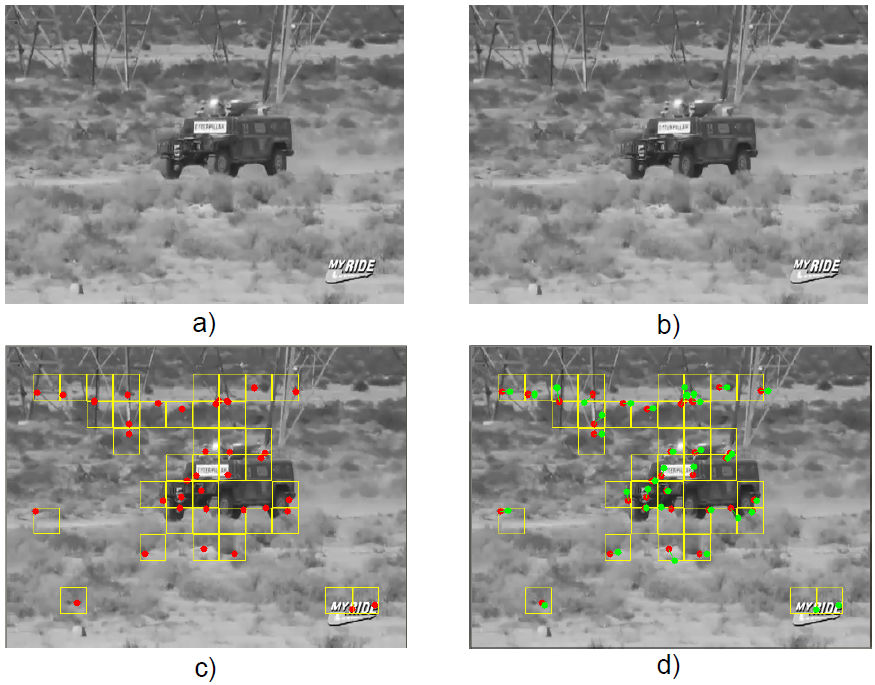
\includegraphics[scale=0.65]{img/3/of_example.png}
		\caption{Przykładowe wyznaczanie wektora przesunięcia -- źródło \cite{kryjak_14_vibe}}
		\label{fig:vibe_of_example}
	\end{figure}

\subsection{Detekcja narożników - metoda Harrisa-Stephensa}
\label{subsec:vibe_harris}

Algorytm detekcji narożników został opisany w publikacji \cite{harris_88}. Z punktu widzenia obliczeń opiera się on głównie na operacjach konwolucji. W pierwszej kolejności, należy określić tzw. macierz Harrisa, jej definicję przedstawia równanie (\ref{equ:vibe_harris_matrix}).

    \begin{equation}
        H = \begin{bmatrix}
               I_x^2 \otimes G    & I_x I_y \otimes G  \\
               I_x I_y \otimes G  & I_y^2 \otimes G    \\
     \end{bmatrix}
        \label{equ:vibe_harris_matrix}
    \end{equation}
Gdzie:
\begin{eqwhere}[2cm]
	\item[$I_x,\, I_y$] pierwsza pochodna obrazu wejściowego (pozioma i pionowa)
	\item[$\otimes G$] operacja konwolucji, wygładzenie obraz z wykorzystaniem filtru Gaussa
\end{eqwhere}

Pochodne pierwszego rzędu obrazu wejściowego są obliczane z wykorzystaniem filtru Prewitta, maska pozioma $P_x$ i pionowa $P_y$ zostały przedstawione równaniem (\ref{equ:vibe_prewitt}). Z kolei przykładowa maska filtru Gaussa (dla $\sigma = 3$) została opisana równaniem (\ref{equ:vibe_gauss}).

    \begin{equation}
        P_x = \begin{bmatrix}
			    -1 & 0 & +1 \\
			    -1 & 0 & +1 \\
			    -1 & 0 & +1 \\
		    \end{bmatrix}
		,\quad 
		P_y= \begin{bmatrix}
			    +1 & +1 & +1 \\
			    0 & 0 & 0 \\
			    -1 & -1 & -1 \\
		    \end{bmatrix}
        \label{equ:vibe_prewitt}
    \end{equation}

    \begin{equation}
       G(\sigma=3) = \begin{bmatrix}
			   0.1070 & 0.1131 & 0.1070 \\
			   0.1131 & 0.1196 & 0.1131 \\
			   0.1070 & 0.1131 & 0.1070 \\
		    \end{bmatrix}
        \label{equ:vibe_gauss}
    \end{equation}


Osteteczna odpowiedź detektora krawędzi wymaga obliczenia wyznacznika i śladu macierzy $H$. Finalna wartość może zostać zapisana równaniem (\ref{equ:vibe_harris_response}).
    \begin{equation}
        H_R = det(H)-k \cdot trace^2(H)
        \label{equ:vibe_harris_response}
    \end{equation}
Gdzie: $k$ - współczynnik skalowania (przyjmuje wartości \num{0.02} -- \num{0.2})


Po uwzględnieniu wzorów na wskaźnik i ślad macierzy o rozmiarze $2x2$, wzór (\ref{equ:vibe_harris_response}) można przekształcić do postaci (\ref{equ:vibe_harris_response_final}). Otrzymana wartość $H_R$ jest porównywana progowana. Jeżeli wartość progowa $H_{TH}$ zostanie przekroczona dany piksel uznawany jest za narożnik obiektu.  

    \begin{equation}
        H_R = I_x^2 \otimes G \cdot I_y^2 \otimes G - (I_x I_y \otimes G)^2  - k \cdot (I_x^2 \otimes G + I_y^2 \otimes G)^2
        \label{equ:vibe_harris_response_final}
    \end{equation}

\subsection{Uwagi}
\label{subsec:vibe_uwagi}

Algorytm \textit{ViBE} jest metodą zawierającą niezbyt złożony model tła oraz charakteryzującą się niedużą złożonością obliczeniową. Warto jeszcze raz podkreślić niewielką liczbę parametrów, ostateczna lista prezentują się następująco (w nawiasach podano wartości domyślne):\\
\-\hspace{1cm} $N$ -- liczba próbek w modelu tła ($20$)\\
\-\hspace{1cm} $\#_{min}$ -- minimalna liczba próbek wymagana w teście dopasowania ($2$)\\
\-\hspace{1cm} $R$ -- próg dopasowania próbki do modelu ($15$) \\
\-\hspace{1cm} $T$ -- prawdopodobieństwo wykonania aktualizacji ($\frac{1}{16}$)\\
\\
\noindent W przypadku rozszerzonej wersji algorytmu, należy uwzględnić jeszcze jeden dodatkowy parametr, mianowicie próg $H_{TH}$ (domyślnie $10$), wykorzystywany podczas detekcji krawędzi metodą Harrisa-Stephensa.
    

\section{Pixel-Based Adaptive Segmenter}
\label{sec:pbas_teoria}

Omawiany algorytm jest rozszerzeniem opisanej rozdziale \ref{subsec:vibe_opis} metody \textit{ViBE}. \textit{PBAS} (ang. \textit{Pixel Based Adaptive Segmenter}, podobnie jak opisana już wcześniej metoda, także posiada model, który składa się między innymi z próbek pochodzących z poprzednich ramek obrazu. Dodatkowo, próg dopasowania oraz prawdopodobieństwo dokonania aktualizacji są niezależne i na bieżąco uaktualniane dla każdego modelu. Opisywany algorytm może zostać zaimplementowany zarówno w wersji \textit{RGB} jak i w skali szarości.

Algorytm został zaprezentowany w artykule \cite{kryjak_14_pbas} i to właśnie na jego podstawie powstał niniejszy opis. Oprócz standardowej wersji metody \textit{PBAS} autorzy zaproponowali także dodatkowy mechanizm eliminacji tzw. ,,duchów'' (opis tego zjawiska został dokładnie opisany w rozdziale \ref{subsec:pbas_duchy}). Zaproponowane rozwiązanie opiera się na algorytmie etykietowania obiektów i następnie porównywania krawędzi na obrazie wejściowym i masce wyjściowej w odrębie każdego z nich.


\subsection{Opis algorytmu}
\label{subsec:pbas_opis}

Model tła jest nieco bardziej złożony niż ten przedstawiony w algorytmie \textit{ViBE}. Jego pierwsza część, podobnie jak w poprzedniej metodzie, składa się z $N$ zapamiętanych próbek. W celu uproszczenia dalszego zapisu matematycznego, zdefiniujmy ten zbiór jako $B(x_i)$, gdzie $x_i$ to aktualnie przetwarzany piksel obrazu, całość została opisana równaniem (\ref{equ:pbas_model_1}).

	\begin{equation}
		B(x_i)= \left\{ B_1(x_i), B_2(x_i), \dotsc, B_N(x_i) \right\}
	\label{equ:pbas_model_1}	
	\end{equation}

Test dopasowania, jest również bardzo podobny do tego, który występuje w metodzie \textit{ViBE}, jedyną różnicą jest niezależny dla każdego modelu próg przynależności do modelu $R(x_i)$, całość została przedstawiona równaniem (\ref{equ:pbas_test}).

	\begin{equation}
	    F(x_i) = 
		\begin{dcases}
    		1, & \text{gdy } \sum_{k=0}^{N} \{ d(I(x_i), B_k(x_i)) < R(x_i) \} < \#_{min} \\
    		0, & \text{w pozostałych przypadkach} 
		\end{dcases}
	\label{equ:pbas_test}	
	\end{equation}
\noindent Gdzie $d$ to funkcja odległości pomiędzy próbką z modelu tła, a aktualnym pikselem. 

W przypadku algorytmu w wersji \textit{RGB} każdy kanał przetwarzany jest osobno z wykorzystaniem niezależnego modelu tła. Finalna maska jest alternatywą logiczną wyników z poszczególnych kanałów, oznaczając poszczególne maski jako $F_R$, $F_G$, $F_B$ ostateczną klasyfikację możemy zapisać równaniem~(\ref{equ:pbas_final_mask}).

    \begin{equation}
        F_{RGB} = F_R \lor \lor F_G \lor F_B
    \label{equ:pbas_final_mask}
    \end{equation}


Ponieważ każdy kanał analizowany jest osobno, funkcję odległości pomiędzy próbkami można zapisać bardzo prosto równaniem (\ref{equ:pbas_dist}). Jest to po prostu moduł różnicy.
	\begin{equation}
		d(I(x_i),B_k(x_i)) = | I(x_i) - B_k(x_i) |
	\label{equ:pbas_dist}	
	\end{equation}

Kolejnym krokiem po przeprowadzeniu testu dopasowania i klasyfikacji piksela jest aktualizacja modelu tła. Zastosowano konserwatywne podejście, czyli aktualizowane są tylko piksele sklasyfikowane jako tło. Analogicznie jak w algorytmie \textit{ViBE} decyzja o aktualizacji podejmowana jest losowo. Prawdopodobieństwo jej wykonania wynosi $p = 1/T(x_i)$, gdzie parametr $T(x_i)$ jest dynamicznie aktualizowany i niezależny dla każdego piksela. Sama aktualizacja, polega na nadpisaniu, losowo wybranej próbki $B_k(x_i)$ z modelu aktualną wartością piksela $I(x_i)$. Dodatkowo, wybierany jest losowy piksela z otoczenia $3x3$ i losowo wybrana próbka z modelu mu odpowiadającego, jest nadpisywana wartością tego piksela.

Niezależnie od aktualizacji części modelu zawierającej zapamiętane próbki dokonywana jest zmiana parametrów $R(x_i)$ i $T(x_i)$. W tym celu konieczne jest zdefiniowanie kolejnego elementu modelu tła, który zawiera zbiór minimalnych odległości pomiędzy próbką z modelu a aktualną wartością piksela. Zbiór ten został opisany równaniem (\ref{equ:pbas_model_2}). 
 
	\begin{equation}
		D(x_i)= \left\{ D_1(x_i), D_2(x_i) \dotsc, D_N(x_i) \right\}
	\label{equ:pbas_model_2}	
	\end{equation}

Przedstawiony zbiór $D(x_i)$ aktualizowany jest razem ze zbiorem próbek. Nadpisywany jest jedynie element o indeksie $k$ dla którego dystans pomiędzy próbką i aktualnym pikselem jest najmniejsza, zostało to przedstawione równaniem (\ref{equ:pbas_d_min}).
	
	\begin{equation}
		d_{min}(x_i) = min_k d(I(x_i), B_k(x_i))
	\label{equ:pbas_d_min}	
	\end{equation}

Do aktualizacji progu dopasowania, czyli parametru $R(x_i)$ konieczne jest wyznaczenie tzw. miary dynamiki tła, czyli inaczej wartości średniej ze zbioru $D(x_i)$. Finalny wzór na nową wartość progu przedstawia równanie (\ref{equ:pbas_r_update}). Warto dodać, że przyjęto także dolne ograniczenie wartości parametru, wynoszące $R_{low} = 18$.
    
    \begin{equation}
	    R(x_i) = 
		\begin{dcases}
    		R(x_i)(1-R_{inc/dec}), & \text{jeżeli } R(x_i) > \bar{d}_{min}(x_i)R_{sc} \\
    		R(x_i)(1+R_{inc/dec}) & \text{w przeciwnym razie} 
		\end{dcases}
	\label{equ:pbas_r_update}	
	\end{equation}
Gdzie:
\begin{eqwhere}[2.2cm]
	\item[$R_{inc/dec}$] stały współczynnik aktualizacji (domyślnie $0.05$)
	\item[$\bar{d}_{min}(x_i)$] wartość średnia zbioru $D(x_i)$
	\item[$R_{sc}$] współczynnik skalowania (domyślnie $5$)
\end{eqwhere}

Ostatni etap to aktualizacja parametru opisującego prawdopodobieństwo dokonania aktualizacji, czyli $T(x_i)$. Nowa wartość zależy od wyniku klasyfikacji piksela i została opisana równaniem (\ref{equ:pbas_t_update}). Przyjęto założenie, że parametr ten posiada także ograniczenie dolne jak i górne wynoszące odpowiednio $T_{low}=2$ i $T_{up}=200$. 

    \begin{equation}
	    T(x_i) = 
		\begin{dcases}
    		T(x_i) + \frac{T_{inc}}{\bar{d}_{min}(x_i)}, & \text{jeżeli } F(x_i)=1 \\
    		T(x_i) - \frac{T_{dec}}{\bar{d}_{min}(x_i)} & \text{w przeciwnym razie} 
		\end{dcases}
	\label{equ:pbas_t_update}	
	\end{equation}


\subsection{Detekcja obiektów statycznych}
\label{subsec:pbas_duchy}

Autorzy publikacji \cite{kryjak_14_pbas} zaproponowali dodatkowy mechanizm eliminacji tzw. ,,duchów''. Przedstawiona metoda opiera się na porównaniu krawędzi na obrazie wejściowym i masce końcowej. Jeżeli krawędzie, na obu obrazach są identyczne, to znaczy, że obiekt rzeczywiście istnieje, natomiast w przeciwnym wypadku jest on duchem i zostaje usunięty z finalnej maski. 

Pierwszym krokiem, który należy wykonać w celu identyfikacji potencjalnych ,,duchów'' jest operacja odejmowania dwóch kolejnych ramek. W przestrzeni \textit{RGB} taka operacja jest opisana przez równanie (\ref{equ:pbas_cfd}).

    \begin{equation}
        dF(x_i) = \sum_{C \in \{R,G,B\}} | I(x_i)_{K}^C - I(x_i)_{K-1}^C |
    \label{equ:pbas_cfd}
    \end{equation}
    
\noindent Gdzie przez $I(x_i)_{K}^C$ rozumiemy wartość jednej ze składowych \textit{R,G,B} piksela o położeniu $x_i$ w $K$-tej ramce obrazu.

Kolejny etap to obliczenie tzw. współczynnika stabilność. Operację tą opisuje równanie (\ref{equ:pbas_stability}), jest ona wykonywana niezależnie dla każdego zidentyfikowanego obiektu na masce wyjściowej. Do tego celu konieczna jest także operacja indeksacji obiektów, ponieważ jest to zagadnienie dość złożone zostało opisane oddzielne w rozdziale \ref{subsec:pbas_indeksacja}. Sam współczynnik definiujemy jako stosunek liczby pikseli, których różnica opisana równaniem (\ref{equ:pbas_cfd}) przekracza ustalony próg $\theta$ do całkowitej powierzchni obiektu.

    \begin{equation}
        S_{O_k} = \frac{ \sum_{x_i \in O_k} dF(x_i) > \theta }{ \sum_{x_i \in O_k} F(x_i) }
    \label{equ:pbas_stability}
    \end{equation}
Gdzie:
\begin{eqwhere}[2cm]
	\item[$O_k$] $k$-ty obiekt na masce wyjściowej, wyznaczony algorytmem indeksacji
	\item[$F(x_i)$] maska wyjściowa ze standardowego algorytmu \textit{PBAS}
\end{eqwhere}

\noindent Obiekt jest uznawany za statyczny (czyli potencjalnego ducha), jeżeli wartość współczynnika $S_{O_k}$ przekracza ustalony próg $S_{TH}$ (domyślnie równy $0.1$). Takie działanie ma na celu eliminację błędnej klasyfikacji wynikającej z szumów i zakłóceń obrazu.


W celu weryfikacji, czy dany obiekt istniej zarówno na obrazie wejściowym jak i masce wyjściowej, użyty został mechanizm porównywania krawędzi. Sama detekcja krawędzi została zrealizowana z wykorzystaniem filtru Sobela. Przykładowe maski dla osi $X$ i $Y$ przedstawiono w równaniu (\ref{equ:pbas_sobel}). Operacja konwolucji z maską sobela realizowana jest osobno dla każdego kanału \textit{RGB}, następie obrazy wynikowe dla obu osi są sumowane i binaryzowanne ze stałym progiem $T_S$. Maska finalna stanowi alternatywę logiczną wyników z wszystkich kanałów.

    \begin{equation}
        S_x = \begin{bmatrix}
			    -1 & 0 & +1 \\
			    -2 & 0 & +2 \\
			    -1 & 0 & +1 \\
		    \end{bmatrix}
		,\quad 
		S_y = \begin{bmatrix}
			    +1 & +2 & +1 \\
			    0 & 0 & 0 \\
			    -1 & -2 & -1 \\
		    \end{bmatrix} 
    \label{equ:pbas_sobel}
    \end{equation}

Po wyznaczeniu krawędzi obrazu należy dla każdego obiektu obliczyć tzw. współczynnik podobieństwa krawędzi $EC_{O_k}$, został on przedstawiony za pomocą równania (\ref{equ:pbas_edge_coef}).  Jeżeli otrzymana wartość przekracza próg $0.5$ oznacza to, że obiekt istnieje, czyli występuje zarówno na obrazie wejściowym jak i masce wyjściowej. 

    \begin{equation}
        EC_{O_k} = \frac{ \sum_{x_i \in O_k} F_E(x_i) == 1 \land I_E(x_i) == 1 }{ \sum_{x_i \in O_k} F_E(x_i) == 1 }
    \label{equ:pbas_edge_coef}
    \end{equation}
Gdzie:
\begin{eqwhere}[2.2cm]
	\item[$F_E$] krawędzie na masce wyjściowej
	\item[$I_E$] maska zawierająca krawędzie na obrazie wejściowym
	\item[$O_k$] $k$-ty obiekt zidentyfikowany na masce wyjściowej
\end{eqwhere}


Schemat blokowy rozszerzonej wersji metody \textit{PBAS} został przedstawiony na rysunku \ref{fig:pbas_diagram}. Oprócz modułu obliczającego maskę pierwszoplanową z użyciem standardowego algorytmu \textit{PBAS} zawiera on dodatkowe bloki odpowiedzialne za wszystkie operacje opisane w niniejszym rozdziale. Moduł \textit{EDGE} służy do wyznaczania krawędzi na aktualnym obrazie wejściowym (oznaczonym jako $I_N$). Blok \textit{CFD} (ang. \textit{consecutive frame differencing}) oblicza różnicę dwóch ramek kolejnych ramek ($I_N$ i $I_{N-1}$) opisaną równaniem (\ref{equ:pbas_cfd}). Najbardziej złożonym elementem jest moduł \textit{CCA} (ang. \textit{Connected Component Analysis}). Jest w nim wykonywana indeksacja obiektów (opisana szczegółowo w rozdziale \ref{subsec:pbas_indeksacja}), wartością końcową tej operacji są parametry kwadratowego bloku otaczającego zidentyfikowany obiekt (ang. \textit{bounding box}). Oprócz tego są wyznaczane wartości $S_{O_k}$ i $EC_{O_k}$ -- równania (\ref{equ:pbas_stability}) i (\ref{equ:pbas_edge_coef}) oraz finalna maska wyjściowa. Obliczone współczynniki stabilności i podobieństwa krawędzi są przekazywane jako sprzężenie zwrotne do standardowego algorytmu \textit{PBAS}.

 
	\begin{figure}[h]
		\centering
		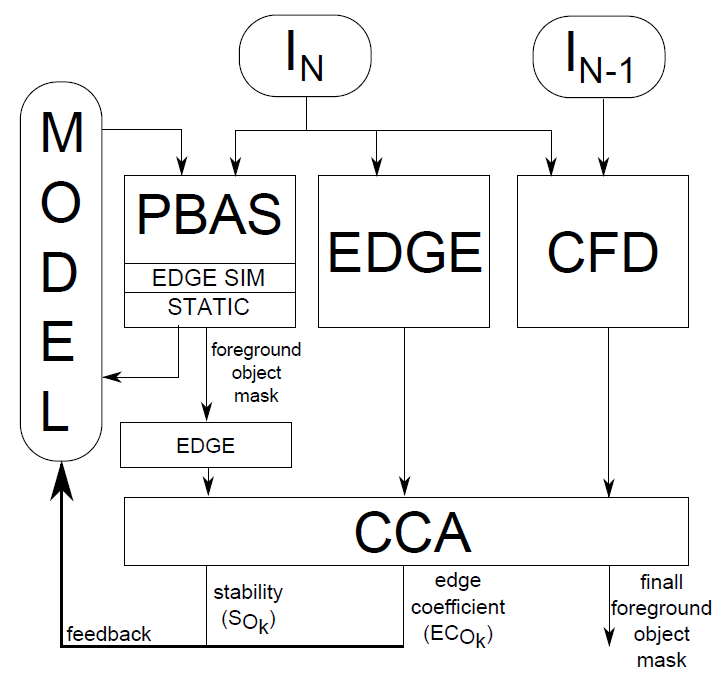
\includegraphics[scale=0.6]{img/3/pbas_diagram.png}
		\caption{Schemat blokowy rozszerzonej metody \textit{PBAS} -- źródło \cite{kryjak_14_pbas}}
		\label{fig:pbas_diagram}
	\end{figure}


Ostatnim krokiem jest obsługa sprzężenia zwrotnego, w tym celu do modelu tła zostały dodane dwa kolejne elementy. Pierwszym z nich jest licznik $S(x_i)_{cnt}$ określający przez ile ramek dany piksel był rozpoznawany jako obiekt statyczny. Sposób jego aktualizacji został opisany równaniem (\ref{equ:pbas_s_cnt}). 
    \begin{equation}
	    S(x_i)_{cnt} = 
		\begin{dcases}
    		S(x_i)_{cnt} + 1 & \text{jeżeli } S_{O_k} \geq  S_{TH}	 \\
            0                & \text{jeżeli } S_{O_k} <  S_{TH}	     \\		
    		S(x_i)_{cnt} - 1 & \text{w pozostałych przypadkach} 
		\end{dcases}
	\label{equ:pbas_s_cnt}	
	\end{equation}

\noindent Operacja ta jest przeprowadzana dla każdego piksela wewnątrz prostokąta otaczającego dany obiekt. Licznik jest inkrementowany dla obiektów zaklasyfikowanych jako statyczne, dla poruszających się zostaje wyzerowany, natomiast dla elementów tła jest dekrementowany.

Drugim dodatkowym elementem modelu jest średnia krocząca współczynnika podobieństwa krawędzi $EC(x_i)_{mean}$, jej wartość jest aktualizowana zgodnie z równaniem (\ref{equ:pbas_ec_mean}).

    \begin{equation}
	    EC(x_i)_{mean} = 
		\begin{dcases}
    		0.5EC(x_i) + 0.5EC(x_i)_{mean} & \text{jeżeli } S_{O_k} \geq  S_{TH} \land S(x_i)_{cnt} > S_{{cnt}_{TH}}	 \\
            1                & \text{w przeciwnym razie}		
		\end{dcases}
	\label{equ:pbas_ec_mean}	
	\end{equation}
\noindent Gdzie poprzez $S_{{cnt}_{TH}}$ oznaczamy minimalną liczbę ramek przez którą obiekt musi pozostać statyczny.
\\
\noindent Opisane parametry są wykorzystywane w procesie aktualizacji modelu, niezależnie od decyzji podjętej według standardowej procedury, model zostaje zaktualizowany jeżeli spełniony jest warunek logiczny opisany równaniem (\ref{equ:pbas_plus_update}).
    \begin{equation}
	    S_{O_k} \geq S_{TH} \land S(x_i)_{cnt} > S_{cnt_{TH}} \land EC(x_i)_{mean} < 0.5
	\label{equ:pbas_plus_update}	
	\end{equation}


\subsection{Indeksacja obiektów}
\label{subsec:pbas_indeksacja}

Opisany w rozdziale \ref{subsec:pbas_duchy} mechanizm detekcji tzw. ,,duchów'' wymaga rozróżnienia poszczególnych obiektów na wynikowej masce binarnej. W celu osiągnięcia takiego rezultatu, konieczne jest zastosowanie algorytmu indeksacji. Istnieje kilka podejść do realizacji tego zagadnienia, w niniejszej pracy zdecydowano się zastosować metodę jednoprzebiegową. Ze względu na jej stosunkowo prostą implementację w układach \textit{FPGA}. Problem implementacji sprzętowej został szerzej rozwinięty w rozdziale \ref{sec:fpga_pbas_plus}. 

Działanie algorytmu polega na nadawaniu poszczególnym pikselom etykiet reprezentujących kolejne obiekty, piksele z taką samą etykietą reprezentują ten sam obiekt. Oczekiwanym efektem końcowym, wymaganym w omawianym algorytmie jest pole, oraz parametry prostokąta, otaczającego każdy obiekt w danej ramce obrazu. Otaczający prostokąt jest reprezentowany przez cztery liczby $[x_1,y_1,x_2,y_2]$, gdzie współrzędne z indeksem 1 oznaczają lewy górny róg prostokąta, natomiast te z indeksem 2 prawy dolny róg. 

Pierwszym krokiem w procesie indeksacji jest wygenerowanie sąsiedztwa na podstawie którego aktualnie analizowany piksel będzie klasyfikowany. Jako sąsiedztwo, rozumiemy najbliższe otaczające piksele, ze względu na potokowe przetwarzanie obrazu wystarczy rozpatrzyć trzy piksele, znajdujące się w wyższym rzędzie oraz sąsiada po lewej stronie w rzędzie aktualnie analizowanym. Po wyznaczeniu sąsiedztwa, można przystąpić do klasyfikacji piksela. Jeżeli piksel ma wartość $1$ (jest elementem pierwszego planu) należy mu przypisać etykietę.  

Podczas operacji przypisania etykiety kolejnemu pikselowi mogą wystąpić trzy przypadki. Najprostszy z nich jest wtedy, gdy żaden z sąsiadujących pikseli nie ma przypisanej żadnej etykiety. W takiej sytuacji aktualny piksel traktowany jest jako fragment nowego obiektu i dostaje nową etykietę. Drugi przypadek to taki w którym, co najmniej jeden piksel posiada już przypisaną etykietą. Jeżeli pośród sąsiednich pikseli pojawia się tylko jedna etykieta oznacza to, że aktualny piksel także jest fragmentem obiektu oznaczonego właśnie tą etykietą, więc zostaje mu ona przypisana.
Ostatnim przypadkiem jest tzw. konflikt, występuje on wtedy, gdy pośród sąsiednich pikseli występują różne etykiety. Taka sytuacja może się przytrafić na przykład w sytuacji gdy analizowany jest obiekt w kształcie litery V. Warto zauważyć, że ze względu ma potokowe przetwarzanie obrazu w obszarze tego samego sąsiedztwa mogą istnieć tyko dwie różne etykiety. W przypadku wystąpienia kolizji oba obiekty łączone są w jeden.

Obszar oraz blok otaczający każdy obiekt, jest aktualizowany na bieżąco wraz z kolejnymi przetwarzanymi pikselami. W przypadku nowego obiektu, pole inicjializowane jest oczywiście wartością 1~natomiast współrzędne wierzchołków bloku otaczającego przyjmują współrzędne piksela. Dalsza aktualizacja pola obiektu wymaga jedynie inkrementacji wartości wraz z kolejnymi pikselami przypisanymi do danego obiektu. Blok otaczający jest natomiast aktualizowany na podstawie współrzędnych $x$ i $y$ aktualnego piksela, zgodnie z równaniem (\ref{equ:labeling_bbox_update}). 

    \begin{equation}
        (x_{1}, y_{1}, x_{2}, y_{2})= (min(x_{1}, x), min(y_{1}, y), max(x_{1}, x), max(y_{1}), y)
    \label{equ:labeling_bbox_update}
    \end{equation}

\noindent
W przypadku wystąpienia konfliktu, pola obu obiektów zostają zsumowane. Lewy górny róg zostaje ustawiony jako minimum spośród dwóch łączonych obiektów, natomiast prawy dolny jako maksimum.

%Do zaprezentowania pełnego zapisu matematycznego przyjęto następujące oznaczenia, niech $I$ oznacza obraz binarny z którego chcemy wyodrębnić poszczególne obiekty, zbiór $F$ zawiera wszystkie piksele białe (pierwszoplanowe), natomiast zbiór $B$ czarne (reprezentujące tło). Obiektem nazywamy z kolei zbiór $C$, będący podzbiorem $F$, taki że wszystkie piksele są połączone. Dwa piksele $P$ i $Q$ są połączone, jeżeli istnieje ścieżka utworzona z pikseli $(p_0, p_1, \dotsc , p_n)$, taka że $p_0=P$, $p_n=Q$ i każdy kolejny piksel jest sąsiadem poprzedniego. W tym przypadku przez sąsiedztwo rozumiane jest $8$ pikseli otaczających.%

\subsection{Uwagi}
\label{subsec:pbas_uwagi}

Przedstawiony algorytm jest rozszerzoną wersją omówionej w rozdziale \ref{sec:vibe_teoria} metody \textit{ViBE}. W tym przypadku wykorzystywany jest bardziej rozbudowany model tła, a sam algorytm charakteryzuje się większą złożonością obliczeniową. W stosunku do wcześniej omawianej metody, zwiększyła się także lista parametrów, kompletna lista została zamieszczona poniżej (w nawiasach umieszczono wartości domyślne):\\
\-\hspace{1cm} $N$ -- liczba próbek w modelu tła ($19$)\\
\-\hspace{1cm} $\#_{min}$ -- minimalna liczba próbek wymagana w teście dopasowania ($2$)\\
\-\hspace{1cm} $R_{init}$ -- początkowa wartość progu dopasowania próbki do modelu ($30$) \\
\-\hspace{1cm} $T_{init}$ -- początkowe prawdopodobieństwo wykonania aktualizacji ($\frac{1}{16}$)\\
\-\hspace{1cm} $R_{low}$ -- dolne ograniczenie progu dopasowania próbki do modelu ($18$) \\
\-\hspace{1cm} $T_{low}, \, T_{up} $ -- dolne i górne ograniczenie progu dopasowania próbki do modelu ($2$ i $200$) \\
\-\hspace{1cm} $R_{inc/dec}$ -- współczynnik wykorzystywany przy aktualizacji parametru $R$ (\num{0.05}) \\
\-\hspace{1cm} $R_{SC}$ -- współczynnik skalowania wykorzystywany przy aktualizacji parametru $R$ ($5$)\\
\\
\noindent W rozszerzonej wersji, zawierającej mechanizm detekcji duchów, należy uwzględnić jeszcze następujące parametry:\\
\-\hspace{1cm} $\theta$ -- próg wykorzystywany w (\ref{equ:pbas_stability}), określający ruchome obiekty ($50$)\\
\-\hspace{1cm} $S_{TH}$ -- wartość progowa współczynnika stabilności (\num{0.01})\\
\-\hspace{1cm} $S_{cnt_{TH}}$ -- minimalna liczba ramek przez która obiekt musi pozostać statyczny ($5$) \\
\-\hspace{1cm} $T_{S}$ -- próg binaryzacji wykorzystywany w detekcji krawędzi metodą Sobela ($50$)\\

\section{Gaussian Mixture Models}
\label{sec:gmm_teoria}

Metoda \textit{GMM} (ang. \textit{Gaussian Mixture Models}) jest algorytmem wykorzystującym statystyczny model tła. W przeciwieństwie do algorytmów opisywanych w poprzednich rozdziałach, tutaj model tła nie składa się z zapamiętanych próbek. Podobnie jak inne metody, ta także może przetwarzać obraz w różnych przestrzeniach barw. 

Jako, że jest to algorytm opublikowana po raz pierwszy w 1999 roku \cite{Stauffer_Grimson_99}, to od tamtej pory doczekała się wielu różnych odmian i udoskonaleń. Ponieważ tematem niniejszej pracy jest analiza i unifikacja algorytmów opracowanych w Laboratorium Biocybernetyki AGH w tym rozdziale zostanie zamieszczony opis powstały w oparciu o prace inżynierskie \cite{janus_15, piszczek_15}. W wyżej wymienionych publikacjach zamieszczono wyczerpujący opis metody, zarówno od strony teoretycznej jak i implementacyjnej, niniejsza praca zawiera jedynie podstawowe założenia i główne kroki algorytmu.


\subsection{Opis Algorytmu}
\label{subsec:gmm_opis}


Opisywany algorytm opiera się na modelu tła składającym się z $K$ rozkładów Gaussa, są one podzielone na dwa rodzaje, część z nich reprezentuje tło, reszta obiekty pierwszoplanowe. Model skonstruowany jest tak, że dla każdego piksela zdefiniowany jest osobny zestaw rozkładów Gaussa, który następnie jest niezależnie aktualizowany. Niewątpliwą zaletą w kontekście implementacji w układzie \textit{FPGA} jest brak jakichkolwiek operacji wykorzystujących otoczenie piksela, pozwala to zaoszczędzić dużą część zasobów. Szczegóły implementacji sprzętowej przedstawiono w rozdziale \ref{sec:fpga_gmm}.

Każdy rozkład Gaussa składa sie z trzech elementów: wagi ($\omega$), wariancji ($\sigma$) i wartości średniej ($\mu$). W przypadku przetwarzania obrazu w przestrzeni \textit{RGB}, w celu uproszczenie obliczeń, zakłada się, że waga i wariancja jest identyczna dla wszystkich trzech kanałów. Opierając się na publikacjach \cite{Stauffer_Grimson_99, piszczek_15}, liczbę rozkładów (parametr $K$) najlepiej przyjąć z zakresu $3$ -- $5$.  


Pierwszym krokiem jest posortowanie rozkładów Gaussa według współczynnika $r_i = \frac{\omega_i}{\sigma_i}$ w kolejności rosnącej (przez $i$ rozumiemy numer rozkładu, natomiast $\omega_{i,t}$ oznacza wagę i-tego rozkładu w czasie t). Ze względu na przyjęte uproszczenie, że wariancja jest identyczna dla wszystkich kanałów RGB, macierz kowariancji i-tego rozkładu w chwili t może zostać zapisana równaniem (\ref{equ:gmm_cov}).

    \begin{equation}
        \Sigma_{i,t} = \sigma_{i,t}^2 I
    \label{equ:gmm_cov}
    \end{equation}

Zastosowanie sortowania według współczynnika $r_i$ powoduje umieszczenie na początku listy tych rozkładów, które najprawdopodobniej reprezentują tło (czyli tych o o najwyższej wadze oraz najniższej wariancji). Przyjęto, że pierwsze $B$ rozkładów z listy uznaje się za rozkładu reprezentujące tło, kolejne to już obiekty pierwszoplanowe. Jak łatwo zauważyć, rozkłady przedstawiające tło, mają zdecydowanie wyższą wagę oraz niewielką wariancję. Równanie (\ref{equ:gmm_b}) określa wartość $B$, jest to liczba rozkładów, dla których suma wag przekracza próg $T$.


    \begin{equation}
        B = arg\,min_b \left(\sum_{i=1}^{b} \omega_{i,t} > T\right)
    \label{equ:gmm_b}
    \end{equation}

Kolejnym etap to test dopasowania nowego piksela do modelu. Przeprowadzany jest on dla każdego rozkładu Gaussa z posortowanej listy i~przerywany w momencie uzyskania pozytywnego wyniku (piksel wejściowy pasuje do modelu). Jeżeli przyjmiemy, że nowy piksel pojawia się w chwili $t+1$ to test dopasowania przeprowadzany jest z modelem z~chwili $t$. Pozytywny wynik testu określa zależność (\ref{equ:gmm_mahalanobis}).

    \begin{equation}
        \sqrt{ \left( \left( X_{t+1} - \mu_{i,t} \right)^T \cdot \Sigma_{i,t}^{-1} \cdot \left( X_{t+1} - \mu_{i,t} \right) \right)} < k \sigma_{i,t}
    \label{equ:gmm_mahalanobis}
    \end{equation}

\noindent Gdzie próg $k$ domyślnie przyjmuje wartość \num{2.5}


Na tym etapie algorytmu, należy rozważyć dwa przypadki. Jeżeli piksel wejściowy został dopasowany do jednego z $K$ rozkładów Gaussa, to zostaje on klasyfikowany na podstawie wcześniejszej przynależności danego rozkładu, zgodnie z (\ref{equ:gmm_b}). Podczas aktualizacji modelu, zostanie wykorzystany parametr $\alpha$ określający stałą uczenia. Parametry rozkładu Gaussa, który przeszedł test dopasowania określony równaniem (\ref{equ:gmm_mahalanobis}), zostaje zaktualizowany według zależności (\ref{equ:gmm_w_update}), (\ref{equ:gmm_u_update}) i (\ref{equ:gmm_sigma_update}).

    \begin{equation}
        \omega_{i, t+1} = (1-\alpha)\omega_{i,t} + \alpha
    \label{equ:gmm_w_update}
    \end{equation}

    \begin{equation}
        \mu_{i, t+1} = (1-\rho)\mu_{i,t} + \rho X_{t+1}
    \label{equ:gmm_u_update}
    \end{equation}

    \begin{equation}
        \sigma_{i, t+1}^2 = (1-\rho)\sigma_{i,t}^2 + \rho (X_{t+1} - \mu{i,t+1})(X_{t+1} - \mu{i,t+1})^T
    \label{equ:gmm_sigma_update}
    \end{equation}

\noindent Do przedstawienia funkcji $\rho$ konieczna jest także definicja funkcji gęstości prawdopodobieństwa, która jest opisana równaniem (\ref{equ:gmm_density}). Z kolei samą funkcję $\rho$ przedstawia równanie (\ref{equ:gmm_rho}).

    \begin{equation}
        \eta (X_t, \mu, \Sigma) = \frac{1}{(2\pi)^{n/2} |\Sigma|^{1/2}} e^{-\frac{1}{2} (X_t - \mu)\Sigma^{-1} (X_t - \mu)} 
    \label{equ:gmm_density}
    \end{equation}
gdzie:
\begin{eqwhere}[2cm]
	\item[$X_t$] wartość piksela w chwili t
	\item[$\mu$] wektor wartości średnich rozkładu Gaussa
	\item[$\Sigma$] macierz kowariancji -- wzór (\ref{equ:gmm_cov})\\
\end{eqwhere}


    \begin{equation}
        \rho = \alpha \eta(X_{t+1}, \mu_{i}, \Sigma_{i})
    \label{equ:gmm_rho}
    \end{equation}

Reszta rozkładów, która nie przeszła testu dopasowania, zostaje zaktualizowana według równania (\ref{equ:gmm_unmatched_update}), nadpisywana jest tylko waga, wartość średnia i wariancja pozostają niezmienione.

    \begin{equation}
        \omega_{j,t+1} = (1-\alpha)\omega_{j,t}
    \label{equ:gmm_unmatched_update}
    \end{equation}

Drugim przypadek to piksel niepasujący do żadnego rozkładu. W takiej sytuacji jest on automatycznie klasyfikowany jest jako element pierwszoplanowy. Aktualizacja modelu w tym przypadku polega na zastąpieniu rozkładu o najniższej wadze nowym. Sama waga pozostaje niezmieniona, natomiast aktualna wartość piksela zapisywana jest jako wartość średnia. Przypisywana jest także duża wariancja inicjalizująca, która jest określona globalnie jako parametr całego algorytmu. \\

Warto jeszcze raz nadmienić, że powyższe operacje wykonywane są cyklicznie dla każdego piksela z wykorzystaniem niezależnego modelu tła. Lista wszystkich parametrów algorytmu \textit{GMM} przedstawia się następująco: \\
\-\hspace{1cm} $K$ -- liczba rozkładów Gaussa\\
\-\hspace{1cm} $T$ -- próg z przedziału $0$--$1$ pozwalający rozgraniczyć rozkłady tła i pierwszoplanowe\\
\-\hspace{1cm} $k$ -- współczynnik używany w teście dopasowania (\ref{equ:gmm_mahalanobis})\\
\-\hspace{1cm} $\alpha$ -- współczynnik uczenia z przedziału $0$--$1$\\
\-\hspace{1cm} $\sigma_{init}$ -- wariancja, którą inicjalizowany jest nowy gaussian\\ 


\subsection{Uwagi}
\label{subsec:gmm_uwagi}

Algorytm opisany w niniejszym rozdziale, przedstawia nieco odmienne podejście do segmentacji obiektów pierwszoplanowych w stosunku do metod opisanych wcześniej. Jak już zostało wspomniane w rozdziale \ref{cha:przeglad_metod} algorytm \textit{GMM} jest bardzo rozległym zagadnieniem, będącym przedmiotem badań wielu publikacji \cite{Stauffer_Grimson_99, Genovese_Napoli_13, piszczek_15, wang_14}. Ze względu na skomplikowane operacje matematyczne z punktu widzenia układów \textit{FPGA}, sama implementacja również jest dość złożonym problemem.

Jak słusznie zauważyli autorzy przytoczonych publikacji, algorytm \textit{GMM} zapewnia zadowalające rezultaty, aczkolwiek jest bardzo podatny na różnego rodzaju zakłócenia, szumy i zmiany oświetlenia. Mimo to w większość przypadków, jest to metoda, mogąca z powodzeniem zostać wykorzystana jako samodzielny system segmentacji tła.  



\chapter{Implementacja sprzętowa wybranych algorytmów}
\label{cha:implementacja_sprzetowa}

\section{Modele programowe}
\label{sec:modele_programowe}

\section{Wykorzystany układ oraz interfejs wizyjny}
\label{sec:uklad_interfejs}

Do implementacji algorytmów wykorzystano środowisko \textit{Vivado}. Użyto najnowszej wersji, na moment tworzenia niniejszej pracy (czerwiec 2017), oznaczonej numerem \textit{2017.1}. Większość modułów zaimplementowano w języku \textit{Verilog}. W pojedynczych przypadkach wykorzystano również język \textit{VHDL}. Wszystkie metody uruchomiono i sprawdzono na płytce \textit{VC707} z układem \textit{Virtex-7 (\small{XC7VX485T--2FFG1761})}. Jest to jeden z najwydajniejszych układów firmy \textit{Xillinx}. Dodatkowo w celu podłączenia kamery i transmisji obrazu wykorzystano kartę \textit{Avnet DVI I/O FMC}. Przyjęto założenie, że zaimplementowane algorytmy mają pracować w rozdzielczość \textit{720x576} w 50 klatkach na sekundę. Opcjonalnie obsługiwana może być również rozdzielczość \textit{1280x720} i \textit{1920x1080}, również z prędkością \textit{50 fps} (ang. \textit{Frames Per Second} -- klatki na sekundę). 
%Oprócz implementacji sprzętowych, dla każdego algorytmu przygotowano także model programowy. Modele te zostały zaimplementowane w języku \textit{C++} z wykorzystaniem biblioteki \textit{OpenCV} \cite{opencv_17}. Całość przygotowano w środowisku programistycznym \textit{Microsoft Visual Studio 2015}.

W przypadku implementacji sprzętowej w układzie \textit{FPGA} został wykorzystany uniwersalny interfejs wizyjny. Jego układ, przedstawiający podstawowe sygnały wejściowe i wyjściowe, został pokazany na rys. \ref{fig:fpga_vision_if}. Oprócz sygnałów wejściowych/wyjściowych z kamery, konieczne jest także zapewnienie niezależnego obszar pamięci \textit{RAM} dla każdego piksela. Maksymalnie do wykorzystania są 1024 bity na piksel w przypadku obrazu o rozdzielczości \textit{720x576} oraz 256 bitów dla wyższych rozdzielczości (\textit{720}p i \textit{1080}p). Sygnały pochodzące z kamery zostały szerzej opisane w rozdziale \ref{subsec:fpga_kontekst}. Należy zwrócić uwagę, że przedstawiony tutaj interfejs, zawiera jedynie niezbędne sygnały do funkcjonowania systemu. W przypadku niektórych algorytmów został on rozszerzony o dodatkowe wejścia/wyjścia. 

		\begin{figure}[h!]
				\centering
				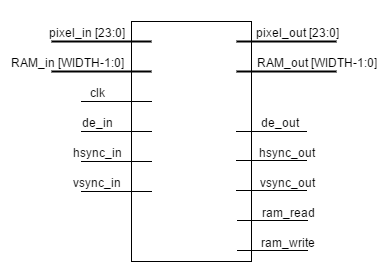
\includegraphics[scale=0.75]{img/4/vision_if.png}
				\caption{Główny interfejs wizyjny}
				\label{fig:fpga_vision_if}
		\end{figure}

\noindent \\Moduł przedstawiony na rys. \ref{fig:fpga_vision_if} posiada następujące sygnały wejściowe:\\
\-\hspace{1cm} \textit{pixel\_in} -- wartość piksela wejściowego w formacie RGB (24 bity)\\
\-\hspace{1cm} \textit{bg\_model\_in} -- odczytana pamięć RAM o długości \textit{WIDTH} (maksymalnie 1024 bity)\\
\-\hspace{1cm} \textit{clk} -- zegar piksela\\
\-\hspace{1cm} \textit{de\_in} -- flaga poprawności piksela wejściowego\\
\-\hspace{1cm} \textit{hs\_in} -- flaga synchronizacji poziomej\\
\-\hspace{1cm} \textit{vs\_in} -- flaga synchronizacji pionowej\\\\
%
Natomiast sygnałami wyjściowymi są:\\
\-\hspace{1cm} \textit{pixel\_out} -- wartość piksela wyjściowego w formacie RGB (24 bity)\\
\-\hspace{1cm} \textit{bg\_model\_out} -- blok o długości \textit{WIDTH} do zapisania w pamięci RAM (maksymalnie 1024 bity)\\
\-\hspace{1cm} \textit{de\_out} -- opóźniona flaga poprawności piksela wejściowego\\
\-\hspace{1cm} \textit{hs\_out} -- opóźniona flaga synchronizacji poziomej\\
\-\hspace{1cm} \textit{vs\_out} -- opóźniona flaga synchronizacji pionowej\\
\-\hspace{1cm} \textit{ram\_read} -- sygnał odczytu pamięci RAM\\
\-\hspace{1cm} \textit{ram\_write} -- sygnał zapisu do pamięci RAM\\

\section{Trudności występujące w potokowym systemie wizyjnym}
\label{sec:fpga_wprowadzenie}

\subsection{Kontekst poziomy i pionowy}
\label{subsec:fpga_kontekst}

Algorytmy wizyjne w układach FPGA, jak już zostało wspomniane, są realizowane w systemie potokowym. Oznacza to, że ramka obrazu przetwarzana jest piksel po pikselu. W związku z tym, w celu wykonania operacji kontekstowej koniecznej jest zastosowanie odpowiednich opóźnień. Dla kontekstu poziomego nie jest to duży problem i może zostać rozwiązany z wykorzystaniem zwykłych rejestrów. Natomiast w przypadku kontekstu pionowego konieczne jest zastosowanie opóźnienia o całą linie obrazu. Do tego celu, wykorzystuje się dostępną w układach FPGA pamięć blokową (\textit{BRAM}). Przykładowy system linii opóźniających, służących do wyznaczenia kontekstu o rozmiarze \textit{5x5} został przedstawiony na rysunku \ref{fig:fpga_delay_line}. Poprzez pojedynczy blok \textbf{D} rozumiemy opóźnienie o jeden takt zegara, z kolei stała \textit{H\_SIZE} definiuje ilość pikseli w jednej linii obrazu.

	\begin{figure}[h!]
	    \centering
		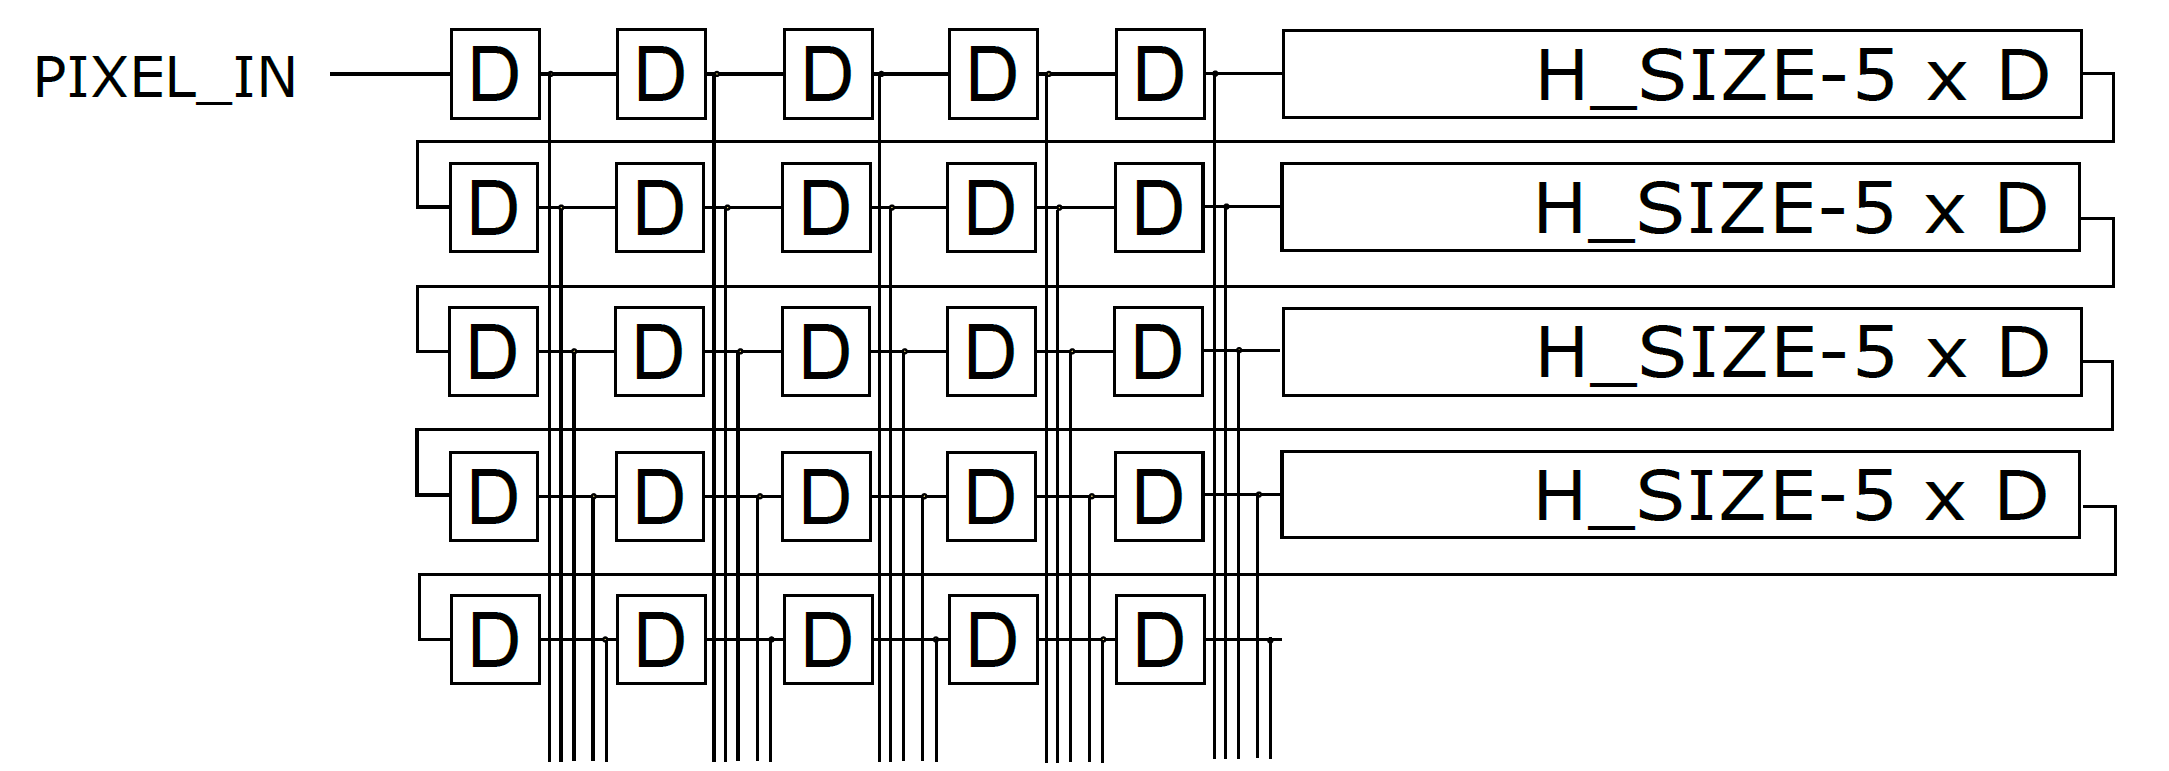
\includegraphics[scale=0.2]{img/4/context.png}
		\caption{Schemat długiej linii opóźniającej - źródło \cite{komorkiewicz_14}}
		\label{fig:fpga_delay_line}
	\end{figure}
	
Podczas ustalania parametru \textit{H\_SIZE} należy zwrócić uwagę na tzw. obszar synchronizacji. W rzeczywistość ilość pikseli przesyłanych w jednej ramce obrazu jest większa niż sugerowałaby rozdzielczość obrazu. Przykładowo, dla obrazu o rozdzielczości \textit{640x480} pikseli, rzeczywista liczba pikseli, po uwzględnieniu obszaru synchronizacji wynosi \textit{800x600}. Zostało to przedstawione na rysunku \ref{fig:fpga_sync_signals}. Wielkość obszaru synchronizacji zależy zarówno od rozdzielczości obrazu jak i liczby klatek na sekundę. Przy wyznaczaniu odpowiedniej długości, wymaganej linii opóźniającej, pomocna może okazać się baza danych \textit{Modeline Database} \cite{modeline_db_web}. W niniejszej pracy wykorzystano trzy rozdzielczości: \textit{720x576}, \textit{1280x720}, \textit{1920x1080} przy prędkości \textit{50 fps}. Całkowita długość linii poziomych, dla takich konfiguracji, wynosi odpowiednio: \textit{864}, \textit{1680}, \textit{2640}.

	\begin{figure}[h!]
        \centering
		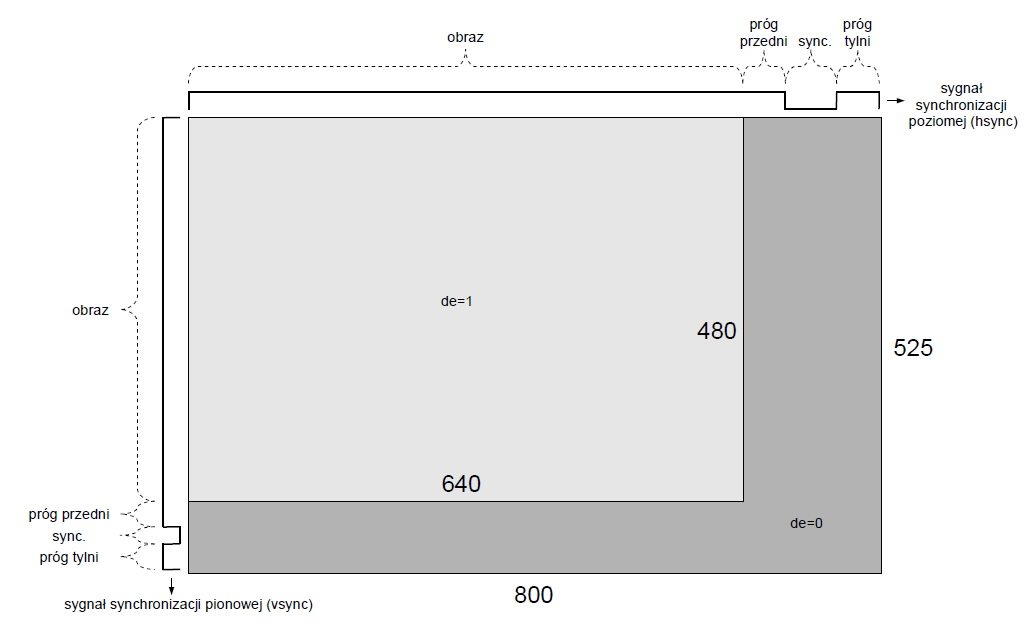
\includegraphics[scale=0.55]{img/4/sync_signals.png}
		\caption{Synchronizacja dla obrazu o rozdzielczości 640x480 -- źródło \cite{komorkiewicz_14}}
		\label{fig:fpga_sync_signals}
	\end{figure}


\subsection{Generowanie liczb losowych}
\label{subsec:fpga_generator}

Moduł odpowiedzialny za generację liczb pseudolosowych został opracowany na podstawie publikacji \cite{thomas_10}. Wykorzystano go także w wielu innych badań przeprowadzanych w Laboratorium Biocybernetyki AGH, między innymi \cite{kryjak_14_vibe, kryjak_14_pbas}. W przeciwieństwie do pozostałych modułów i algorytmów, generator został w całości zaimplementowany w języku \textit{VHDL}.

Zagadnienie liczb pseudolosowych w układach reprogramowalnych jest tematem bardzo rozległym i został dokładnie opisane w przytoczonym artykule. W niniejszym rozdziale zostanie przedstawiona jedynie skrótowa idea działania wykorzystanego generatora. Cała koncepcja opiera się na wykorzystaniu rejestrów przesuwnych (ang. \textit{shift register}) i modułów \textit{LUT} (ang. \textit{Look-Up Table}). Uproszczony schemat, tego typu generatora, zamieszczono na rysunku \ref{fig:fpga_rng}. Wartości wyjściowe są zapisywane w rejestrach przesuwnych o różnych długościach. Następnie różne kombinacje zapamiętanych bitów są podawane na wejścia bramek \textit{XOR}, które generują pseudolosowy sygnał wyjściowy.

	\begin{figure}[h!]
        \centering
		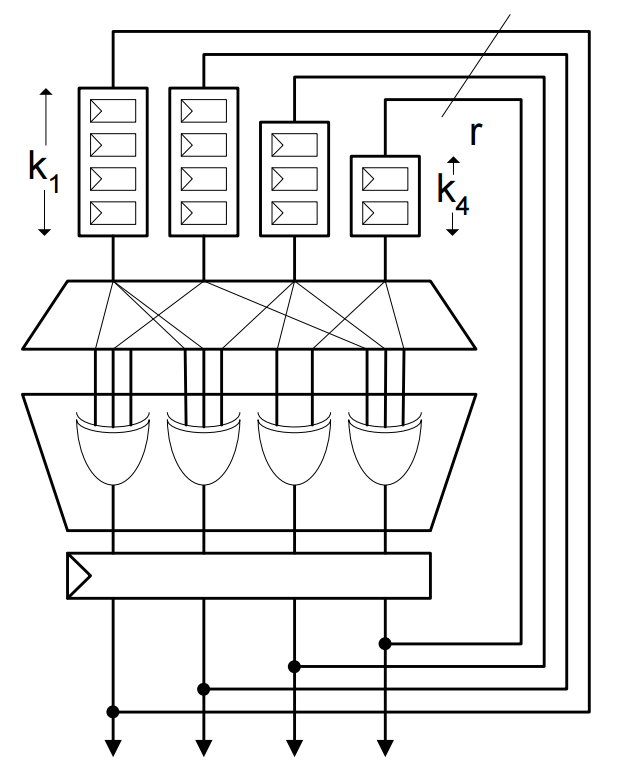
\includegraphics[scale=0.3]{img/4/rng_scheme.png}
		\caption{Schemat generatora liczb pseudolosowych -- źródło \cite{thomas_10}}
		\label{fig:fpga_rng}
	\end{figure}

Architekturę generatora można opisać za pomocą zestawu 4 parametrów ($n$, $r$, $t$, $k$), gdzie:\\
\-\hspace{1cm} \textit{n} -- liczba stanów generatora (okres możemy zapisać jako $2^n-1$)\\
\-\hspace{1cm} \textit{r} -- liczba bitów generowanych w każdym cyklu\\
\-\hspace{1cm} \textit{t} -- liczba wejść każdej bramki \textit{XOR}\\
\-\hspace{1cm} \textit{k} -- maksymalna długość rejestru przesuwnego\\

Wykorzystany w niniejszej pracy generator posiada następujące parametry: $n=3900$, $r=128$, $t=5$, $k=32$. Istnieje jeszcze jeden dodatkowy parametr $s$, który określa sposób połączeń wyjść rejestrów przesuwnych z bramkami \textit{XOR}. Dokładny algorytm, opisujący sposób doboru optymalnych połączeń, jest bardzo zaawansowanym zagadnieniem, wybiegającym poza tematykę niniejszej pracy. Szczegółowy opis i analiza tego podejścia została przedstawiona w przytoczonej publikacji.

\subsection{Kontroler pamięci RAM}
\label{subsec:fpga_ram_kontroler}

Kontroler pamięci \textit{RAM DDR3}, jest niezbędnym elementem, koniecznym do prawidłowego działa każdego rozbudowanego systemu wizyjnego. Zewnętrzna pamięć, jest bowiem niezbędna do przechowywania modelu tła dla poszczególnych pikseli. Przedstawiony kontroler, został opracowany w Laboratorium Biocybernetyki AGH w ramach publikacji \cite{kryjak_14_hd_fpga}. Podobnie jak w przypadku generatora liczb pseudolosowych, rozdział ten ma na celu jedynie przedstawienie uproszczonej koncepcji działania modułu. Dokładny opis i dyskusja zostały zawarte w przytoczonej publikacji. \textit{Xillinx} zapewnia dedykowany moduł \textit{MIG} (\textit{Memory Interface Generator}) do komunikacji z zewnętrzną pamięcią \textit{RAM}. Schemat kontrolera pamięci, wykorzystującego \textit{MIG} został przedstawiony na rysunku \ref{fig:ram_ctrl}. 

	\begin{figure}[h!]
		\centering
		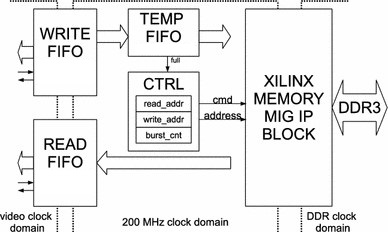
\includegraphics[scale=0.9]{img/4/ram_ctrl_scheme.jpg}
		\caption{Schemat kontrolera pamięci \textit{RAM} -- źródło \cite{kryjak_14_hd_fpga}}
		\label{fig:ram_ctrl}
	\end{figure}

Ze względu na fakt, że pamięć \textit{RAM} synchronizowana jest innym zegarem niż sygnał z kamery konieczne jest zastosowanie buforów w postaci dodatkowych kolejek \textit{FIFO}. Omawiany kontroler został zaimplementowany jako maszyna stanów. Podczas etapu inicjalizacji zapełniona zostaje w całości kolejka \textit{READ FIFO}. Następnie, w momencie gdy pojawi się na wejściu nowa ramka obrazu, modele tła z kolejki \textit{READ FIFO} zostają odczytywane i przekazywane do modułu realizującego algorytm segmentacji tła. Zaktualizowany model tła otrzymany na wyjściu, jest umieszczany w kolejce \textit{WRITE FIFO}. Kolejnym krokiem jest przeniesienie danych z kolejki \textit{WRITE FIFO} do dużo krótszej \textit{TEMP FIFO}. W~momencie, gdy kolejka ta jest zapełniona, uruchamiany jest tryb \textit{burst}, zapisujący wszystkie modele do pamięci \textit{RAM}. Po dokonaniu zapisu, dokładnie taka sama liczba modeli, zostaje odczytana z pamięci \textit{RAM} i ponownie umieszczona w kolejce \textit{READ FIFO}. Następnie kontroler przechodzi do stanu oczekiwania, aż do momentu ponownego zapełnienia się kolejki \textit{TEMP FIFO}.

\section{Implementacja algorytmu ViBE}
\label{sec:fpga_vibe}

Przygotowana implementacja sprzętowa, powstała na podstawie opisu teoretycznego metody, przedstawionego w rozdziale \ref{sec:vibe_teoria}, wykorzystano wersję operującą w przestrzeni \textit{CIELab}.  Wysokopoziomowy schemat implementacji, zawierający główny moduł realizujący algorytm, wejściowy i wyjściowy sygnał z kamery oraz połączenie z pamięcią RAM, został przedstawiony na rysunku \ref{fig:vibe_diagram}. Dla zachowania spójności, w dalszej części opisu, przyjęto oznaczenia parametrów algorytmu identyczne jak te zestawione w podsumowaniu rozdziału teoretycznego (podrozdział \ref{subsec:vibe_uwagi}).

	\begin{figure}[h!]
		\centering
		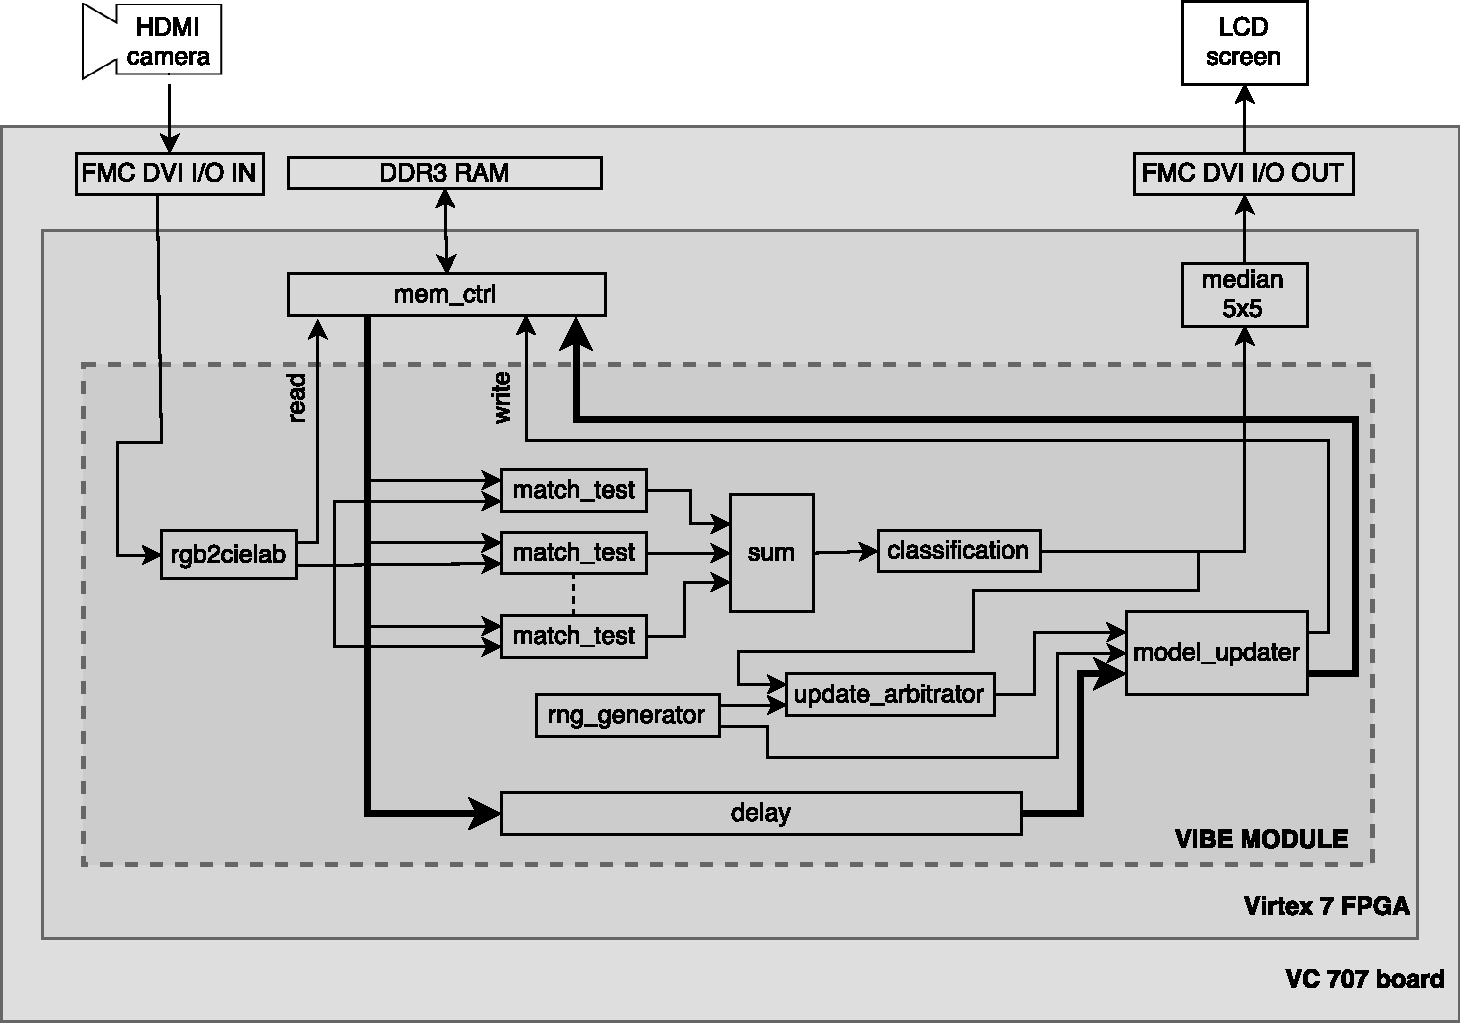
\includegraphics[scale=0.6]{img/4/vibe.pdf}
		\caption{Wysokopoziomowy schemat implementacji algorytmu \textit{ViBE}}
		\label{fig:vibe_diagram}
	\end{figure}

W podstawowej wersji algorytmu, wykorzystany został, standardowy interfejs wizyjny, przedstawiony na rysunku \ref{fig:fpga_vision_if}, bez żadnych dodatkowych sygnałów. Pierwszą operacją, jest oczywiście konwersja z przestrzeni \textit{RGB} do \textit{CIELab} (moduł \textit{rgb2cielab}). Operacja przekształcenia do macierzy \textit{XYZ}, opisana równaniem (\ref{equ:vibe_rgb_xyz}), jest prosta do zaimplementowania w logice programowej i została zrealizowana z wykorzystaniem mnożarek sprzętowych operujących na liczbach stałoprzecinkowych. Obliczanie wartości funkcji $f(t)$ zdefiniowanej równaniem (\ref{equ:vibe_f_t}) zostało zaimplementowane z użyciem operacji \textit{LUT} (ang. \textit{Look-Up Table}). Zastosowano trzy moduły, przechowujące stablicowane wartości funkcji $f(\frac{X}{X_n})$, $f(\frac{Y}{Y_n})$, $f(\frac{Z}{Z_n})$ wymagane do obliczenia składowych $a$ i $b$ danych równaniem (\ref{equ:vibe_xyz_cielab}) oraz jeden moduł zawierający wartości składowej $L$. Jak zostało już wspomniane w rozdziale \ref{subsec:vibe_cielab} składowe $a$ i $b$ mieszczą się w przedziale $-128$ do $127$. Natomiast składowa $L$ w zakresie $0$ -- $100$. W związku z tym rozmiar piksela to \textbf{23 bity} zamiast 24, jak miało to miejsce w przypadku przestrzeni \textit{RGB}.

Dla poszczególnych próbek modelu obliczany jest dystans do aktualnego piksela zgodnie z równaniem (\ref{equ:vibe_cielab_test}). Otrzymana wartość zostaje porównywana z progiem $R$. Operacje te wykonywane są równolegle dla każdej próbki z wykorzystaniem bloczków \textit{match\_test}. Następnie w module \textit{sum}, zliczane są próbki dla których test dopasowania przeszedł pozytywnie. Ostatnim etapem jest blok \textit{classification} dokonujący ostatecznej klasyfikacji piksela zgodnie z równaniem (\ref{equ:vibe_match_test}). Dodatkowo, w celu eliminacji szumów, na maskę wyjściową nakładany jest filtr medianowy o rozmiarze $5x5$.

W procesie aktualizacji modelu wykorzystywany jest, $128$ bitowy, losowy sygnał otrzymany z bloku \textit{rng\_generator}. Idea działania generatora liczb losowych została szerzej opisana w rozdziale \ref{subsec:fpga_generator}. Modułu \textit{update\_arbitrator} jest wykorzystywany do podejmowania decyzji odnośnie aktualizacji. Sama aktualizacja wykonywana jest natomiast w bloku \textit{model\_updater}. W tym celu, generowany jest kontekst o rozmiarze $3x3$, zawierający modele tła sąsiadujących pikseli. Na podstawie informacji, otrzymanych z modułu \textit{update\_arbitrator}, aktualizowany jest model piksela oraz losowo wybranego sąsiada. Następnie nowy model zostaje zapisany do pamięci \textit{RAM}. Warto zwrócić uwagę, że model jest odczytywany z pamięci po konwersji do przestrzeni \textit{CIELab}, aby wykorzystać go w procesie aktualizacji, konieczne jest zastosowanie linii opóźniającej o długości równej latencji procesu klasyfikacji piksela, operacja ta została zrealizowana przez moduł \textit{delay}.

Przedstawioną implementację udało się uruchomić w rozdzielczościach: \textit{576p}, \textit{720p}, \textit{1080p}. Na rysunku \ref{fig:vibe_demo} przedstawiono zdjęcie działającego systemu. W przypadku najniższej rozdzielczości przyjęto model składający się z $N=20$ próbek (rozmiar modelu wynosi w tym przypadku $20 \cdot 23=460$ bitów). Dla wyższych rozdzielczości, ze względu na ograniczenia pamięci \textit{RAM}, musiał on zostać ograniczony do $10$ (rozmiar modelu równy $10 \cdot 23=230$ bity). Pozostałym parametrom przypisano wartości domyślne, zostały one zapisane jako liczny całkowite. Wyjątkiem jest parametr $T$, opisujący prawdopodobieństwo wykonania aktualizacji, w tym przypadku została wykorzystana 16 bitowa liczba stałoprzecinkowa (ang. \textit{fixed float}) bez znaku o oznaczeniu \textit{8z8u}, czyli po 8 bitów przeznaczonych na część całkowitą i ułamkową.

	\begin{figure}[h!]
		\centering
		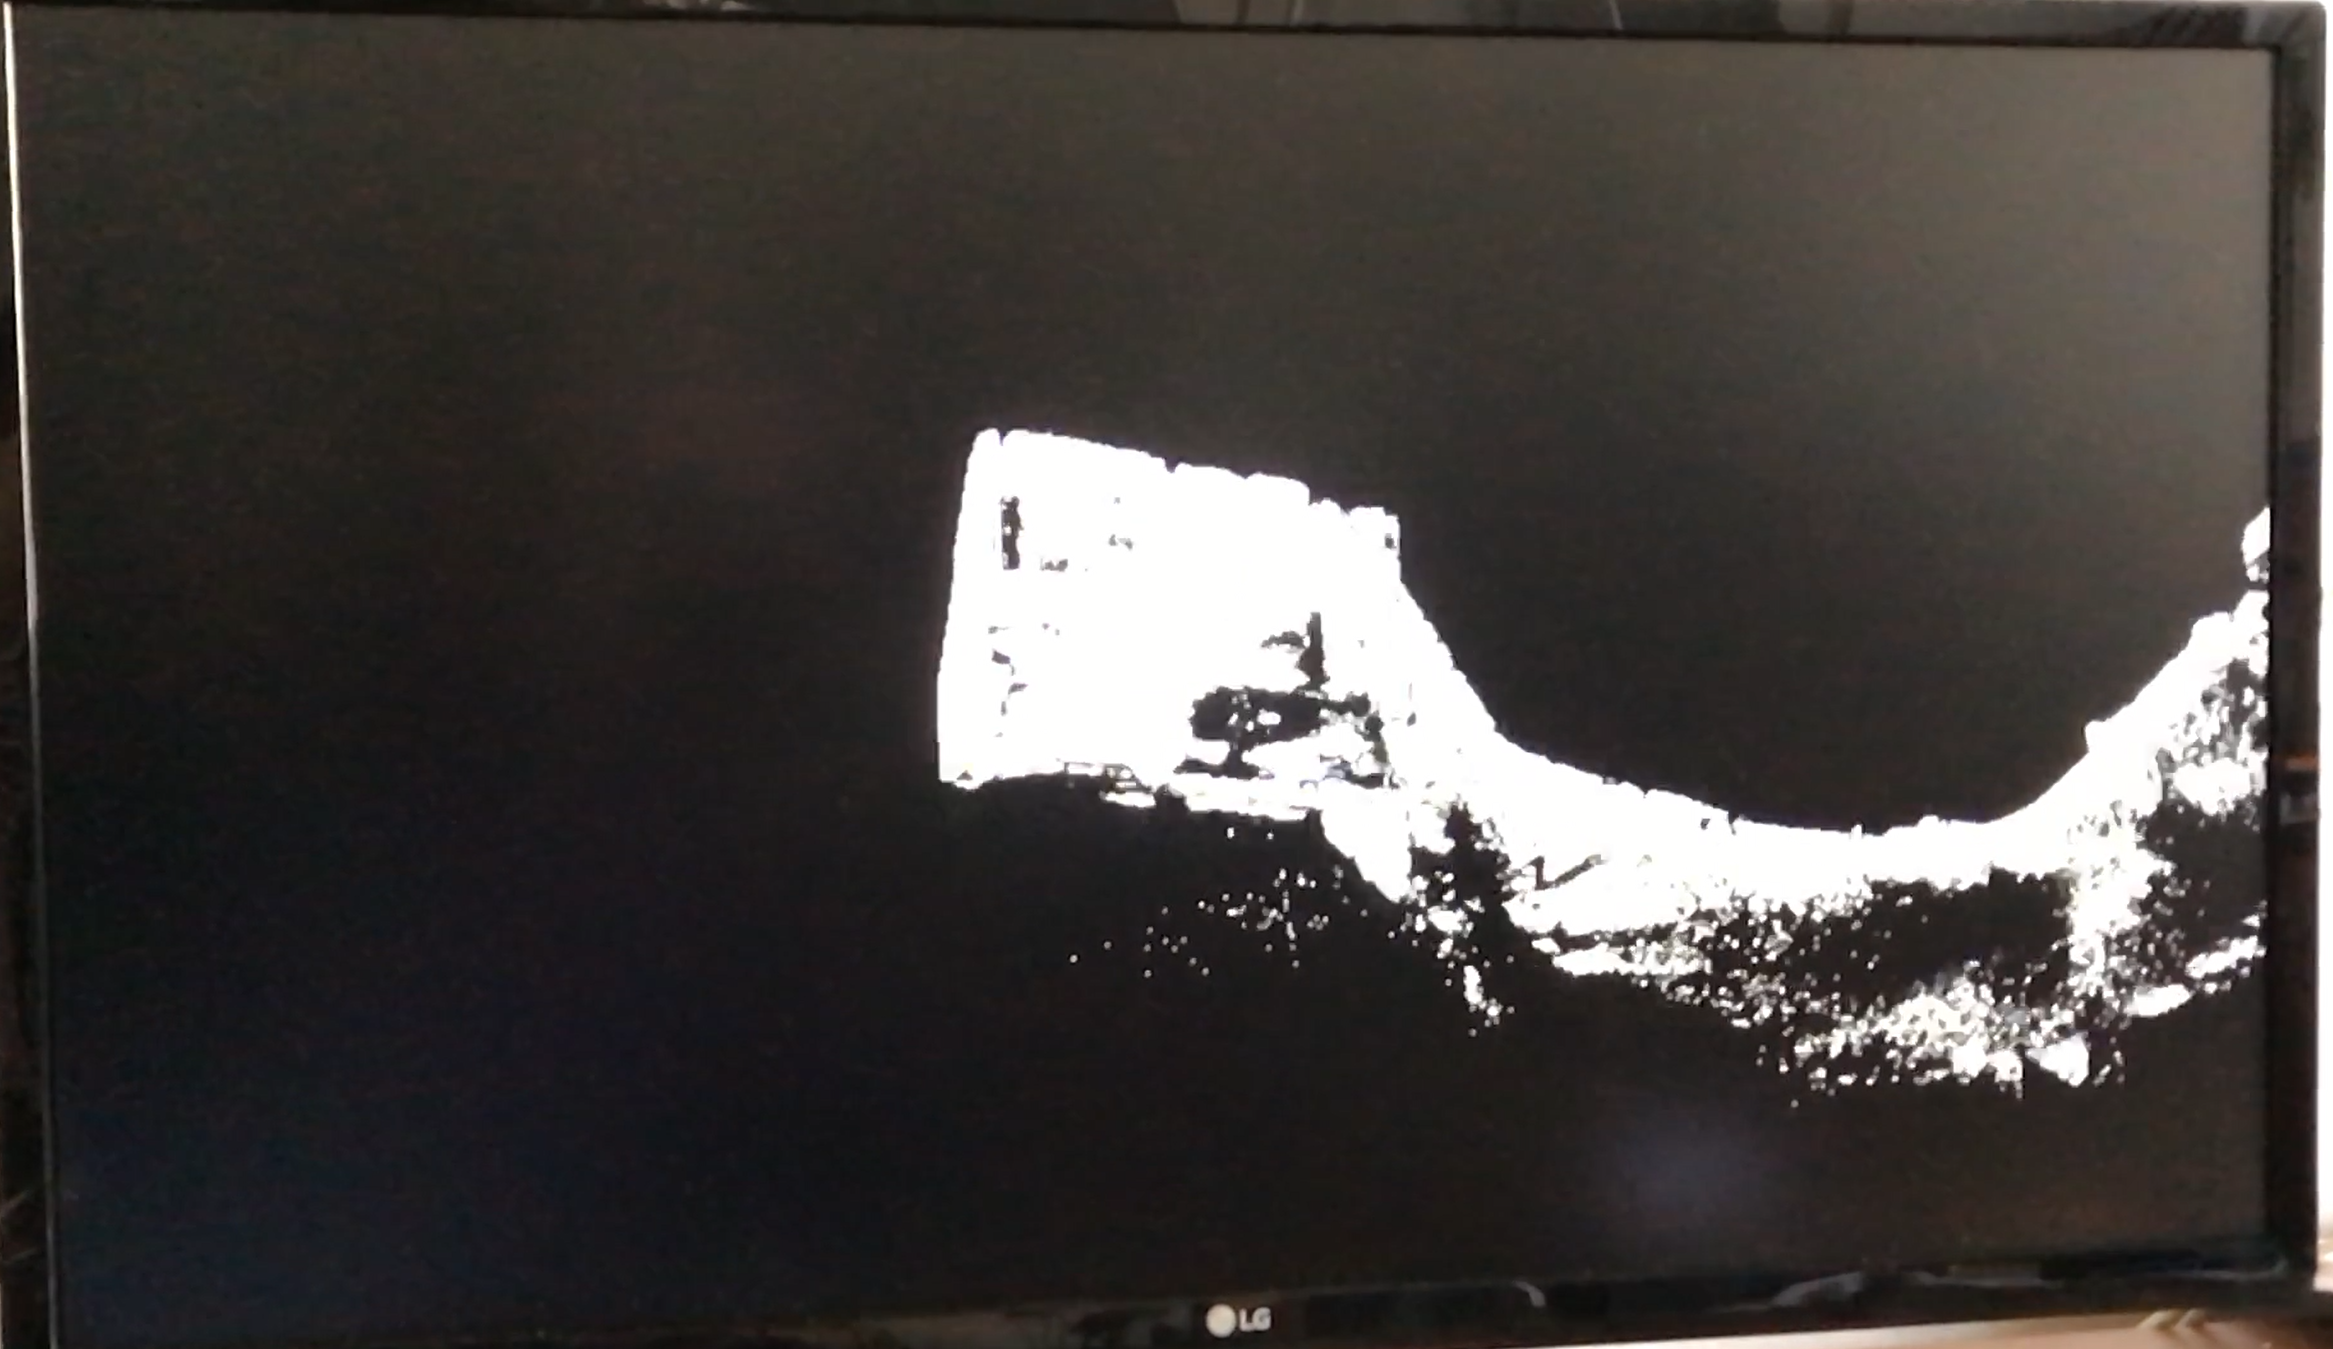
\includegraphics[scale=0.2]{img/4/vibe_example.png}
		\caption{Działający algorytm \textit{ViBE}}
		\label{fig:vibe_demo}
	\end{figure}	
	
	
\section{Implementacja rozszerzonej wersji ViBE}
\label{sec:fpga_vibe_plus}

W rozdziale \ref{subsec:vibe_ruchoma_kamera} opisany został dodatkowy mechanizm, usprawniający pracę algorytmu w przypadku występowania drgań kamery (ang. \textit{camera jitter}). Schemat implementacji rozszerzonej wersji algorytmu, zawierającej ten dodatkowy moduł, został przedstawiony na rysunku \ref{fig:vibe_plus_diagram}. Implementacja odpowiada opisowi teoretycznemu, który został przedstawiony w podrozdziale \ref{subsec:vibe_ruchoma_kamera}. Oprócz bloku realizującego standardowy algorytm \textit{ViBE}, opisanego szczegółowo w poprzednim rozdziale, ta wersja algorytmu zawiera także szereg modułów zapewniających prawidłowe przesunięcie modelu tła na podstawie wyznaczonego przepływu optycznego. Moduł, podobnie jak poprzednia wersja, wykorzystuje standardowy interfejs wizyjny, schemat modelu tła jest również identyczna jak w podstawowej wersji algorytmu. 
	
	\begin{figure}[h!]
		\centering
		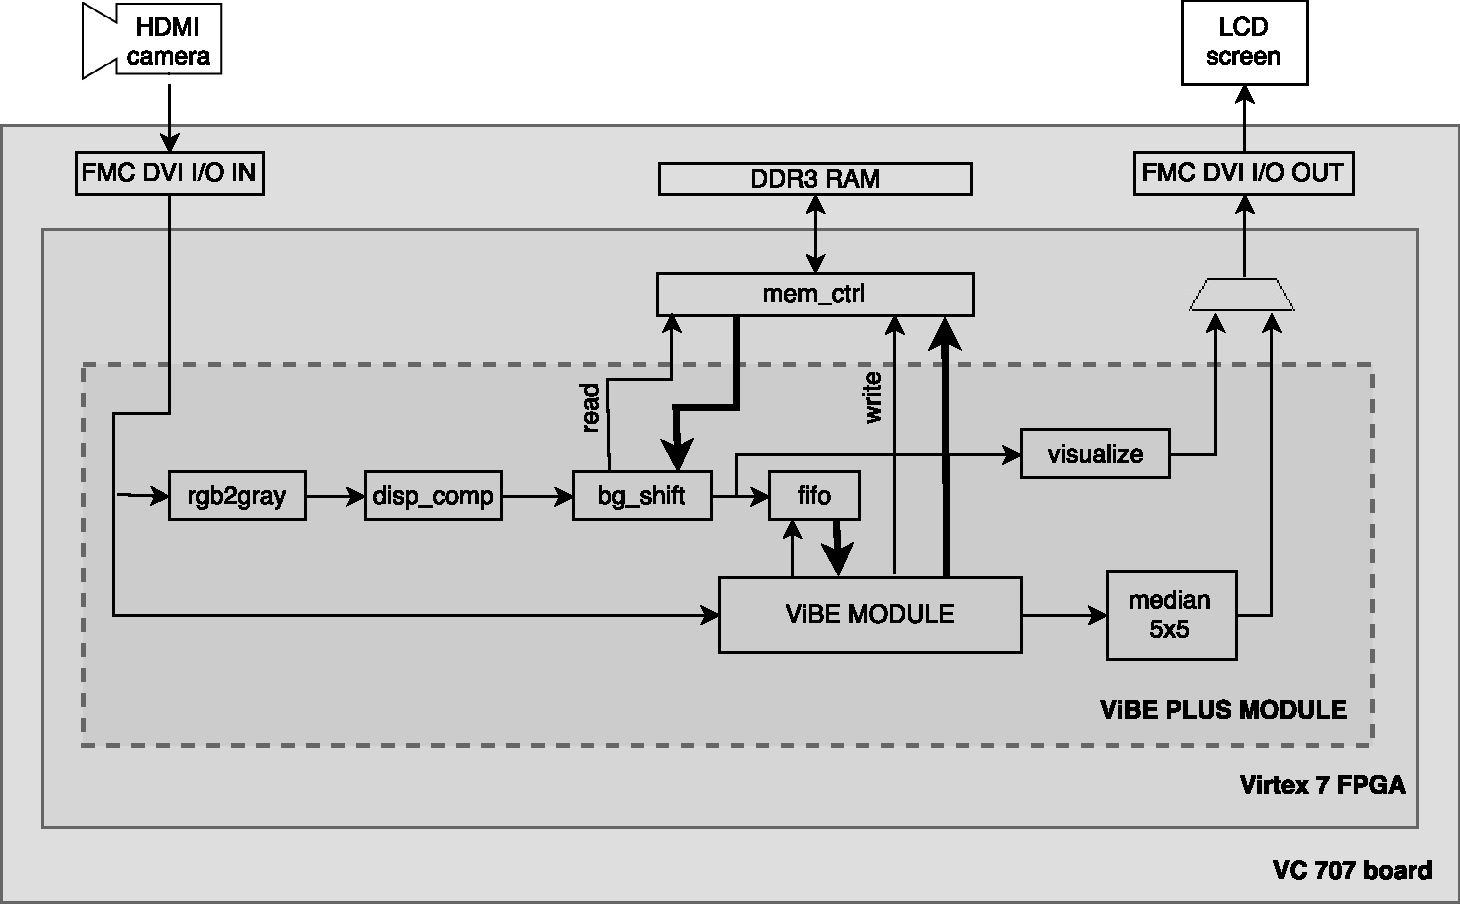
\includegraphics[scale=0.6]{img/4/vibe_plus.pdf}
		\caption{Wysokopoziomowy schemat implementacji rozszerzonego algorytmu \textit{ViBE}}
		\label{fig:vibe_plus_diagram}
	\end{figure}

Pierwszym krokiem, podczas obliczania przepływu optycznego, jest konwersja obrazu z przestrzeni \textit{RGB} do skali szarości. Jest to wykonywane poprzez moduł \textit{rgb2gray}. Przekształcony sygnał z kamery jest następnie podawany na wejście bloku \textit{disp\_comp}, realizującego operację wyznaczania przesunięcia modelu na podstawie wyliczonego przepływu optycznego. Jest to najbardziej złożony moduł w całej implementacji. Jego szczegółowy schemat został przedstawiony na rysunku \ref{fig:displacement_diagram}. Na podstawie otrzymanego wektora przesunięcia blok \textit{bg\_shift} zapewnia prawidłową synchronizację i odczyt kolejnych modeli tła z~pamięci \textit{RAM}. Ze względu na przesunięcie, operacja odczytu, musi zostać wykonana z odpowiednim wyprzedzeniem lub opóźnieniem. Dane z pamięci \textit{RAM} są umieszczane w kolejce \textit{FIFO} (ang. \textit{First In First Out} -- pierwszy na wejściu, pierwszy na wyjściu). Skąd następnie są pobierane przez algorytm \textit{ViBE}. Kolejka \textit{FIFO}, podobnie jak linie opóźniające, została zaimplementowana z wykorzystaniem pamięci blokowej (\textit{BRAM}). Dzięki zastosowaniu uniwersalnego interfejsu z niezależnymi sygnałami odczytu i~zapisu do pamięci RAM, nie było konieczności modyfikowania oryginalnej implementacji metody \textit{ViBE}. Na maskę wyjściową, nakładany jest filtr medianowy o rozmiarze $5x5$, dodatkowo został zaimplementowany moduł wizualizujący operację obliczania przepływu optycznego.

Rozszerzona wersja algorytmu operuje jedynie na rozdzielczości \textit{720x576}. Zastosowano identyczne parametry jak w podstawowej wersji metody, czyli model tła składający się z 20 próbek w przestrzeni \textit{CIELab}. Składowa wektora przesunięcia może przyjąć maksymalnie wartość $32$, zatem kolejka \textit{FIFO} gromadząca modele tła musi mieć długość $32 \cdot$\textit{H\_SIZE}$+32$, gdzie każdy element ma szerokość równą modelowi tła. Dla obsługiwanej rozdzielczości parametr \textit{H\_SIZE} wynosi 864, natomiast model tła ma rozmiar 460 bitów. Ostatecznie ustawiono szerokość pojedynczego elementu na 512 bitów, natomiast głębokość kolejki wynosi 32768.  

	\begin{figure}[h!]
		\centering
		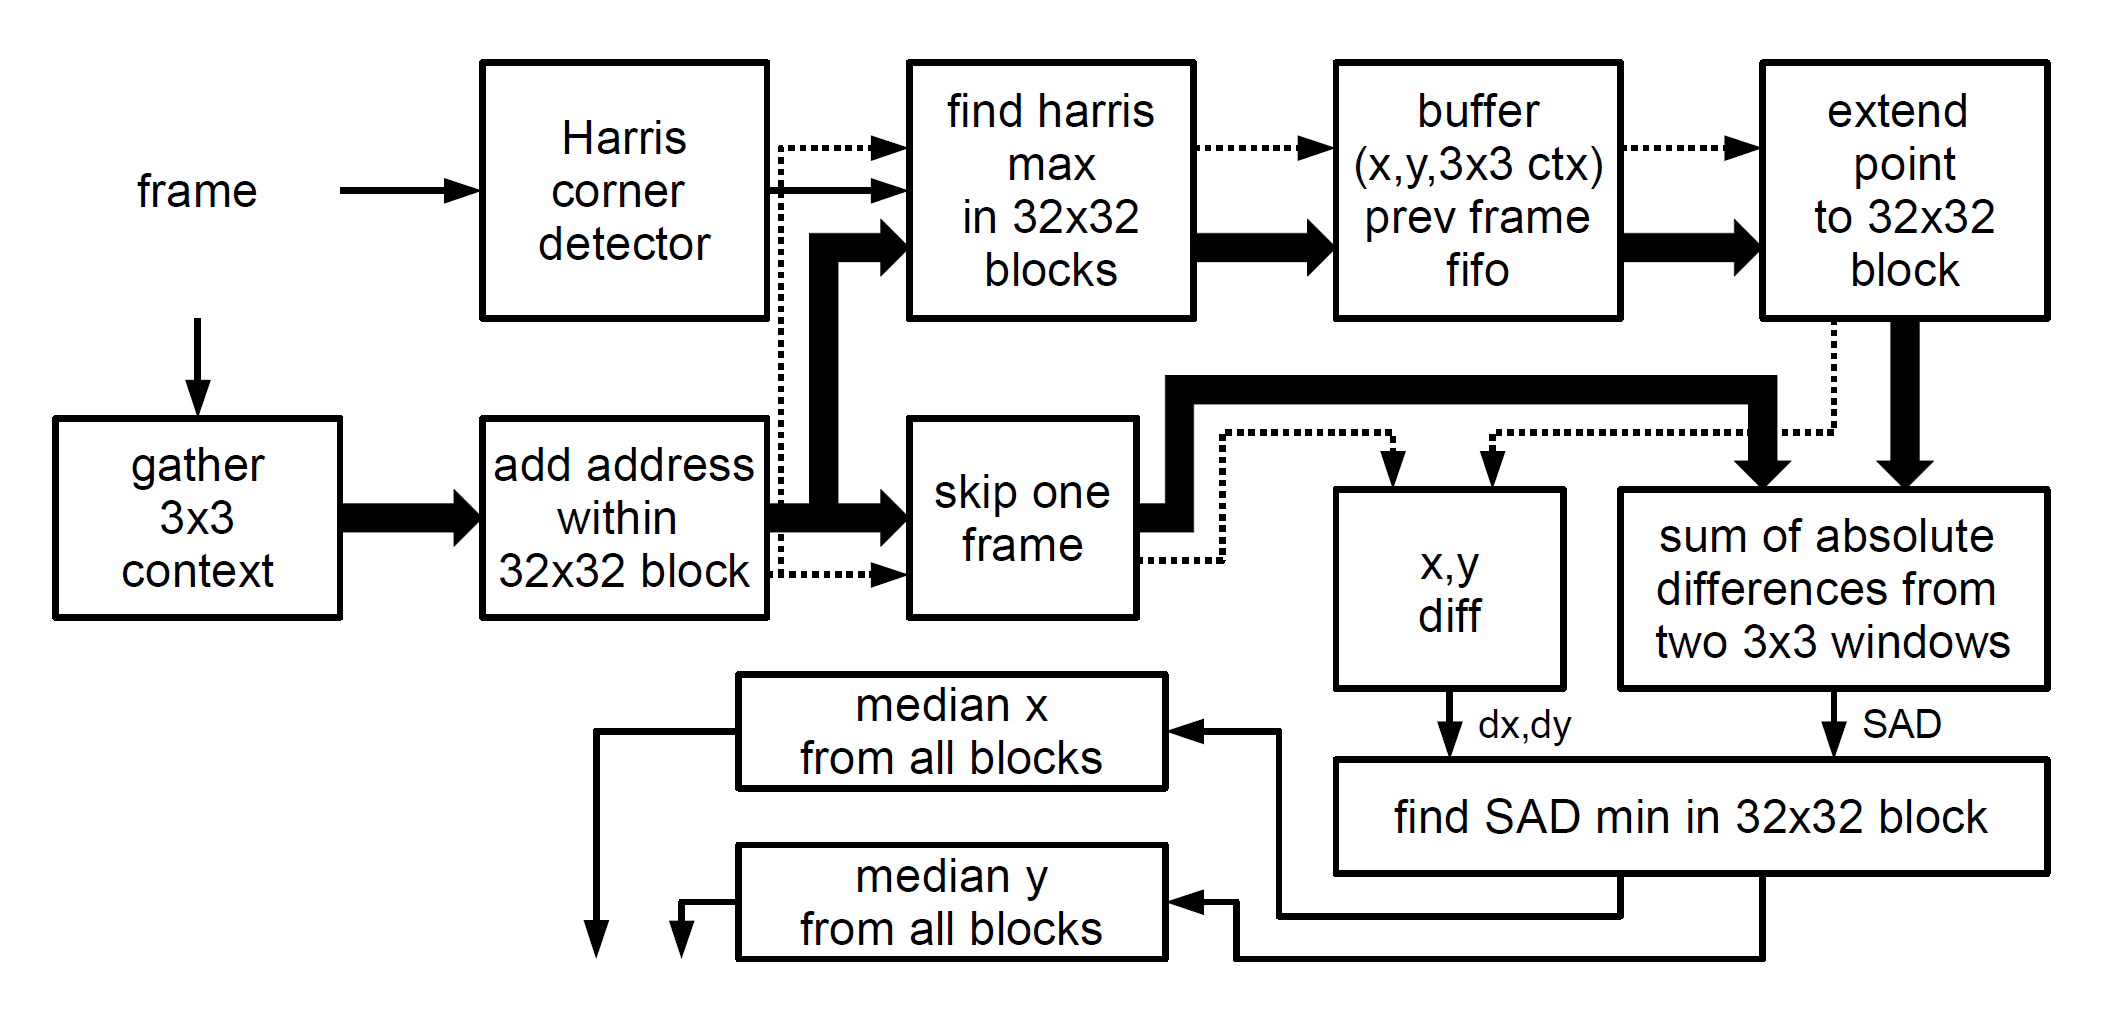
\includegraphics[scale=0.25]{img/4/displacement_vector_diagram.png}
		\caption{Implementacja modułu wyznaczającego wektor przesunięcia -- źródło \cite{}}
		\label{fig:displacement_diagram}
	\end{figure}

Moduł realizujący wyznaczanie wektora przesunięcia, jest najbardziej złożonym elementem algorytmu. Opis teoretyczny tej metody został przedstawiony w podrozdziale \ref{subsec:vibe_of}. pierwszym krokiem algorytmu jest detekcja narożników metodą Harrisa-Stephensa. Schemat przedstawiający implementację tej funkcji został pokazany na rysunku \ref{fig:harris_diagram}. Wykonane tam operacje odpowiadają opisowi teoretycznemu zamieszczonemu w podrozdziale \ref{subsec:vibe_harris}. Przy implementacji uwzględniono w maksymalnym stopniu możliwości układu FPGA w zakresie zrównoleglania obliczeń. Moduły \textit{prewitt\_x} i \textit{prewitt\_y} realizują detekcję krawędzi pionowych i poziomych. Następnie wszystkie trzy elementy macierzy $H$ są obliczane równolegle. Po dokonaniu operacji wygładzania filtrem Gaussa (blok \textit{gaussian\_blur}) w bloku \textit{rescaling} następuje przeskalowanie (dzielenie przez $2^10$) otrzymanych wartości. Finalnie wyznaczany jest wyznacznik macierzy $H$, zgodnie z równaniem (\ref{equ:vibe_harris_response_final}). Całość została zrealizowana z wykorzystaniem sprzętowych mnożarek i sumatorów. Konieczne jest wykonanie 6 operacji mnożenia, jednego dodawania i dwóch odejmowania.
 
	\begin{figure}[h!]
		\centering
		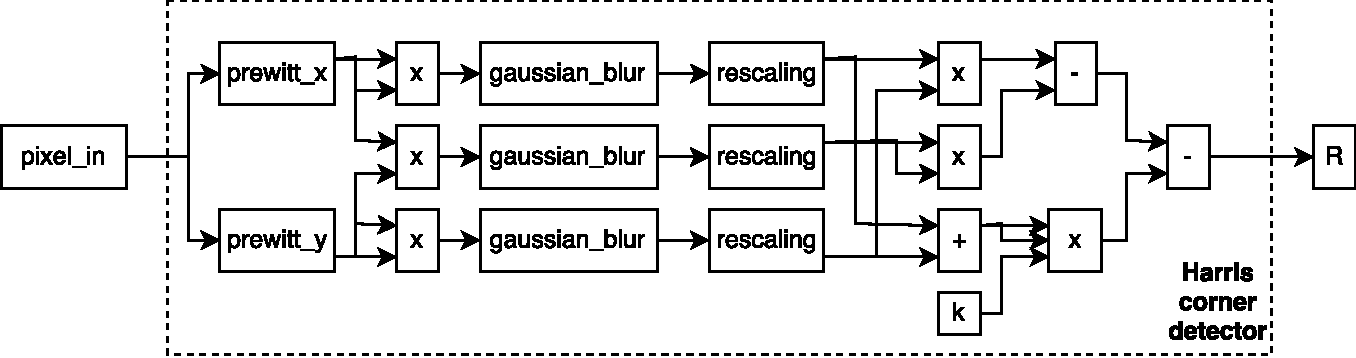
\includegraphics[scale=0.6]{img/4/harris_detector.pdf}
		\caption{Moduł realizujący detekcję narożników metodą Harrisa-Stephensa}
		\label{fig:harris_diagram}
	\end{figure}

Równolegle do detekcji krawędzi wyznaczany jest kontekst aktualnego piksela o rozmiarze $3x3$, określana jest także jego pozycja w aktualnie przetwarzanym bloku o rozmiarze $32x32$. Piksel dla którego otrzymano najmniejszą wartość współczynnika $R$ w obszarze każdego bloku zostaje zapisany razem z kontekstem $3x3$ w kolejce \textit{FIFO} (w przypadku obrazu o rozdzielczości \textit{720x576} konieczne jest zdefiniowanie kolejki o rozmiarze 396, gdyż tyle jest bloków $32x32$ w jednej ramce). Kolejne elementy z~kolejki, są pobierane w trakcie przetwarzania następnej ramki obrazu. W każdym z bloków znajdowana jest minimalna wartość sumy różnicy modułów pomiędzy pikselem pobranym z kolejki i pikselami z~aktualnej ramki obrazu. Znaleziona wartość, wraz z wektorem przesunięcia, zostaje po raz kolejny zapamiętana w pamięci blokowej. 

Ostatnim krokiem, jest obliczenie mediany przesunięcia $dx$ i $dy$ wśród znalezionych wartości minimalnych. Operacja ta, składa się z dwóch etapów, wykonywanych w momencie przerwy pomiędzy kolejnymi ramkami obrazu (wartość sygnału \textit{vsync} wynosi wtedy $0$). Najpierw wyliczany jest histogram wartości $dx$ i $dy$, równolegle zliczana jest także ilość próbek. Drugim krokiem jest sumowanie wartości histogramu. Poprzez mediane, rozumiemy wartość, dla której aktualna suma wartości histogramu jest większa niż połowa liczby wszystkich próbek. Do obliczenia histogramu ponownie został wykorzystany moduł pamięci blokowej (\textit{BRAM}). Na rysunku \ref{fig:vibe_plus_demo} przedstawiono wizualizację wyznaczanego przepływu optycznego, analogiczną do tej pokazanej na rysunku \ref{fig:vibe_of_example}.

	\begin{figure}[h!]
		\centering
		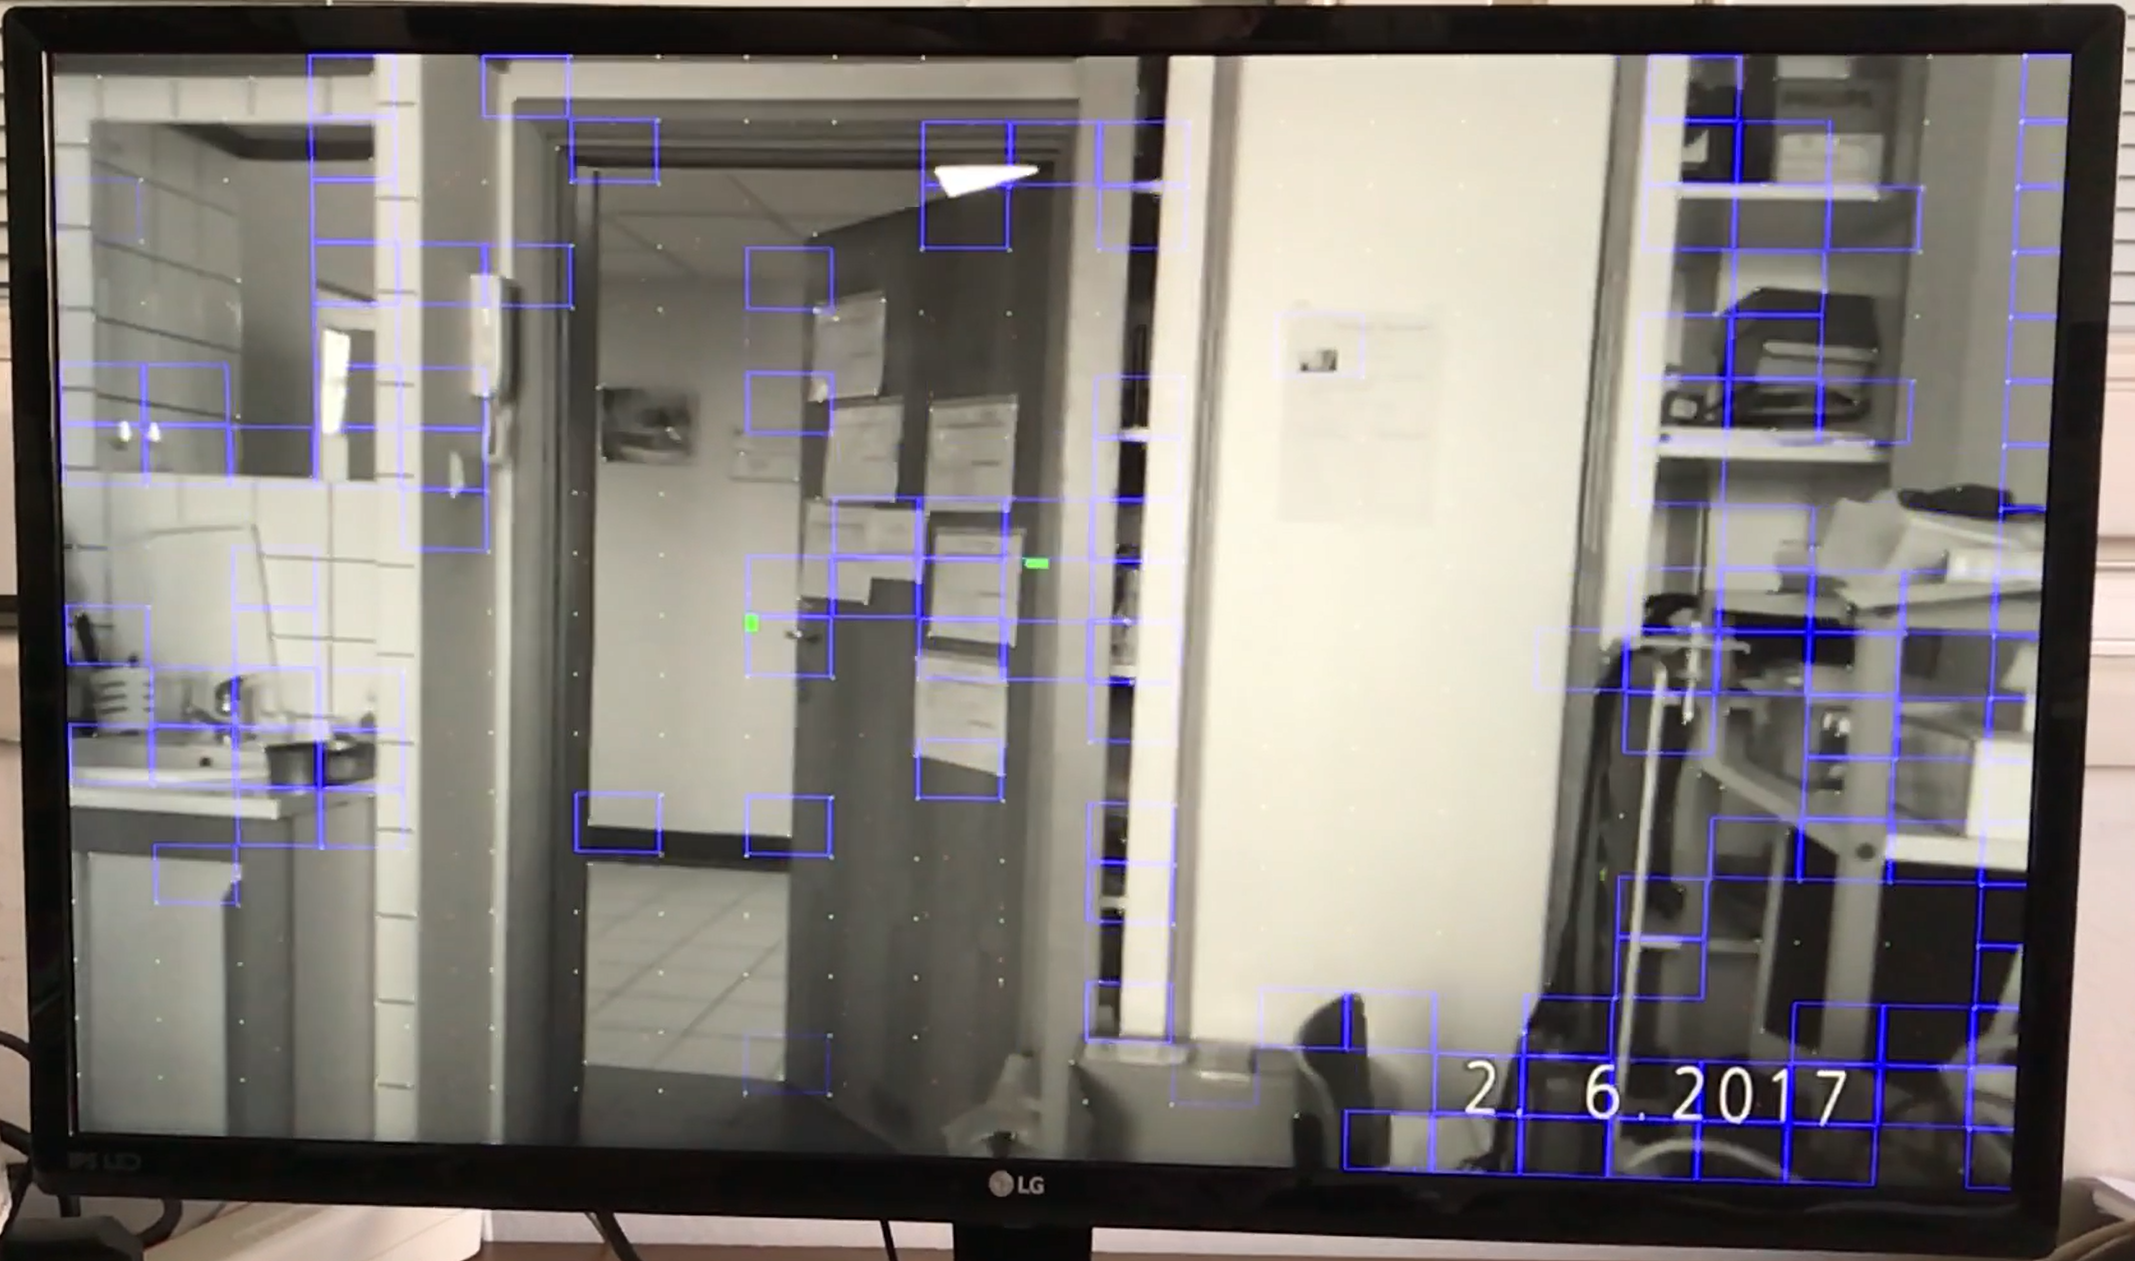
\includegraphics[scale=0.2]{img/4/vibe_plus_example.png}
		\caption{Wizualizacja przepływu optycznego}
		\label{fig:vibe_plus_demo}
	\end{figure}
	

\section{Implementacja algorytmu PBAS}
\label{sec:fpga_pbas}

Szczegółowy opis teoretyczny algorytmu \textit{PBAS} został zamieszczony w podrozdziale \ref{sec:pbas_teoria}. Zaimplementowano wariant operujący w przestrzeni kolorów \textit{RGB} w rozdzielczości \textit{720x576} pikseli oraz wersję przetwarzającą obraz w skali szarości, w przypadku wyższych rozdzielczości (\textit{720p} i \textit{1080p}). Wysokopoziomowy schemat całego algorytmu został przedstawiony na rysunku \ref{fig:pbas_diagram}. Jak zostało już wspomniane w części teoretycznej, wersja algorytmu działająca w przestrzeni \textit{RGB}, przetwarza niezależnie poszczególne składowe, tworząc dla każdej z nich osobny model tła. 
	
	\begin{figure}[h!]
		\centering
		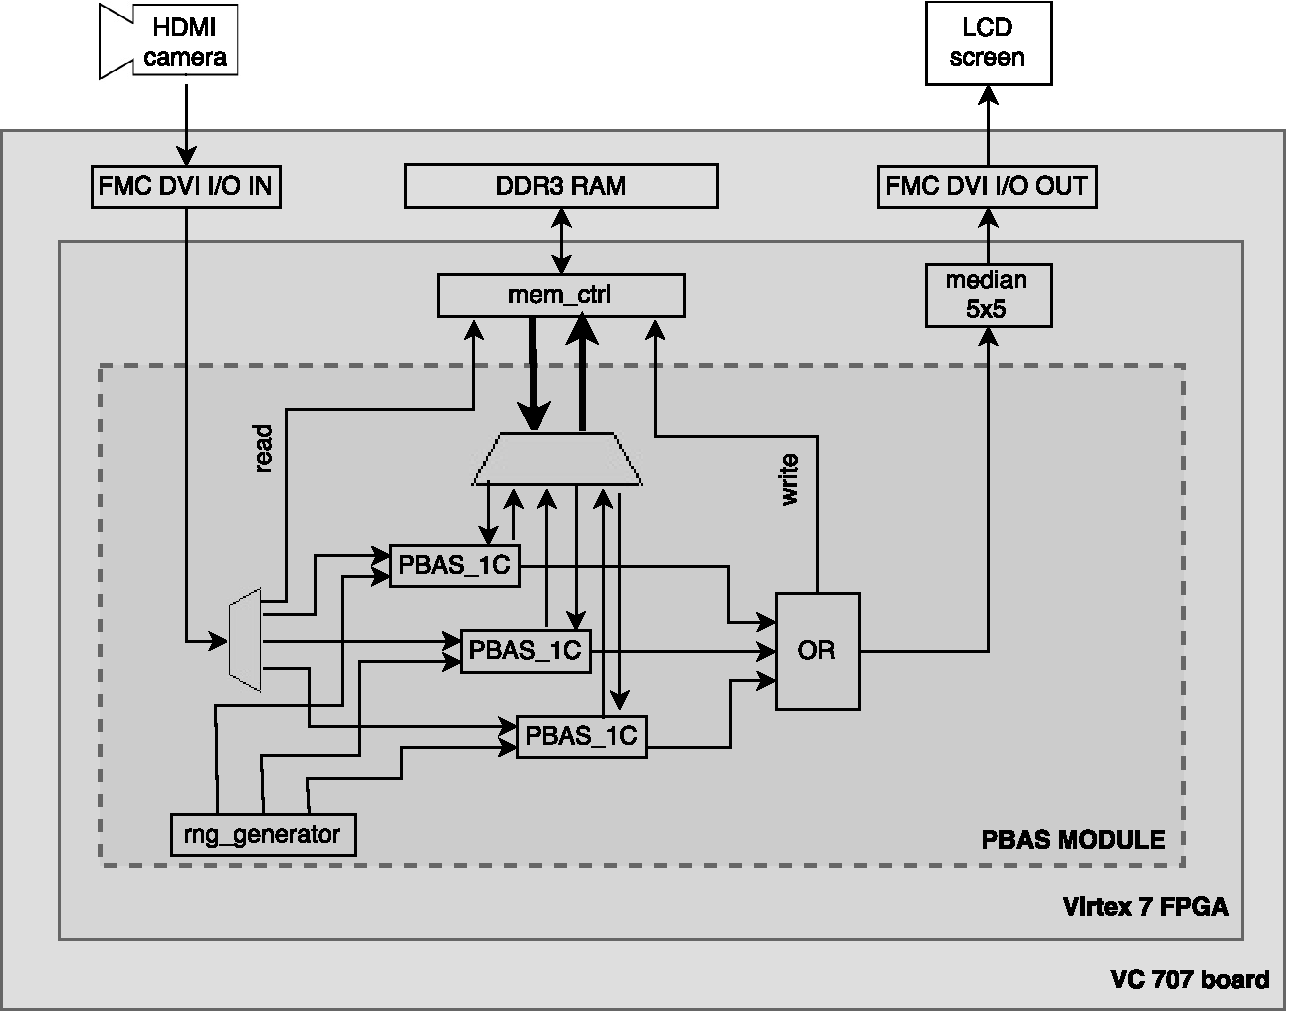
\includegraphics[scale=0.6]{img/4/pbas.pdf}
		\caption{Implementacja algorytmu \textit{PBAS} w wersji \textit{RGB}}
		\label{fig:pbas_diagram}
	\end{figure}

Pierwszą operacją, jest rozbicie sygnału wejściowego na składowe \textit{RGB}. Następnie każda z nich jest analizowana niezależnie poprzez algorytm \textit{PBAS} (blok \textit{PBAS\_1C}). Szczegółowy schemat implementacji modułu, realizującego algorytm dla jednej składowej, przedstawiono na rysunku \ref{fig:pbas_1c_diagram}. Maska finalna stanowi alternatywę logiczną wyników otrzymanych z poszczególnych modułów. Podobnie jak w przypadku innych algorytmów, tutaj także, na koniec, nakładany jest filtr medianowy w celu wyeliminowania szumów i zakłóceń. Algorytm wykorzystuje także generator liczb losowych, zaimplementowany w module \textit{rng\_generator}. Jego opis został szerzej przedstawiony w podrozdziale \ref{subsec:fpga_generator}. Opisywany moduł wykorzystuje oczywiście uniwersalny interfejs wizyjny przedstawiony w rozdziale \ref{sec:uklad_interfejs}. 
	
	\begin{figure}[h!]
		\centering
		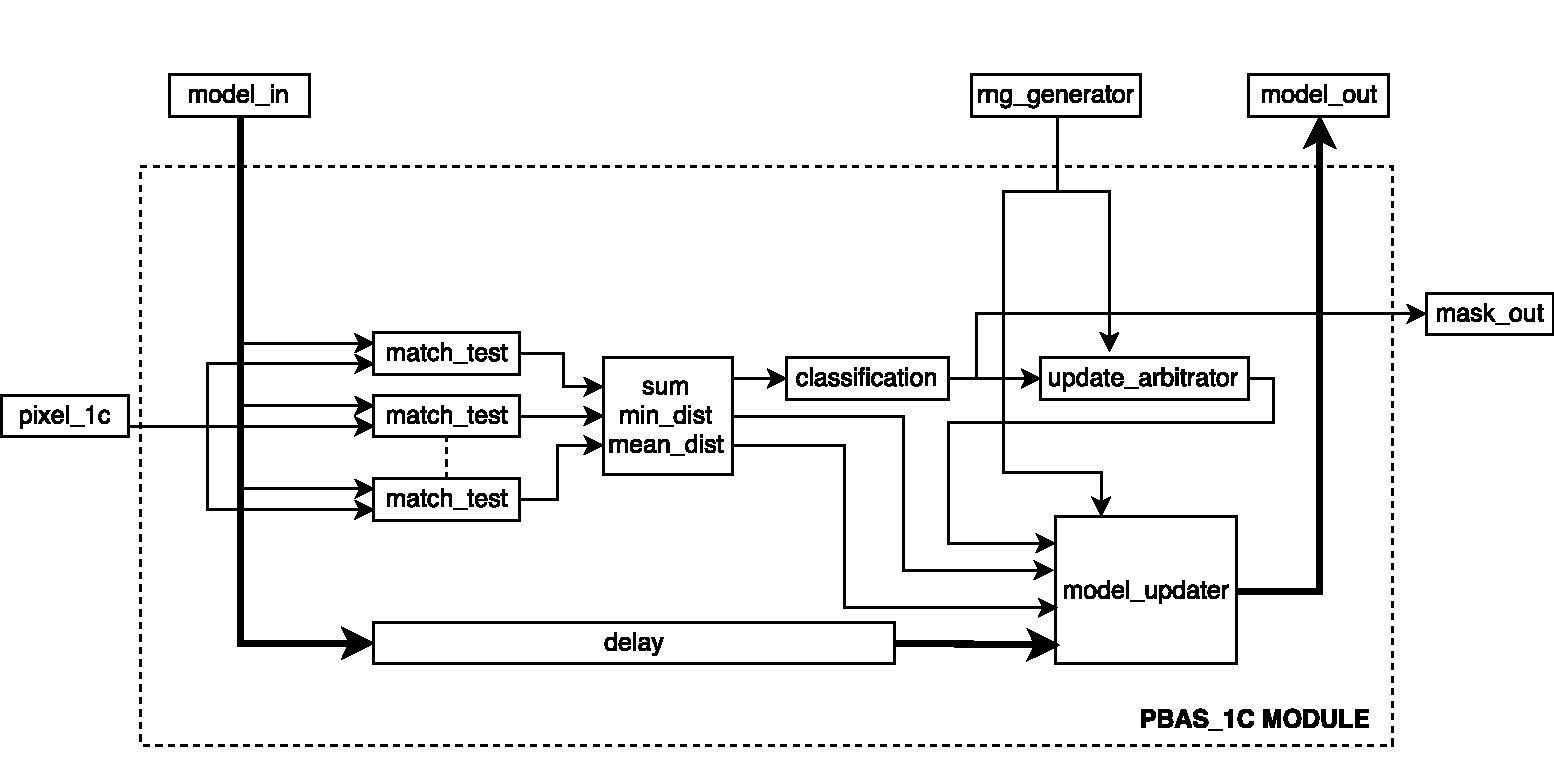
\includegraphics[scale=0.55]{img/4/pbas_1c.pdf}
		\caption{Implementacja algorytmu \textit{PBAS} dla jednej składowej \textit{RGB}}
		\label{fig:pbas_1c_diagram}
	\end{figure}	
	
Implementacja algorytmu \textit{PBAS} przedstawiona na rysunku \ref{fig:pbas_1c_diagram}, operującego na jednej składowej \textit{RGB} bądź skali szarości, jest bardzo podobna do implementacji metody \textit{ViBE} przedstawionej w rozdziale \ref{sec:fpga_vibe}. Podobnie jak w tamtym przypadku, tutaj także, pierwszym krokiem, jest równoległy test dopasowania do próbek zapisanych w pamięci \textit{RAM}, zgodnie z równaniem (\ref{equ:pbas_dist}). Następnie przeprowadzana jest klasyfikacja, opisana równaniem (\ref{equ:pbas_test}). Dodatkowo obliczany jest minimalny dystans pomiędzy próbkami z modelu a aktualnym pikselem oraz średnia wartość odległości zapisanych w modelu tła. Tak samo jak w metodzie \textit{ViBE}, decyzja o podjęciu aktualizacji realizowana jest przez moduł \textit{update\_arbitrator}. Blok dokonujący aktualizacji, jest rozszerzeniem tego co zostało zaprezentowane w implementacji metody \textit{ViBE}. Dodatkowo, oprócz próbek, aktualizowany jest także zbiór minimalnych odległości oraz parametry $R$ i $T$, zgodnie z równaniami (\ref{equ:pbas_r_update}) i (\ref{equ:pbas_t_update}).

Pierwsza część modelu składa się z $N$ próbek, każda próbka zawiera wartość piksela -- $B_i$ oraz zapamiętany minimalny dystans -- $D_i$ pomiędzy aktualną próbką a aktualną wartością piksela. Na końcu znajdują się parametry $R$ i $T$. Modele dla poszczególnych składowych \textit{RGB} ustawione kolejno po sobie. Dla rozdzielczości \textit{576p} przyjęto model składający się z $N=19$ próbek. Parametry $R$ i $T$ zapisano w postaci 16-bitowych liczb stałoprzecinkowych w formacie \textit{8z8u}. Minimalny dystans, podobnie jak próbka, zapisana jest jako 8-bitowa liczba całkowita. Sumarycznie model tła dla jednej składowej \textit{RGB} ma rozmiar $19 \cdot (8+8) + 16 + 16 = 336$ bitów, zatem cały model zajmuje $3 \cdot 336 = 1008$ bitów. Dla wyższych rozdzielczości wykorzystano algorytm operujący na obrazie w skali szarości, model w tym przypadku składa się z $N=14$ próbek. Zatem, cały model, można zapisać za pomocą $14 \cdot (8+8) + 16 + 16 = 256$, jest to maksymalna szerokość modelu, która może zostać wykorzystana w przypadku obrazu w rozdzielczości \textit{720p} lub \textit{1080p}. 


\section{Implementacja rozszerzonej wersji metody PBAS}
\label{sec:fpga_pbas_plus}

Przedstawiona implementacja, powstała na podstawie opisu teoretycznego, zamieszczonego w rozdziale \ref{subsec:pbas_duchy}. Opisana tutaj, rozszerzona wersja algorytmu \textit{PBAS}, zawiera dodatkowy mechanizm rozróżniania obiektów statycznych od tzw. ,,duchów''. Koncepcja ta, wymaga także zaimplementowania metody indeksacji obiektów, co sprawia, że omawiany moduł jest najbardziej złożonym spośród wszystkich pokazanych w niniejszej pracy. Fragmenty przedstawionego tutaj rozwiązania pochodzą z publikacji \cite{kryjak_14_pbas}, również powstałej w Laboratorium Biocybernetyki AGH. Ogólny schemat przedstawiający architekturę modułu pokazano na rysunku \ref{fig:pbas_plus_diagram}. 
	
	\begin{figure}[h!]
		\centering
		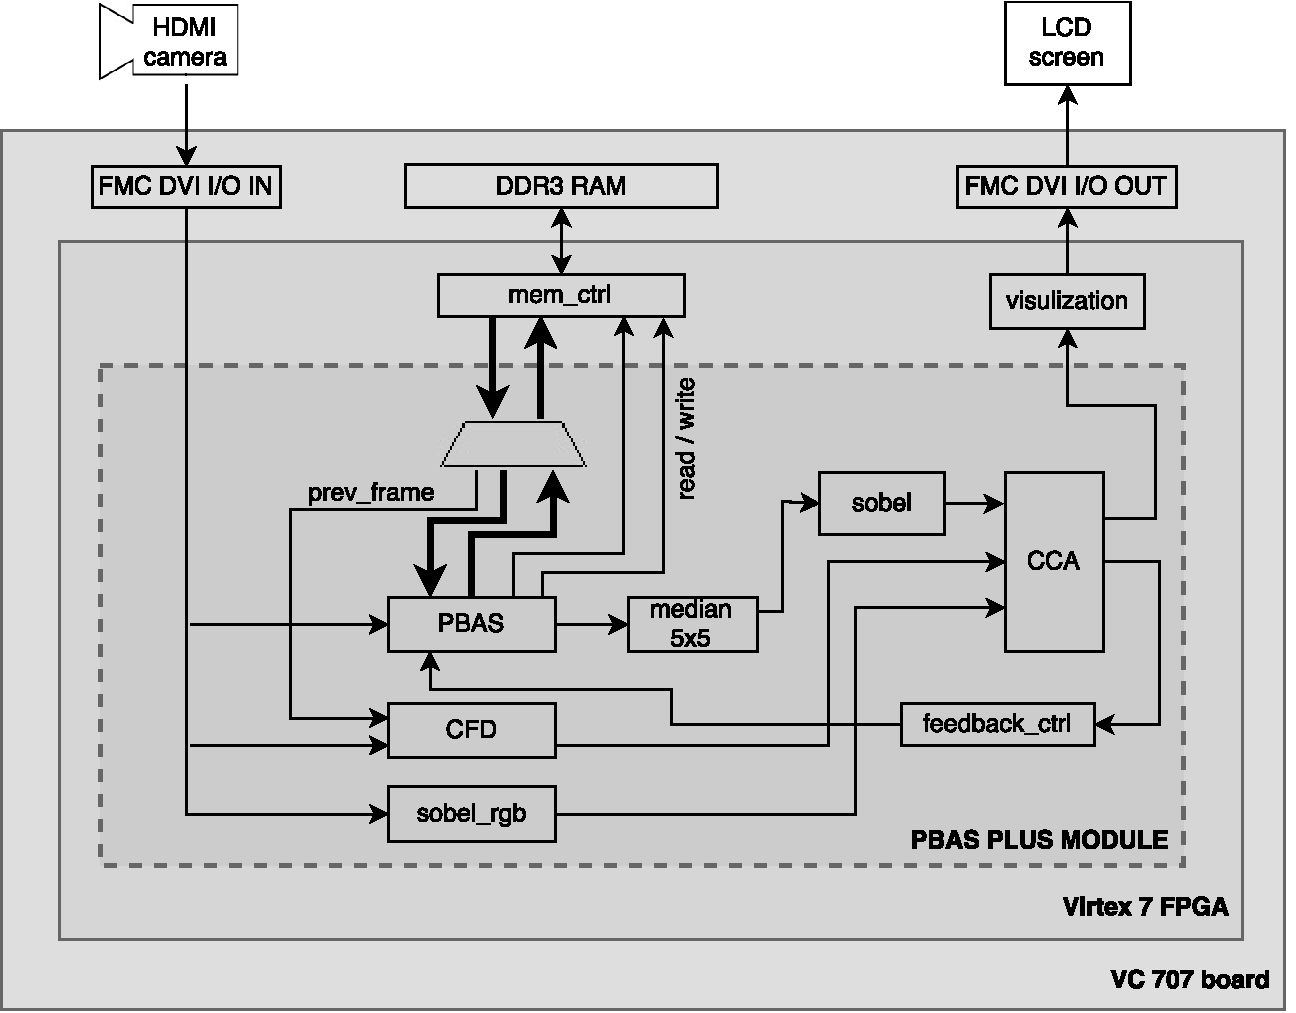
\includegraphics[scale=0.6]{img/4/pbas_plus.pdf}
		\caption{Implementacja rozszerzonej wersji algorytmu \textit{PBAS}}
		\label{fig:pbas_plus_diagram}
	\end{figure}
	
Pierwszym istotnym elementem jest realizacja podstawowego algorytmu \textit{PBAS}, w stosunku do wersji przedstawione w rozdziale \ref{} musiał on zostać zmodyfikowany. Konieczne było dodanie obsługi sprzężenia zwrotnego zgodnie z równaniami (\ref{}) i (\ref{}). Oprócz tego należało także zapewnić aktualizację dwóch nowych parametrów $S(x_i)_{cnt}$ i $E(x_i)_{mean}$, zgodnie z równaniami (\ref{equ:pbas_s_cnt}) i (\ref{equ:pbas_ec_mean}). Dodatkowo w modelu tła musi znaleźć się też poprzednia wartość piksela ($24$ bity) wykorzystywana podczas odejmowania ramek (blok \textit{CFD}). W związku z tym, aby rozmiar modelu nie przekroczył maksymalnego rozmiaru wynoszącego $1024$ bity, konieczne było zredukowanie liczby próbek w algorytmie \textit{PBAS} do $18$. Parametr $S(x_i)_{cnt}$ zapisany jest jako 8 bitowa liczba całkowita, z kolei wartość $E(x_i)_{mean}$ to 16 bitowa liczba stałoprzecinkowa w formacie \textit{8z8u}. Ostatecznie rozmiar modelu tła w takiej konfiguracji wynosi: $3 \cdot (18 \cdot (8+8) + 16 + 16) + 8 + 16 + 24 = 1008$ bitów.

Równolegle do algorytmu \textit{PBAS} wykonywane jest, wspomniane wcześniej, odejmowanie ramek oraz detekcja krawędzi metodą Sobela. Na maskę wyjściową podobnie jak w poprzednich metodach, nakładany jest filtr medianowy. Wyznaczane są także krawędzie na masce binarnej, gdyż jest to niezbędne podczas przeprowadzania analizy poszczególnych obiektów. Schemat bloku \textit{CCA}, odpowiedzialnego za to zadanie, został pokazany na rysunku \ref{fig:cca_diagram}. Ze względu ma fakt, że dane z modułu analizy obiektów dostępne są dopiero po przetworzeniu całej ramki obrazu, konieczne jest zapewnienie odpowiedniej synchronizacji sygnałów sprzężenia zwrotnego z modułem  \textit{PBAS}. Zadanie to zostało zrealizowane poprzez blok \textit{feedback\_ctrl}. Wyznaczone wartości współczynników stabilności i podobieństwa krawędzi oraz finalna maska są zapisywane w pamięci \textit{BRAM}. Działający algorytm, poprawnie identyfikujący obiekt pierwszoplanowy oraz prostokąt go otaczający, został pokazany na rysunku \ref{fig:pbas_plus_demo}.

	\begin{figure}[h!]
		\centering
		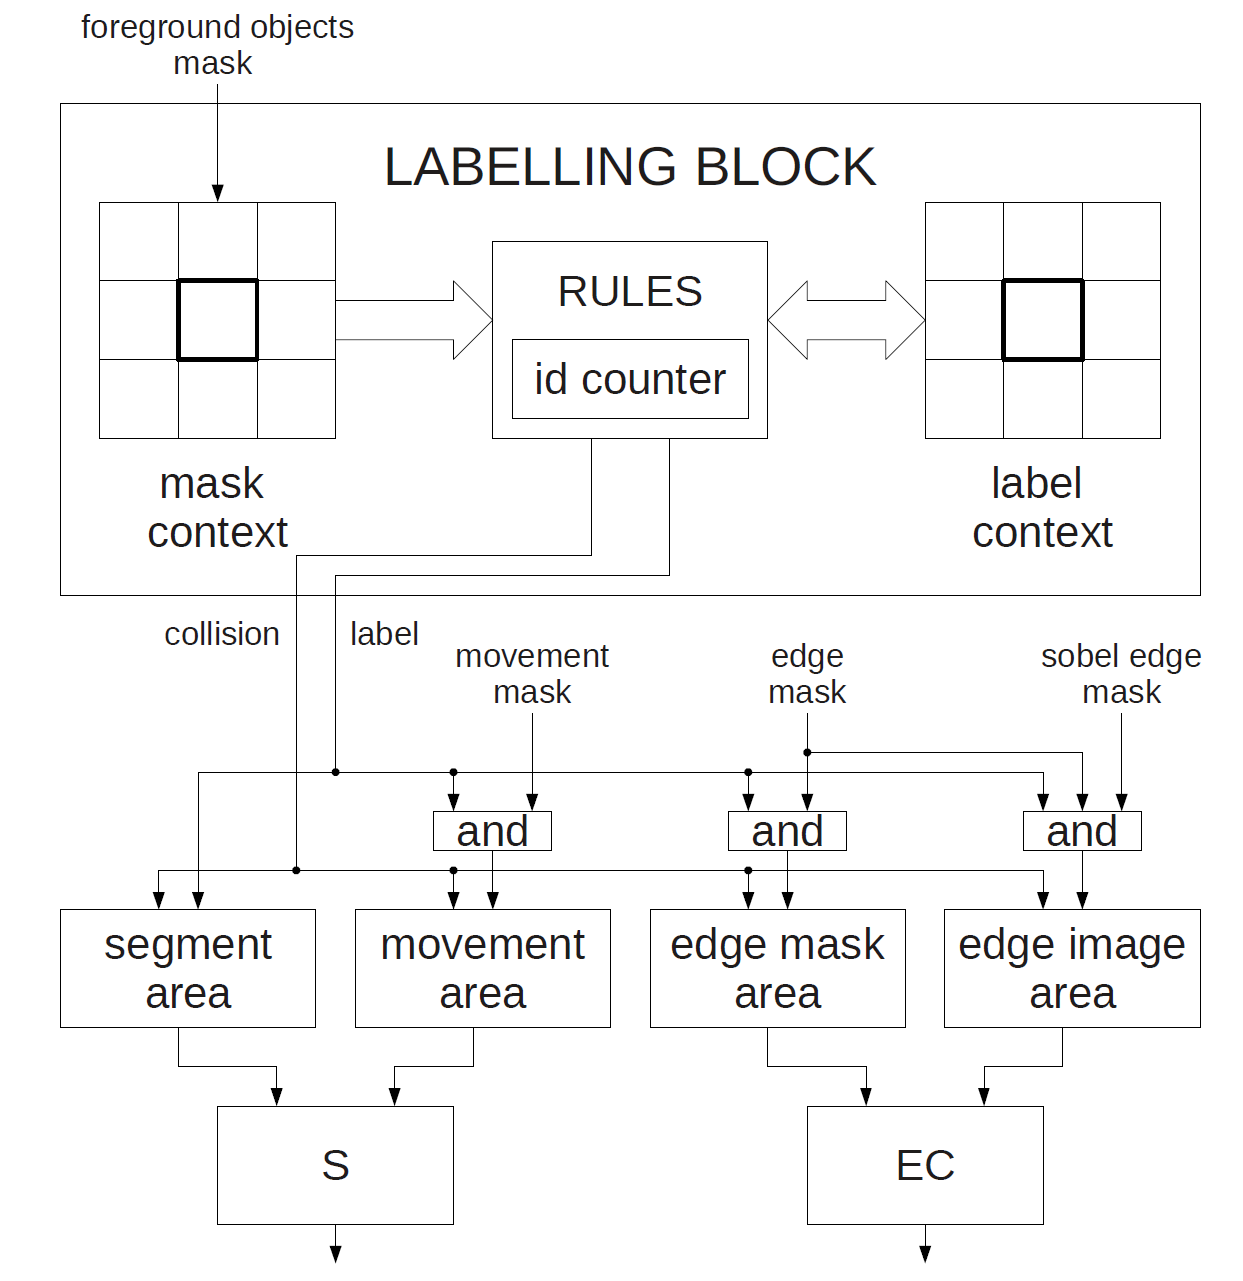
\includegraphics[scale=0.35]{img/4/cca_diagram.png}
		\caption{Architektura modułu \textit{CCA} -- źródło \cite{kryjak_14_pbas}}
		\label{fig:cca_diagram}
	\end{figure}

Do zrealizowania zadania indeksacji obiektów wykorzystano moduł \textit{CCA} opracowany w ramach publikacji \cite{kryjak_14_pbas}. Całość została przygotowana w oparciu o teorię na temat indeksowania obiektów, przedstawioną w rozdziale \ref{subsec:pbas_indeksacja}. Przygotowany moduł składa się z dwóch części, pierwszą z nich jest fragment logiki programowej (\textit{Labelling Block}), odpowiedzialny za przypisanie kolejnym pikselom odpowiednich etykiet. Jak zostało to opisane w części teoretycznej, etykieta jest dobierana na podstawie sąsiednich pikseli oraz etykiet im przypisanych. Konieczne jest zatem wygenerowanie kontekstu piksela wejściowego, zawierającego etykiety przypisane sąsiadom.

Informacja o przydzielonej etykiecie przekazywana jest do czterech bloków obliczających pole zidentyfikowanego obiektu. Pierwszy licznik (\textit{segment area} służy do wyznaczenia całkowitego pola obiektu. Drugi moduł (\textit{movement area}) zlicza natomiast jedynie ruchome piksele. Wartości te są używane do wyznaczenia współczynnika $S_{O_k}$ zgodnie z równaniem \ref{equ:pbas_stability}, wykorzystano w tym celu dzielarkę sprzętową. Kolejny licznik (\textit{edge mask area}) służy do zliczania pikseli na pierwszoplanowej masce krawędzi. Ostatni z modułów (textit{edge image area}) wyznacza liczbę pikseli znajdujących się na wspomnianej wyżej masce oraz na zbinaryzowanym obrazie krawędzi obrazu wejściowego. Te dwie wartości służą do wyznaczenia parametru $EC_{O_k}$, zgodnie z równaniem \ref{equ:pbas_edge_coef}. Podobnie jak w poprzednim przypadku, tutaj także wykorzystano dzielarkę sprzętową.

Oprócz wymienionych czterech istnieje jeszcze jeden blok, aktualizujący na bieżąco parametry prostokąta otaczającego poszczególne obiekty. Wszystkie liczniki zostały zaimplementowane z użyciem pamięci blokowej \textit{BRAM}. Problem konfliktów rozwiązano, poprzez sumowanie wartości zapamiętanych dla obu łączonych obiektów i zapisanie jej jako nowej wartości dla obiektu o niższej etykiecie. Wartość zapisana pod adresem wyższej etykiety zostaje natomiast oznaczona jako nieważna.

	\begin{figure}[h!]
		\centering
		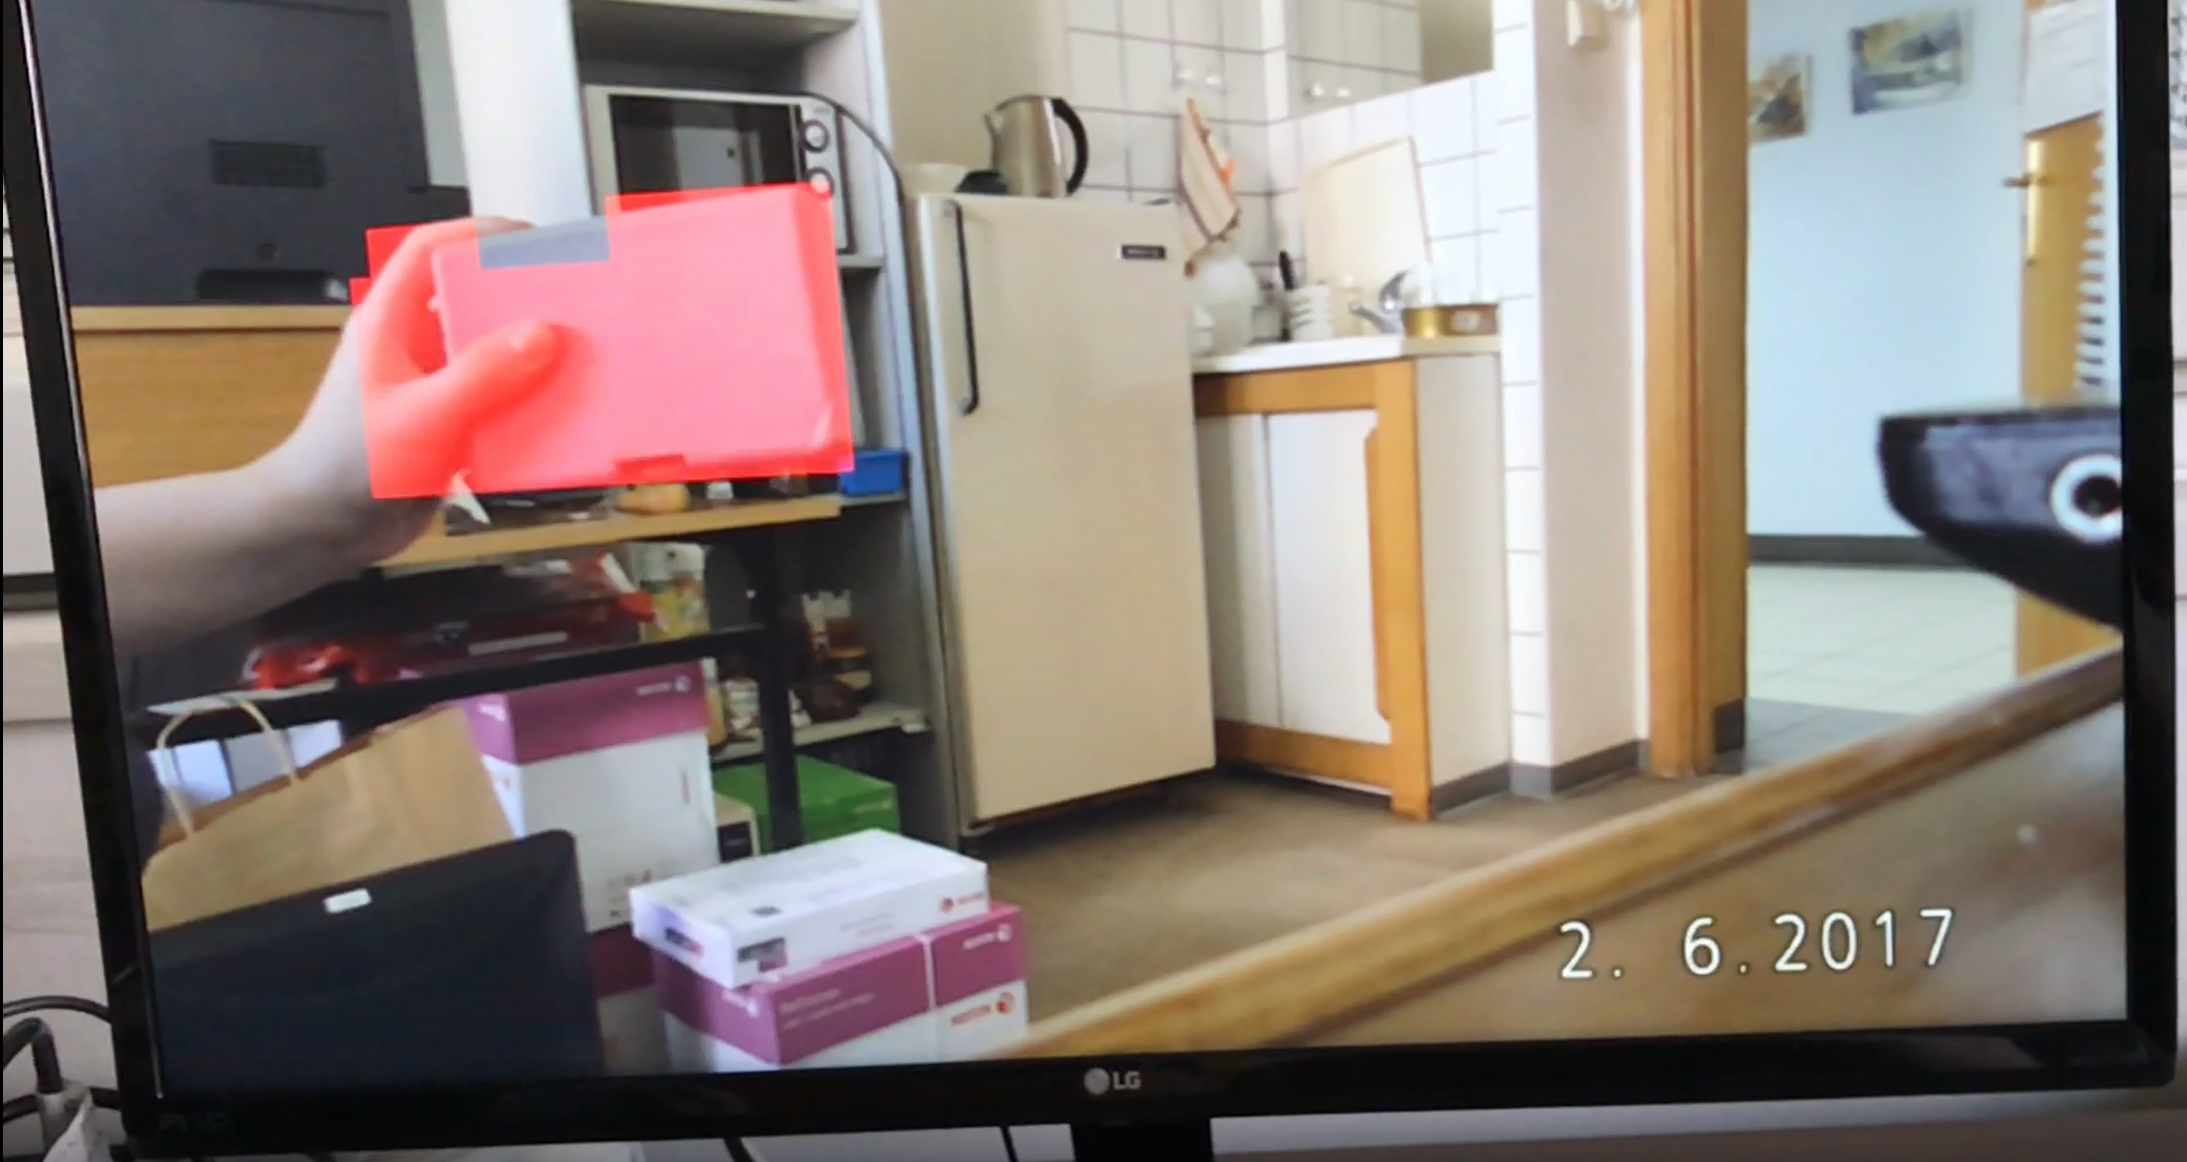
\includegraphics[scale=0.2]{img/4/pbas_plus_example.png}
		\caption{Działający algorytm \textit{PBAS} wraz z indeksacją obiektów}
		\label{fig:pbas_plus_demo}
	\end{figure}

\section{Implementacja GMM}
\label{sec:fpga_gmm}

Przedstawiona tutaj implementacja algorytmu \textit{GMM} została przygotowana w ramach pracy inżynierskiej \cite{piszczek_15}. Sposób implementacji sprzętowej omawianej metody jest tematem niezwykle rozległym, w niniejszym rozdziale przedstawiono jedynie ogólną idee przygotowanej architektury bez zagłębiania się w szczegóły implementacyjne. Schemat przedstawiający implementację i wykorzystane moduły został pokazany na rysunku \ref{fig:gmm_diagram}.

	\begin{figure}[h!]
		\centering
		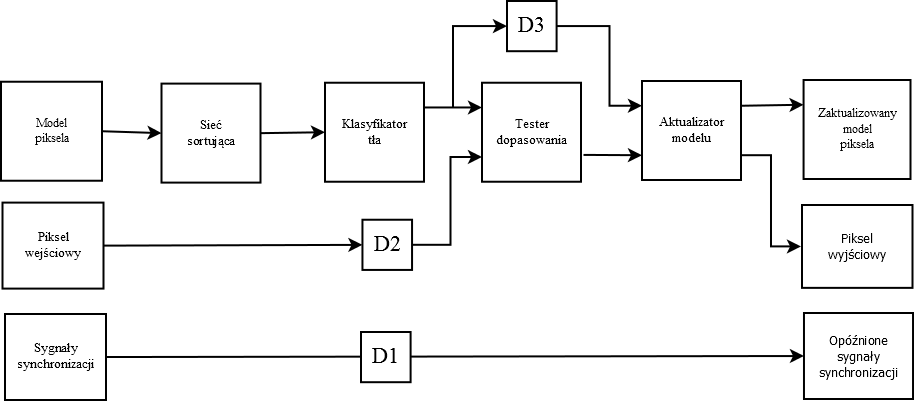
\includegraphics[scale=0.45]{img/4/gmm.png}
		\caption{Implementacja algorytmu \textit{GMM} -- źródło \cite{piszczek_15}}
		\label{fig:gmm_diagram}
	\end{figure}
	
Niewątpliwą zaletą, znacząco ułatwiającą implementację w układzie reprogramowalnym jest brak operacji kontekstowych. Dzięki temu możemy znacząco uprościć logikę programową i zredukować zużycie zasobów. Nawiązując do opisu teoretycznego zamieszczonego w rozdziale \ref{sec:gmm_teoria}, pierwszym krokiem algorytmu jest sortowanie rozkładów Gaussa według współczynnika $r_i = \frac{\omega_i}{\sigma_i}$. W tym celu wykorzystana została specjalnie zaprojektowana sieć sortująca, jest to najbardziej złożony element przedstawianej implementacji. 

Po dokonaniu sortowania, poszczególne rozkłady Gaussa są klasyfikowane, na podstawie równania \ref{equ:gmm_b}. Następnie przeprowadzany jest test dopasowania i ostateczna klasyfikacja piksela, zgodnie z~równaniem \ref{equ:gmm_mahalanobis}. Po dokonaniu klasyfikacji rozkłady Gaussa są aktualizowane i zapisywane w pamięci \textit{RAM}.

Przygotowana implementacja przetwarza obraz we wszystkich wymaganych rozdzielczościach, czyli \textit{576p}, \textit{720p} i \textit{1080p} w 50 klatkach na sekundę. Dla obrazu \textit{720x576} przyjęto $K=5$ rozkładów Gaussa w każdym model, natomiast dla wyższych rozdzielczości, ze względu na ograniczenia pamięci \textit{RAM}, liczba rozkładów wynosi $K=3$. W modelu tła pojedynczy rozkład Gaussa ma rozmiar $68$ bitów, dokładny opis i reprezentacja poszczególnych bitów modelu została przedstawiona w tabeli \ref{tab:gmm_ram_model}.

\begin{table}[h]
	\centering
	\begin{threeparttable}
		\caption{Znaczenie kolejnych bitów w reprezentacji rozkładu Gaussa -- źródło \cite{piszczek_15}}
		\label{tab:gmm_ram_model}

		\begin{tabular}{| c | m{12.5cm} |}  
		\hline
		\textbf{Zakres bitowy} & \multicolumn{1}{c|}{\textbf{Oznaczenie}} \\
		\hline
		\textit{0} & Bit pierwszego planu. Jeśli jest równy 1 oznacza to, że rozkład Gaussa reprezentuje obiekty pierwszoplanowe, w przeciwnym razie reprezentuje on tło. \\
		\hline
		\textit{1 -- 7} & Bity zarezerwowane (w razie wprowadzenia nowych flag). \\
		\hline
        \textit{8 -- 19} & Waga rozkładu Gaussa $\omega$ jako liczba stałoprzecinkowa (zakres 0 -- 1). Część całkowita zajmuje 0 bitów, część ułamkowa 12 bitów. \\
	    \hline
	    \textit{20 -- 31} & Wariancja ($\sigma^2$) jako liczba stałoprzecinkowa (zakres 0 -- 256). Część całkowita zajmuje 8 bitów, część ułamkowa 4 bity. \\
	    \hline
	    \textit{32 -- 43} & Średnia wartość barwy czerwonej piksela jako liczba stałoprzecinkowa (zakres 0 -- 256). Część całkowita zajmuje 8 bitów, część ułamkowa 4 bity. \\
        \hline
        \textit{44 -- 55} & Średnia wartość barwy zielonej piksela jako liczba stałoprzecinkowa (zakres 0 -- 256). Część całkowita zajmuje 8 bitów, część ułamkowa 4 bity. \\
        \hline
        \textit{56 -- 67} & Średnia wartość barwy niebieskiej piksela jako liczba stałoprzecinkowa (zakres 0 -- 256). Część całkowita zajmuje 8 bitów, część ułamkowa 4 bity. \\
        \hline
		\end{tabular}				
	\end{threeparttable}
\end{table}

Poglądowy schemat przedstawiający zasadę działania sieci sortującej dla $K=5$ elementów, został pokazany na rysunku \ref{fig:gmm_sort}. Jest to sprzętowa realizacja algorytmu \textit{BS} (ang. \textit{Bubble Sort} -- sortowanie bąbelkowe). Pionowe linie oznaczają, porównania między elementami. Przerywane linie z grotem określają z kolei kierunek przesuwania się najmniejszego elementu w danej iteracji. W pierwszym kroku spośród $K$ elementów, wyłaniany jest najmniejszy poprzez wykonanie $K-1$ porównań. Wyznaczony w ten sposób element jest przestawiany na sam dół sieci. Następnie wśród pozostałych $K-1$ elementów wyszukiwany jest kolejny najmniejszy, w tym przypadku należy wykonać $K-2$ porównania itd. Ostatecznie do otrzymania posortowanego ciągu potrzeba $K-1$ iteracji algorytmu.  
	
	\begin{figure}[h!]
		\centering
		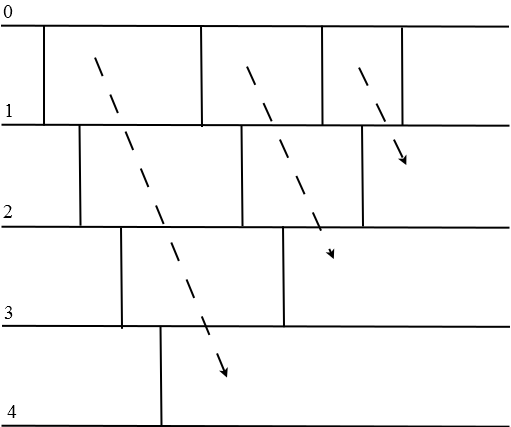
\includegraphics[scale=0.4]{img/4/sort_module.png}
		\caption{Sieć sortująca w układzie \textit{FPGA} -- źródło \cite{piszczek_15}}
		\label{fig:gmm_sort}
	\end{figure}	


\section{Zużycie zasobów}
\label{sec:fpga_zasoby}
\chapter{Ewaluacja zaimplementowanych algorytmów}
\label{cha:ewaluacja}

\section{Metodologia przeprowadzonych testów}
\label{sec:metodologia_testow}

Testy algorytmów opracowanych w Laboratorium Biocybernetyki AGH, zostały przeprowadzone zgodnie z metodologią opisaną w \cite{changedetection_15}. Sekwencje testowe pochodzą z bazy \textit{ChangeDetection} \cite{change_detection_web}. Tego typu podejście do ewaluacji zaimplementowanych algorytmów zostało wykorzystane między innymi w~\cite{kryjak_14_vibe, kryjak_14_pbas, janus_15}. Wszystkie metody zostały przetestowane z wykorzystaniem 31 sekwencji testowych podzielonych na 6 różnych kategorii. Zbiór testowy został tak dobrany, aby odwzorować jak największą liczbę sytuacji mogących wystąpić w rzeczywistym środowisku. Każda z kategorii została szczegółowo opisana w rozdziale \ref{sec:testy}.

Dla każdej sekwencji testowej zawartej w bazie, dostępny jest model wzorcowy tj. ręcznie anotowana maska obiektów (ang. \textit{ground truth}). Wzorzec zapisany jest jako obraz w skali szarości, gdzie piksele przyjmują jedną z pięciu wartości:

\begin{eqwhere}[2cm]
	\item[$0$] tło
	\item[$50$] cienie
	\item[$85$] obszar wyłączony z analizy
	\item [$175$] obszar trudny do zidentyfikowania (np. kontur otaczający ruchomy obiekt)
	\item [$255$] obiekt pierwszoplanowy \\
\end{eqwhere}  

\noindent Porównując ramki wyjściowe testowanego algorytmu z odpowiadającymi im ramkami modelu wzorcowego, można wyznaczyć następujące współczynniki:
\begin{eqwhere}[2cm]
	\item[$\small TP$] liczba pikseli poprawnie zakwalifikowanych jako pierwszy plan (ang. \textit{true positive})
	\item[$\small TN$] liczba pikseli poprawnie zakwalifikowanych jako tło (ang. \textit{true negative})
	\item[$\small FN$] liczba pikseli błędnie zakwalifikowanych jako tło (ang. \textit{false negative})
	\item[$\small FP$] liczba pikseli błędnie zakwalifikowanych jako pierwszy plan (ang. \textit{false positive})\\
\end{eqwhere}

\noindent Na podstawie wyznaczonych otrzymanych współczynników oblicza się 7 wskaźników jakości, określających dokładność metody:
%
\TabPositions{0.45\linewidth}
\begin{enumerate}[nolistsep]
	\item \textit{Recall (Re)} : \tab \small{$TP/(TP+FN)$}
	\item \textit{Specificity (Spec)} : \tab \small{$TN/(TN+FP)$}
	\item \textit{False Positive Rate (FPR)} : \tab \small{$FP/(FP + TN)$}
	\item \textit{False Negative Rate (FNR)} : \tab \small{$FN/(FN + TP)$}
	\item \textit{Percentage of Wrong Classifications (PWC)} : \tab \small{$100(FN + FP)/(TP + FN + FP + TN)$}
	\item \textit{Precision (Pr)} : \tab \small{$TP/(TP + FP)$}
	\item \textit{F-measure (F1)} : \tab \small{$2\frac{P_r*R_e}{P_r+R_r}$}\\
\end{enumerate}

Parametr \textit{Re} definiuje jaki procent pikseli pierwszoplanowych został rozpoznany. Analogiczną wartość dla pikseli reprezentujących tło określa parametr \textit{Se}. Parametry \textit{FPR} i \textit{FNR} są przeciwieństwem wartości opisanych wyżej i wynoszą odpowiednio $1-Se$ i $1-Re$. \textit{PWC} określa procent źle sklasyfikowany pikseli, natomiast \textit{Pr} informuje jaki procent spośród pikseli sklasyfikowanych jako pierwszoplanowe został rozpoznany prawidłowo.

\section{Szczegółowe test}
\label{sec:testy}
\chapter{Dalsze kierunki rozwoju}
\label{cha:kierunki_rozwoju}

\section{Poprawa algorytmów}
\label{sec:poprawa_algorytmow}

Oprócz standardowych wersji algorytmów, udało się także zaimplementować ich rozszerzone wersję, zdecydowanie poprawiając efektywność w specyficznych warunkach. W przypadku algorytmu \textit{ViBE} zaimplementowano moduł, który w znacznym stopniu eliminuje efekt drgającej kamery. Metoda \textit{PBAS} została natomiast rozszerzona o funkcjonalność detekcji obiektów statycznych. Kolejnym krokiem w~rozwoju algorytmów i zwiększania ich efektywności mogłoby być zaimplementowanie metody zawierającej oba te udoskonalenia. Dobrym punktem wyjścia może być w tym przypadku algorytm \textit{PBAS}, zawierający już moduł detekcji obiektów statycznych. Dodanie do takiej implementacji modułu wyliczającego przepływ optyczny powinno zostać wykonane bez dużych komplikacji. 

W Laboratorium Biocybernetyki AGH, w ramach pracy inżynierskiej \cite{janus_15} został częściowo zaimplementowany algorytm \textit{FTSG}. Jest to pierwsza implementacja tej metody w układzie reprogramowalnym. Nie udało się niestety opracować pełnej wersji, zaproponowanej przez autorów oryginalnej publikacji \cite{wang_14}. Zabrakło między innymi mechanizmu detekcji obiektów statycznych, który według założeń miał być bardzo podobny do tego wykorzystanego w metodzie \textit{PBAS}. Celem przyszłych badań może być próba wykorzystania opracowanego dla algorytmu \textit{PBAS} moduł analizy obiektów \textit{CCA} i zintegrowania go z algorytmem \textit{FTSG}. W celu poprawny dokładności można spróbować także zaimplementować mechanizm indeksacji obiektów w wariancie dwuprzebiegowym.

\section{Wzrost wydajności}
\label{sec:wzrost_wydajnosci}

Algorytmy przedstawione w niniejszej pracy starano się uruchomić w zarówno niskich (\textit{720x576}) jak i wysokich (\textit{1280x720}, \textit{1920x1080}) rozdzielczościach. Zamierzony cel udało się osiągnąć w przypadku podstawowych wersji algorytmu, niezawierających dodatkowych modułów odpowiedzialnych między innymi za redukcję drgań kamery lub detekcję obszarów statycznych. W wielu przypadkach wiązało się to niestety z obniżeniem dokładności algorytmu, na przykład z powodu redukcji modelu tła, bądź konieczności przejścia z przestrzeni kolorów \textit{RGB} do skali szarości. 

W przypadku rozszerzonych odmian algorytmów \textit{ViBE} oraz \textit{PBAS}, udało się jedynie zapewnić przetwarzanie w najniższej rozdzielczości. Istotną kwestią jest zatem optymalizacja przygotowanych implementacji sprzętowych. Wraz z postępem technologicznym i pojawianiem się nowych, wydajniejszych układów \textit{FPGA}, należy dążyć do obsługi wyższych rozdzielczości. Docelowo system wizyjny powinien przetwarzać obraz w rozdzielczości \textit{1920x1080} w 50 klatkach na sekundę, w dalszej przyszłości wymaganym standardem może stać się rozdzielczość \textit{4K (3840x2160 pikseli)}.

Wzrost wydajności systemów wizyjnych jest ograniczony przez kilka czynników. Jak zostało już podkreślone jedną z blokad jest aktualnie dostępny sprzęt. W niektórych przypadkach ujawnia się ograniczona ilość zasobów logicznych w układzie \textit{FPGA} lub dostępna pamięci \textit{RAM}. Jednak, aby zapewnić wzrost wydajności nie należy jedynie oczekiwać na postęp technologiczny. Każdy algorytm można w~pewnym stopniu zoptymalizować, poprzez uproszczenie logiki i zredukowanie ilości operacji wykonywanych w jednym cyklu. Taki zabieg może co prawda zwiększyć sumaryczną latencje, ale jednocześnie zapewni wyższą maksymalną częstotliwość pracy zegara. 


\section{Implementacja nowych rozwiązań}
\label{sec:implementacja_nowych_rozwiazan}

Mimo stosunkowo zadowalających efektów końcowych przygotowanych implementacji, nadal istnieje wiele kierunków w których algorytmy powinny być rozwijane. W przyszłości należy zastanowić się nad przygotowaniem między innymi dodatkowego mechanizmu detekcji dynamicznego tła i eliminacji jego wpływu na pracę algorytmu. Kolejnym wartym uwagi zagadnieniem jest prawidłowa detekcja cieni i ich odróżnienie od rzeczywistych obiektów. Oba zagadnienia są tematami bardzo rozległymi, które nie zostały do tej pory poruszone w ramach badań w Laboratorium Biocybernetyki AGH.

Kolejną drogą rozwoju może być próba tworzenia implementacji sprzętowych istniejących już algorytmów. Autorzy publikacji na różnego rodzaju konferencjach poświęconych systemom wizyjnym prezentują nowatorskie rozwiązania, często jednak nowy algorytm przedstawiany jest jedynie od strony teoretycznej. Mimo, że model programowy przygotowany na komputerze klasy PC daje świetne rezultaty w testach, jego zastosowanie w rzeczywistym systemie wizyjnym jest niemożliwe dopóki nie powstanie dedykowana implementacja sprzętowa. Przykładem takiego działania może być algorytm \textit{Flux Tensor}, którego pierwsza implementacja sprzętowa \cite{janus_16_flux} została przygotowana właśnie w Laboratorium Biocybernetyki AGH.
\chapter{Zakończenie}
\label{cha:zakonczenie}


% itd.
% \appendix
% \include{dodatekA}
% \include{dodatekB}
% itd.

\printbibliography

\end{document}
